\documentclass[11pt, oneside]{report}

\usepackage{geometry}
\geometry{a4paper}
\usepackage{amsmath}
% \setmonofont[Scale=0.85]{Menlo}
\usepackage{enumitem}
\usepackage{amssymb}
\usepackage{hyperref}
\usepackage{pgfplots}
\hypersetup{linktoc=all}
\usepackage[T1]{fontenc}
\usepackage{newpxmath}
\usepackage{color}
\usepackage{mathspec}
\setmainfont [Ligatures={Common,TeX}]{Palatino Linotype} 
\usepackage{setspace}
\usepackage{wrapfig}
\usepackage{tikz}
\usepackage{subcaption}


\newcommand{\comment}[1]{}
\newcommand{\pcomment}[1]{}
\DeclareMathOperator*{\argmin}{argmin}
\newfontfamily\legends{Arial}

\linespread{1.2}

%\renewcommand{\abstractname}{Abstract}



\title{Automated Bee Pose Estimation}
\author{Jakub Nabaglo, u5558578}
\date{Semester 2, 2015}

\begin{document}
\maketitle

\begin{abstract}
    Bees are crucial to our food supply and economy. Bee researchers possess inadequate data regarding bee populations. A crowdsourced approach to collecting such data may be feasible, but is hindered by the lack of trained bee taxonomists. An automated tool being able to classify bee species from images may be valuable. This project presents an approach to automated bee pose estimation that the author believes to be the first step towards automated bee classification from images.
\end{abstract}

\tableofcontents\newpage

\chapter{Motivation}
    Bees play a crucial role in the environment. Acting as important pollinators for numerous flowering crops, they are relied upon by our food supply and our economy, being responsible for an estimated \$200\,billion per annum in crop production (Agriculture and Consumer Protection Department of the Food and Agriculture Organization of the United Nations, 2005). Further, bees form an integral part of our ecosystems.

    Bee populations worldwide have been decreasing for decades. Research into the causes of this decline, and ways of limiting it, is crucial. It is challenged by the difficulty in tracking bee populations. That difficulty is due to a number of factors, including a lack of trained taxonomists as well as limited resources being devoted to recording bee specimens.

    A software tool capable of automatically classifying bee species from images would hence be valuable, allowing scientists and amateurs to document bee sightings by species and thus increasing the amount of data available for research. An extension of this would be a crowdsourcing application that would enable non-professionals to photograph bees that they encounter, storing the specimen species along with a geotag and a timestamp in a public database.

\chapter{Related works}
    Santana et al. (2014) have performed automated bee classification based on bee wing images labelled with the bee species and annotated with landmarks. Their process extracts wing features such as `vein length, width, curvature, angles and the area of all cells' (Santana et al, 2014, p. 253) that may be input into a generic classifier.

    \begin{wrapfigure}{l}{0.5\textwidth}
        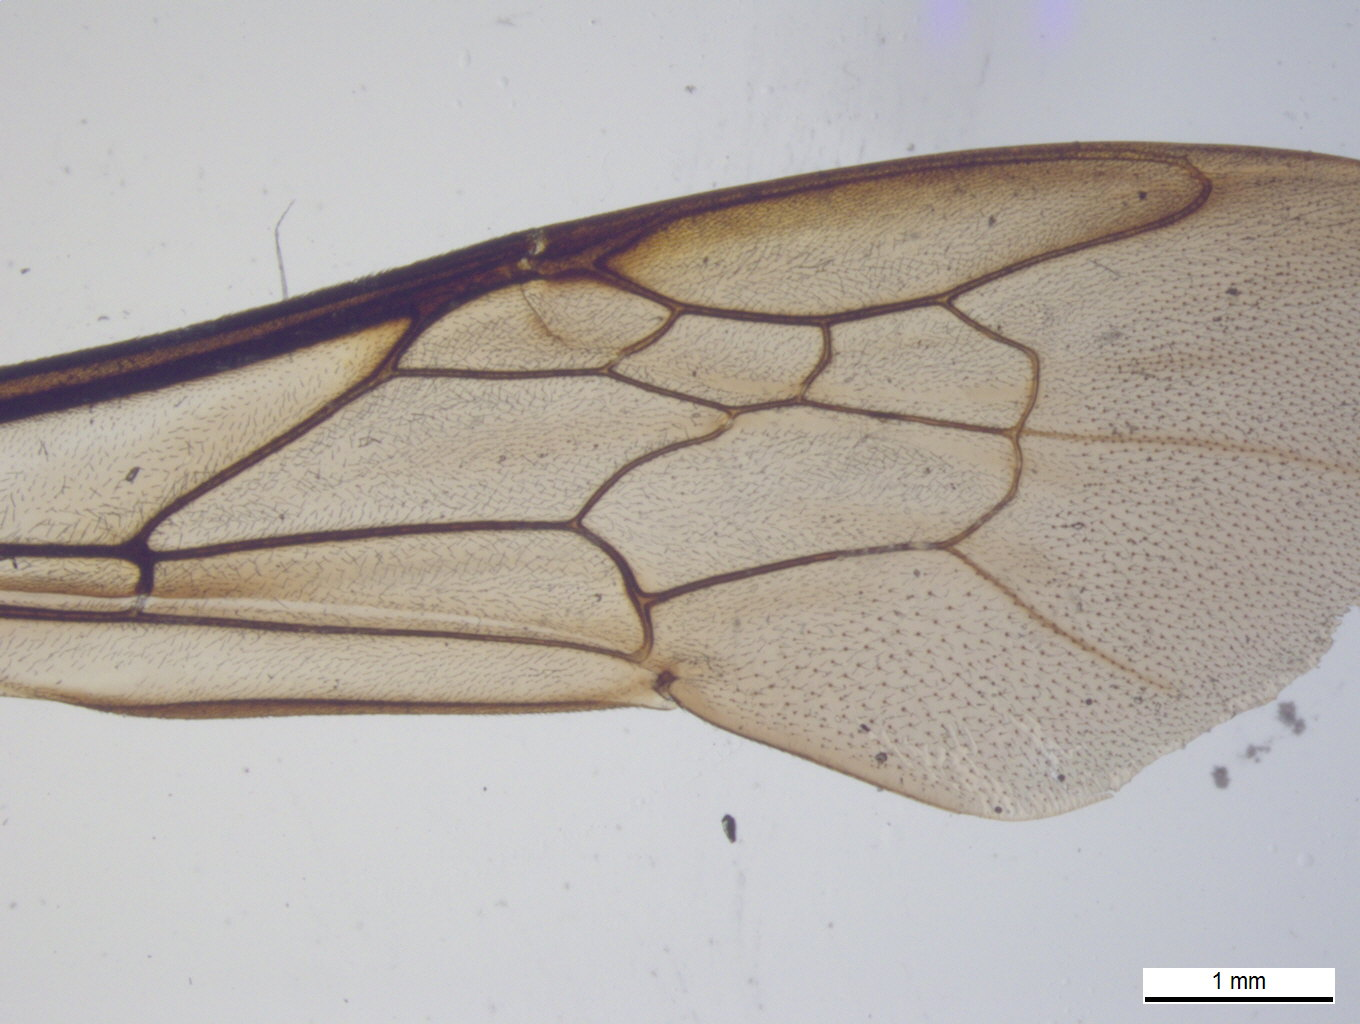
\includegraphics[width=0.5\textwidth]{santana.jpg}
        \caption{Image typical of the dataset used by Santana et al. (2014)}
        \label{fig:santana_example}
    \end{wrapfigure}

    Their approach presents several problems. In order to reliably extract features, the training and testing photographs must be captured in a highly uniform manner: the wing images must be of a high resolution and have a plain white background. An example image is shown in figure \ref{fig:santana_example}. If the goal is to enable amateurs to photograph bees and automatically classify them, the user cannot be expected to possess the equipment or motivation necessary for such consistent specimen collection.

    Further, in the work of Santana et al. (2014), images used for training and prediction must be annotated with landmarks before relevant features can be extracted. This, again, is not something an an amateur user should be expected to do.

    As such, it is necessary to develop a method to classify bees regardless of their position or orientation in the image, without requiring the user to take the photograph in a particular way, and not necessitating that they annotate landmarks. It is a logical first step to train a machine to detect the pose of the bee, as well as the bee parts useful for classification.

    Yang and Ramanan (2011) describe a model for human pose estimation. It is a supervised learning model that trains on photographs of humans that are annotated with positions of their body parts. In addition, a tree model must be defined on these parts. The tree is used in a graphical model to take advantage of relationships between body parts during training and detection.

    Although their work describes human pose estimation, it may conceivably be applied to bee pose estimation. Challenges may include the small size of some bee parts, such as antennae or legs, as well as the tendency for bee images to occlude parts: these may lower the accuracy of part detections. Large variations in bee poses may also be problematic, as this reduces the utility of the graphical model.

\chapter{Method}
    Experiments to perform bee pose estimation were conducted on the BEES dataset. From the BEES dataset, 250 images with all seven parts labelled were selected and split into six sets of 50. Of these, four were used for training and two were used for testing. The images in BEES deemed unsuitable for use in experiments due to bee part occlusions were used as a basis for a negative training set: bees were cropped out of these images, leaving only the background.

    The algorithm described by Yang and Ramanan (2011) was used as a basis for the experiments. A tree structure was defined on the seven bee parts labelled in BEES, with the head as the root; the antennae and the thorax as children of the head; and the wings and the abdomen as children of the thorax.

    Following training on the four training sets, predictions were made on the testing set. The testing set predictions were then displayed and visually inspected for correctness and accuracy.

    Experiments were run to determine the optimal model parameters: the optimal size of HOG cells, the optimal number of parts to use in the graphical model, and the optimal amount of data augmentation.

\section{Algorithm}
    The algorithm used is based on the work of Yang and Ramanan (2011). It is described in more detail in their paper. A summary is provided here.

    Let $I$ be an image.

    Let $K \in\mathbb{N}$ be the number of bee parts considered, such as the head, or the wings. Then let $i \in \{1,\dots,K\}$ denote a bee part, such as the head or the left wing.

    Let $T\in\mathbb{N}$ be the number of components in the mixtures model of each part.  Let $t_i \in\{1,\dots,T\}$ be the `type' of part $i$. As an example, a bee wing can be of the folded type or of the extended type. Let $\vec{t}=(t_1,\dots,t_K)^\intercal$.

    Let $p_i=(x_i,y_i)$ be the position of part $i$ in the image $I$. Let $\vec p=(p_1,\dots,p_K)$.

    We wish to assign scores to configurations of parts. For all parts $i, j \in \{1,\dots,K\}$, let $b_i^{t_i}$ be a parameter that is greater for assignments of particular types $t_i$ to $i$. In addition, let $b_{i,j}^{t_i,t_j}$ be greater for particular co-assignments of types $t_i$ and $t_j$ to $i$ and $j$ respectively: for example, one wing being extended may make it more likely that the other wing is also extended. Define the function   \[
        S(\vec t) = \sum_{i\in V}b_i^{t_i}+\sum_{(i,j)\in E}b_{i,j}^{t_i,t_j}\textrm{,}
    \]
    where $(V,E)$ is a $K$-node relational graph, where the nodes correspond to parts and edges correspond to relation constraints between part types.

    It is now possible to define the full score for a configuration of part types $\vec t$ and part positions $\vec p$ in an image $I$: \[
        S(I,\vec p, \vec t) = S(\vec t) + \sum_{i\in V}w^{t_i}_i\cdot\phi(I,p_i)
        + \sum_{(i,j) \in E}w_{i,j}^{t_i,t_j}\cdot\psi(p_i-p_j)\textrm{,}
    \]
    where $w_i^{t_i}$ and $w_{i,j}^{t_i,t_k}$ are learned parameters; where $\phi(I, p_i)$ is a HOG descriptor extracted from $p_i$ in $I$; and where $\psi(p_i-p_j)=\left((x_i-x_j)\;(x_i-x_j)^2\;(y_i-y_j)\;(y_i-y_j)^2\right)^\intercal$.

    Observing that $S(I,\vec p, \vec t)$ is linear in parameters $b_i^{t_i}$, $b_{i,j}^{t_i,t_j}$, $w_i^{t_i}$ and $w_{i,h}^{t_i,t_j}$, we can define $\vec\beta = \left(w_i^{t_i}, \dots, w_{i,h}^{t_i,t_j}, \dots, b_i^{t_i}, \dots, b_{i,j}^{t_i,t_j}, \dots\right)^\intercal$ such that $S\left(I, \vec p, \vec t\right)=\vec\beta\cdot\Phi\left(I, \vec p, \vec t\right)$ for some function $\Phi$. Learning then solves the optimisation problem: \begin{align*}
        \argmin_{w_i^{t_i}, \dots, w_{i,h}^{t_i,t_j}, \dots, \xi_i, \ldots \geq 0} &\quad\frac12\beta\cdot\beta+C\sum_n\xi_n\\
        \textrm{s.t.}\quad\forall n \in \textrm{pos} & \quad\beta\cdot\Phi(I_n, p_n, t_n) \geq 1-\xi_n \\
        \forall n \in \textrm{pos} \;\forall (p_i, t_i) & \quad\beta\cdot\Phi(I_n, p_i, t_i) \leq 1-\xi_n\textrm{.}
    \end{align*}
    The above enforces that positive examples should have scores that are greater than 1, while negative examples should score less than $-1$ for all possible part positions and types. $\xi_n$ are slack variables that penalise violations of these constraints. $C>0$ is a constant.

    Inference is then equivalent to maximising $S(I,\vec p, \vec t)$ over $\vec p$ and $\vec t$. This can be done efficiently with dynamic programming.

\section{Models for bees}
    \begin{figure}[t]
        \centering
        \begin{minipage}{0.4\textwidth}
            \centering
            \begin{tikzpicture}[scale=2.5]
                \tikzstyle{vertex}=[circle, draw=black, fill=white, line width=0.5mm, minimum size=25pt, inner sep=0pt]
                \tikzstyle{edge} = [draw, line width=1mm, -]

                \node[vertex,label=above:{Head}] (a) at (0,2) {};
                \node[vertex,label=right:{Thorax}] (b) at (0,1) {};
                \node[vertex,label=below:{Abdomen}] (c) at (0,0) {};

                \foreach \source/ \dest in {a/b, b/c}
                \path[edge] (\source) -- (\dest);
            \end{tikzpicture}
            \caption{The three-part model}
            \label{fig:3part_graph}
        \end{minipage}\hfill
        \begin{minipage}{0.55\textwidth}
            \centering
            \begin{tikzpicture}[scale=2.5]
                \tikzstyle{vertex}=[circle, draw=black, fill=white, line width=0.5mm, minimum size=25pt, inner sep=0pt]
                \tikzstyle{edge} = [draw, line width=1mm, -]

                \node[vertex,label=above:{Head}] (a) at (1,2) {};
                \node[vertex,label=right:{Thorax}] (b) at (1,1) {};
                \node[vertex,label=below:{Abdomen}] (c) at (1,0) {};
                \node[vertex,label=below:{Left wing}] (d) at (0,0) {};
                \node[vertex,label=below:{Right wing}] (e) at (2,0) {};
                \node[vertex,label=above:{Left antenna}] (f) at (0,2) {};
                \node[vertex,label=above:{Right antenna}] (h) at (2,2) {};

                \foreach \source/ \dest in {a/b, b/c, b/d, b/e, a/f, a/h}
                \path[edge] (\source) -- (\dest);
            \end{tikzpicture}
            \caption{The seven-part model}
            \label{fig:7part_graph}
        \end{minipage}
    \end{figure}
    \subsection{Three-part model}
        One of the bee part models considered is a three-part model consisting of the head, the thorax, and the abdomen, with edges running from the head to the thorax and from the thorax to the abdomen. This is illustrated in figure \ref{fig:3part_graph}.

        Since it uses only three, prominent bee parts, there are few images in the BEES dataset in which one of the parts is occluded. As such, there is a larger dataset available for training and testing.

    \subsection{Seven-part model}
        Another model considered is a seven-part model consisting of the head, the thorax, the abdomen, the left antenna, the right antenna, the left wing, and the right wing. There are edges running from the head to the thorax, from the thorax to the abdomen, as well as from the head to the antennae, and from the thorax to the wings. It is illustrated in figure \ref{fig:7part_graph}.

        Due to the higher number of parts used, it is more likely that in a particular image, a necessary part is occluded or missing. Hence, if the seven-part model is used, then the number of images available for training and testing is reduced. However, it is possible that the additional data points have a positive impact significant enough to compensate for a reduced training set.

\section{Evaluation}
    In our experiments, two measures were used to quantify the quality of predictions: the Probability of Correct Keypoint (PCK) and the Average Precision of Keypoints (APK). They are sourced from Yang Y. and Ramanan D. (2013).

    \subsection{Probability of Correct Keypoint}
        For each image, each inferred part location is deemed either correct or incorrect. A part location is correct if it is within a threshold $\alpha\gamma$ of the ground-truth location, where $\alpha>0$ is a constant and $\gamma$ is a scaling factor equal to the distance between two particular parts in the image, in our case the head and the thorax. The percentage of correct keypoints is then computed for each part.

    \subsection{Average Precision of Keypoints}
        Part joints can be thought of as objects to be detected. Hence, a precision-recall curve (Everingham M. et al., 2010) can be used to evaluate this object detection accuracy. Due to this, APK penalises both false-negatives as well as false-positives.

\chapter{Results}
    We show the results of our experiments with varying HOG cell sizes, varying numbers of parts in our model and varying amounts of data augmentstion.
    \section{HOG cell size}
        We compared the accuracy and correctness of HOG cell sizes of $3\times3$, $4\times4$, $5\times5$, $6\times6$, $8\times8$, $10\times10$, $12\times12$, and $16\times16$ pixels. The correctness is shown in figure \ref{fig:hog_pck} and the accuracy is plotted in figure \ref{fig:hog_apk}.

        It can be clearly seen that HOG cells of size $4\times4$ perform best. This is not an effect of noise: a clear trend is visible, where both the correectness and accuracy peak at the HOG size of $4\times4$.

        These statistics may be verified visually. Sample predictions are shown in figures \ref{fig:hog_vis1}, \ref{fig:hog_vis2}, and \ref{fig:hog_vis3}.

        The low optimal resolution of the HOG cells may be justified by the low resolutions of the bees: they form small areas of images that are themselves of low resolution.

        \begin{figure}
            \centering
            \begin{minipage}{0.48\textwidth}
                \centering
                    \begin{tikzpicture}
                        \begin{axis}[width=\textwidth,
                            xlabel=Size of HOG cell,
                            ylabel=Probability of Correct Keypoint (\%)]
                        \addplot[only marks,color=red,mark=triangle*] coordinates {
                            ( 3, 60)
                            ( 4, 63)
                            ( 5, 59)
                            ( 6, 43)
                            ( 8, 40)
                            ( 10, 6)
                            ( 12, 5)
                            ( 16, 14)
                        };
                        \addplot[only marks,color=green,mark=*] coordinates {
                            ( 3, 60)
                            ( 4, 70)
                            ( 5, 65)
                            ( 6, 49)
                            ( 8, 47)
                            ( 10, 35)
                            ( 12, 28)
                            ( 16, 28)
                        };
                        \addplot[only marks,color=blue,mark=triangle*, mark options={rotate=180}] coordinates {
                            ( 3, 51)
                            ( 4, 50)
                            ( 5, 43)
                            ( 6, 35)
                            ( 8, 31)
                            ( 10, 15)
                            ( 12, 7)
                            ( 16, 12)
                        };
                        \addplot[only marks,color=black,mark=square*] coordinates {
                            ( 3, 57)
                            ( 4, 61)
                            ( 5, 55.7)
                            ( 6, 42.3)
                            ( 8, 39.3)
                            ( 10, 18.7)
                            ( 12, 13.3)
                            ( 16, 18)
                        };
                        \legend{Head, Thorax, Abdomen, Mean}
                        \end{axis}
                    \end{tikzpicture}
                \caption{PCK by HOG cell size for the three-part model}
                \label{fig:hog_pck}
            \end{minipage}\hfill
            \begin{minipage}{0.48\textwidth}
                \centering
                \begin{tikzpicture}
                    \begin{axis}[width=\textwidth,
                        xlabel=Size of HOG cell,
                        ylabel=Average Precision of Keypoints (\%)]
                    \addplot[only marks,color=red,mark=triangle*] coordinates {
                        ( 3, 45.2)
                        ( 4, 56.2)
                        ( 5, 51.2)
                        ( 6, 31.1)
                        ( 8, 30.4)
                        ( 10, 5.5)
                        ( 12, 7.3)
                        ( 16, 9.4)
                    };
                    \addplot[only marks,color=green,mark=*] coordinates {
                        ( 3, 50.3)
                        ( 4, 56.2)
                        ( 5, 53.3)
                        ( 6, 37.8)
                        ( 8, 41.1)
                        ( 10, 16.3)
                        ( 12, 10.6)
                        ( 16, 16.5)
                    };
                    \addplot[only marks,color=blue,mark=triangle*, mark options={rotate=180}] coordinates {
                        ( 3, 38.5)
                        ( 4, 46.5)
                        ( 5, 33.2)
                        ( 6, 25.2)
                        ( 8, 24)
                        ( 10, 6.6)
                        ( 12, 5.6)
                        ( 16, 8.7)
                    };
                    \addplot[only marks,color=black,mark=square*] coordinates {
                        ( 3, 44.7)
                        ( 4, 53)
                        ( 5, 45.9)
                        ( 6, 31.4)
                        ( 8, 31.8)
                        ( 10, 9.5)
                        ( 12, 7.9)
                        ( 16, 11.5)
                    };
                    \legend{Head, Thorax, Abdomen, Mean}
                    \end{axis}
                \end{tikzpicture}
                \caption{APK by HOG cell size for the three-part model}
                \label{fig:hog_apk}
            \end{minipage}
        \end{figure}

        \begin{figure}[p]
            \centering
            \begin{subfigure}[b]{0.3\textwidth}
                \centering
                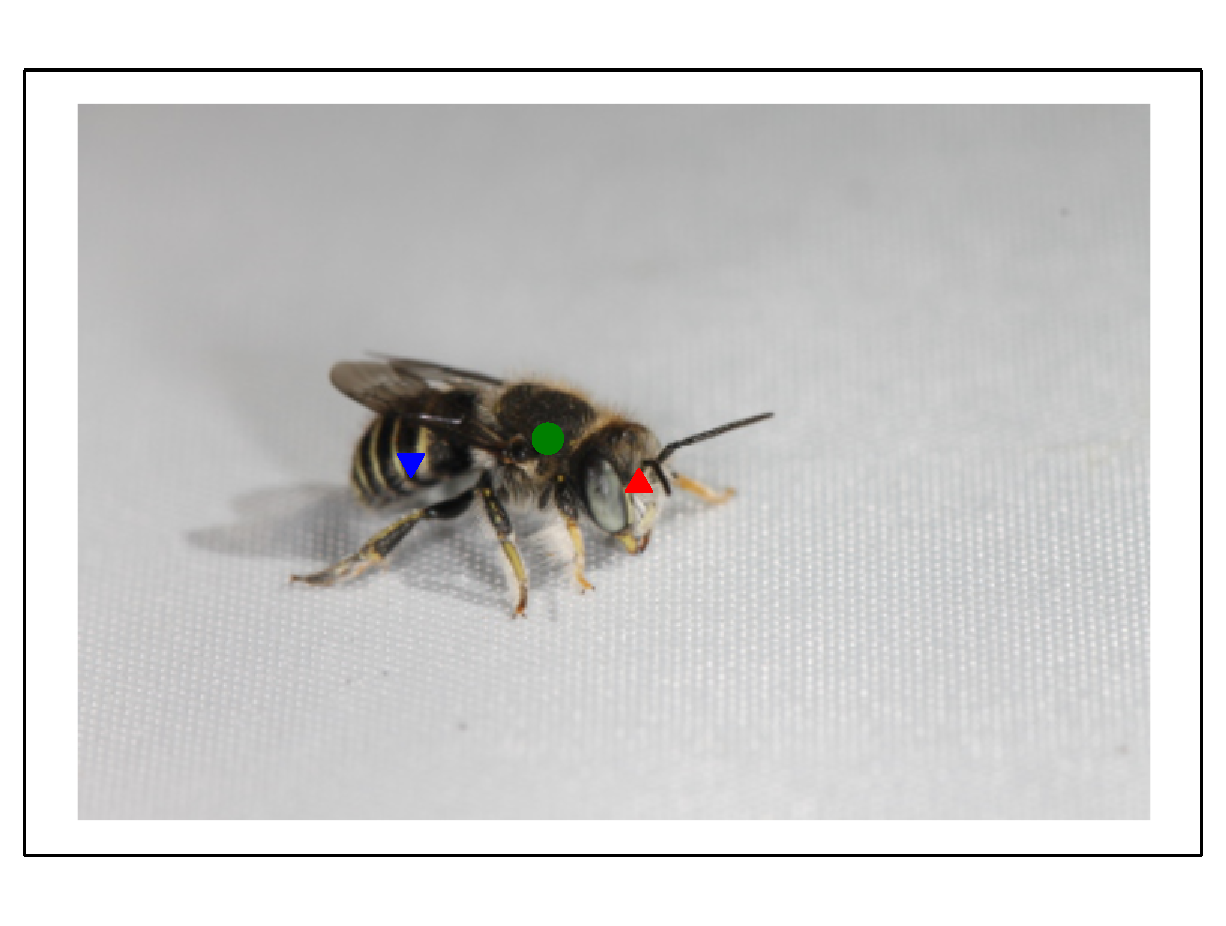
\includegraphics[width=\textwidth]{hog3_1.pdf}
                \caption{$3\times3$ HOG cells}
            \end{subfigure}
            \begin{subfigure}[b]{0.3\textwidth}
                \centering
                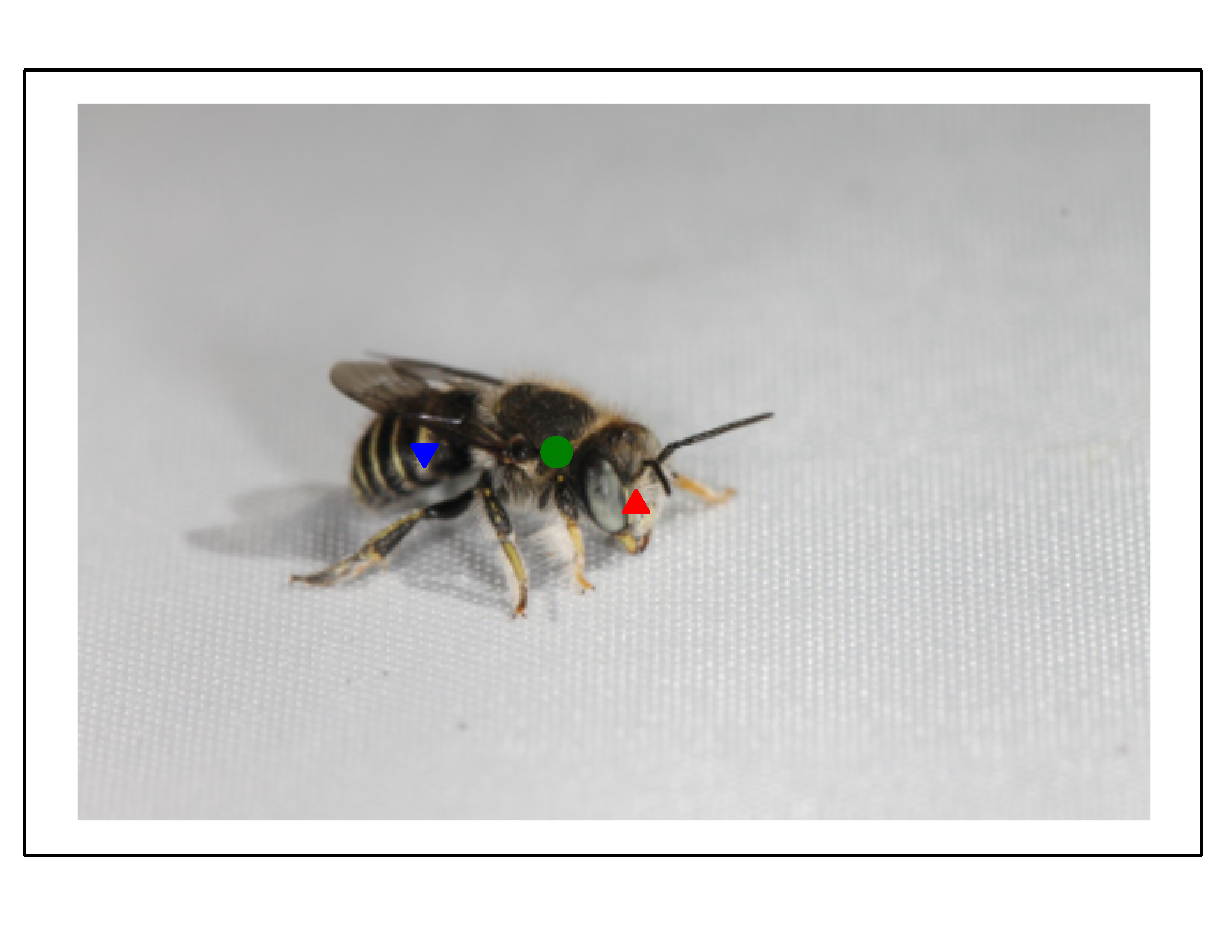
\includegraphics[width=\textwidth]{hog4_1.pdf}
                \caption{$4\times4$ HOG cells}
            \end{subfigure}
            \begin{subfigure}[b]{0.3\textwidth}
                \centering
                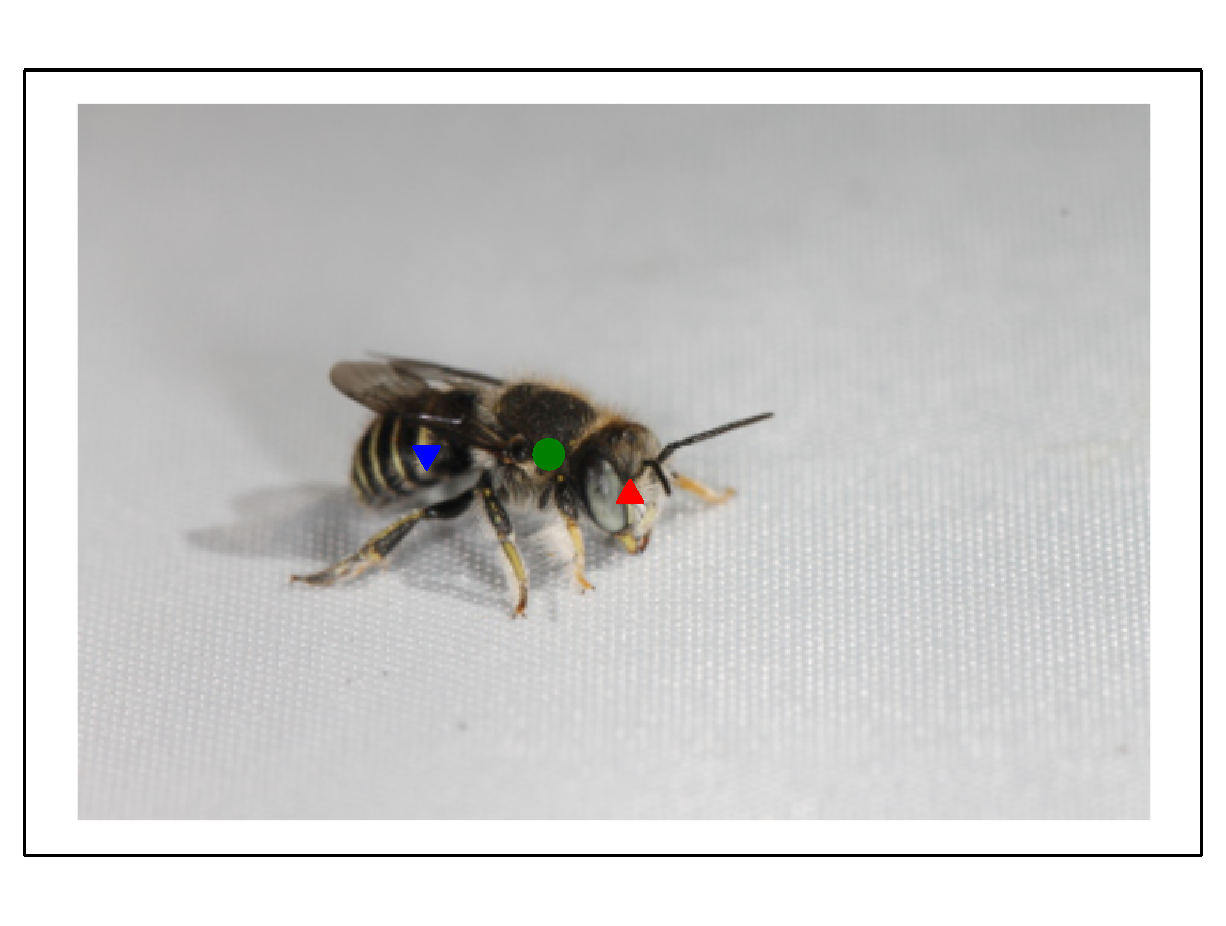
\includegraphics[width=\textwidth]{hog5_1.pdf}
                \caption{$5\times5$ HOG cells}
            \end{subfigure}
            \begin{subfigure}[b]{0.3\textwidth}
                \centering
                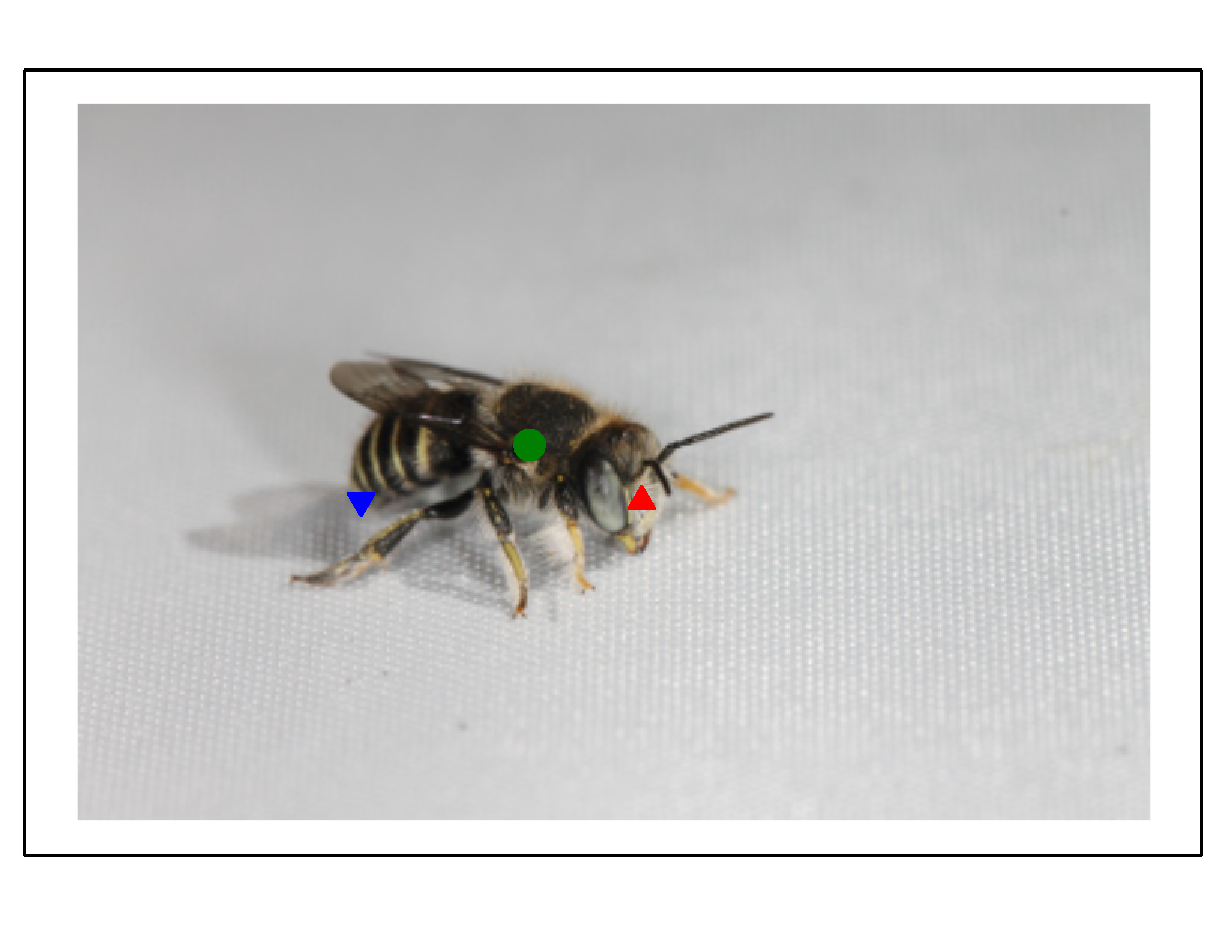
\includegraphics[width=\textwidth]{hog6_1.pdf}
                \caption{$6\times6$ HOG cells}
            \end{subfigure}
            \begin{subfigure}[b]{0.3\textwidth}
                \centering
                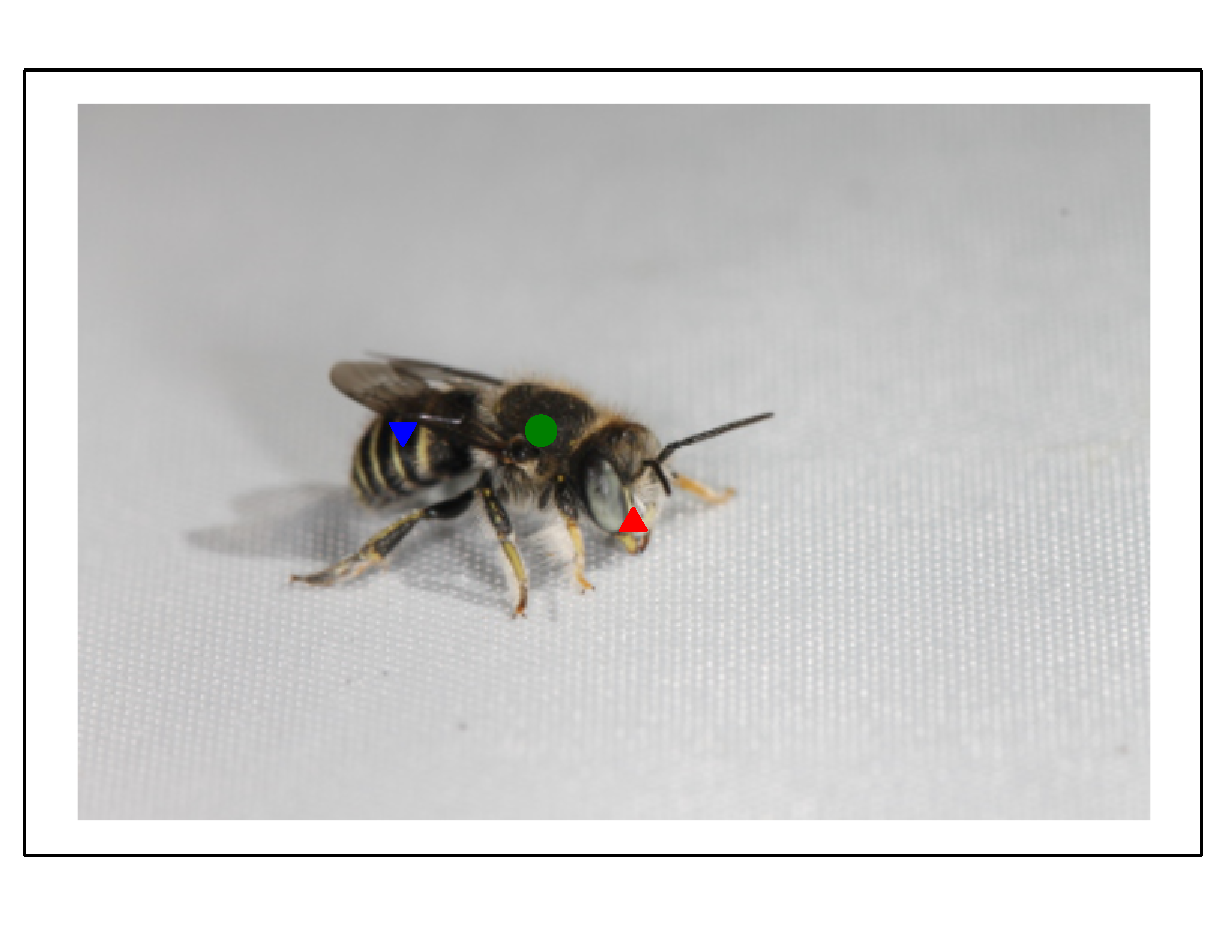
\includegraphics[width=\textwidth]{hog8_1.pdf}
                \caption{$8\times8$ HOG cells}
            \end{subfigure}
            \begin{subfigure}[b]{0.3\textwidth}
                \centering
                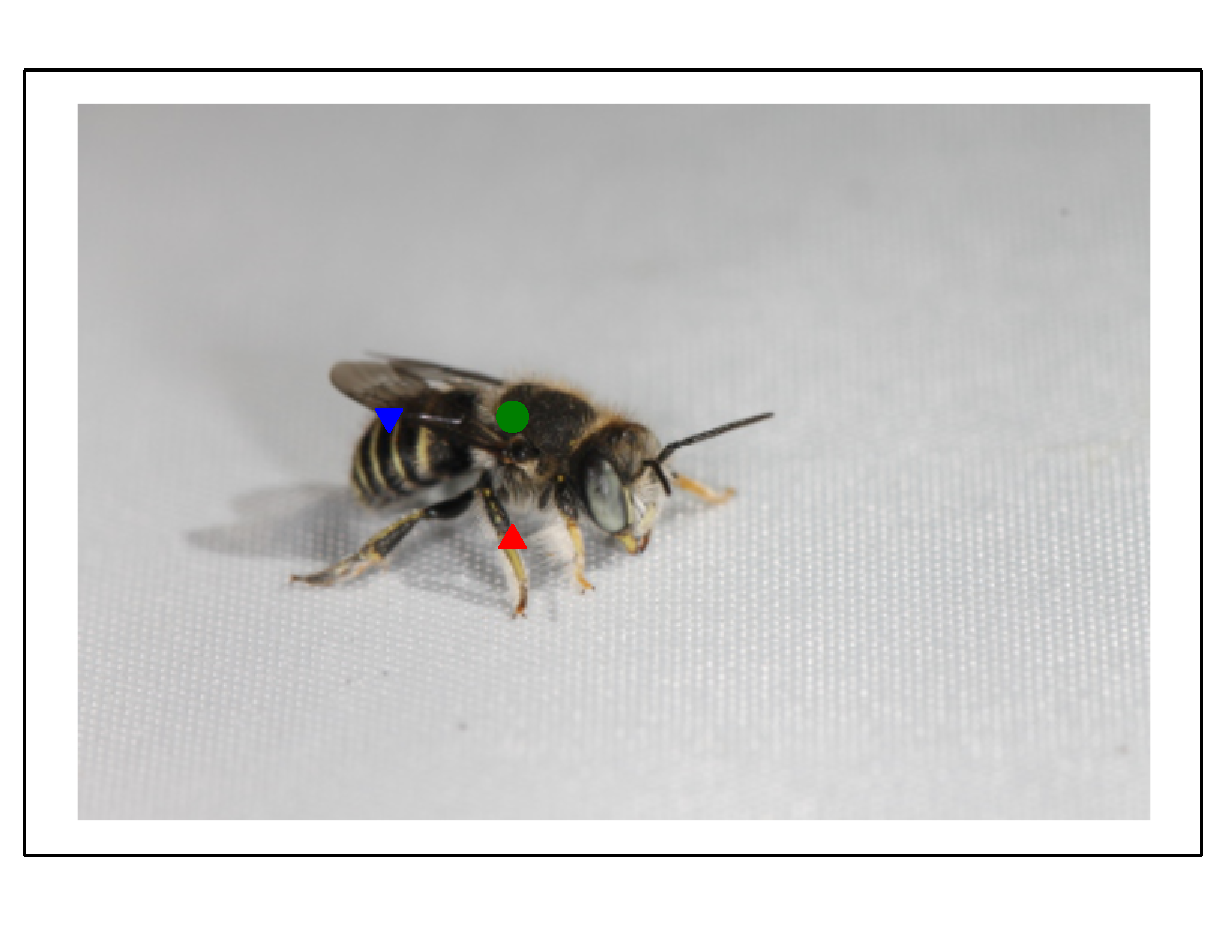
\includegraphics[width=\textwidth]{hog10_1.pdf}
                \caption{$10\times10$ HOG cells}
            \end{subfigure}
            \begin{subfigure}[b]{0.3\textwidth}
                \centering
                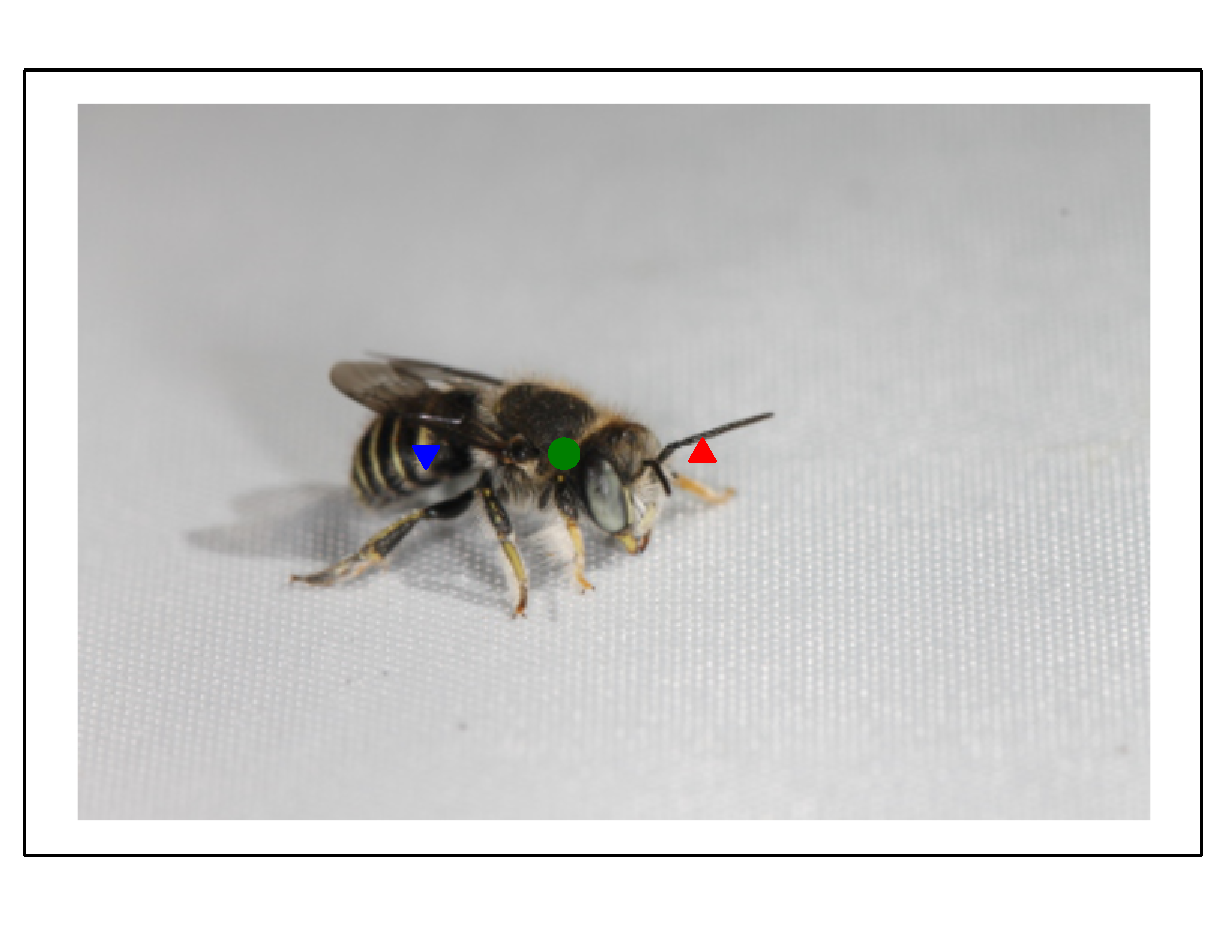
\includegraphics[width=\textwidth]{hog12_1.pdf}
                \caption{$12\times12$ HOG cells}
            \end{subfigure}
            \begin{subfigure}[b]{0.3\textwidth}
                \centering
                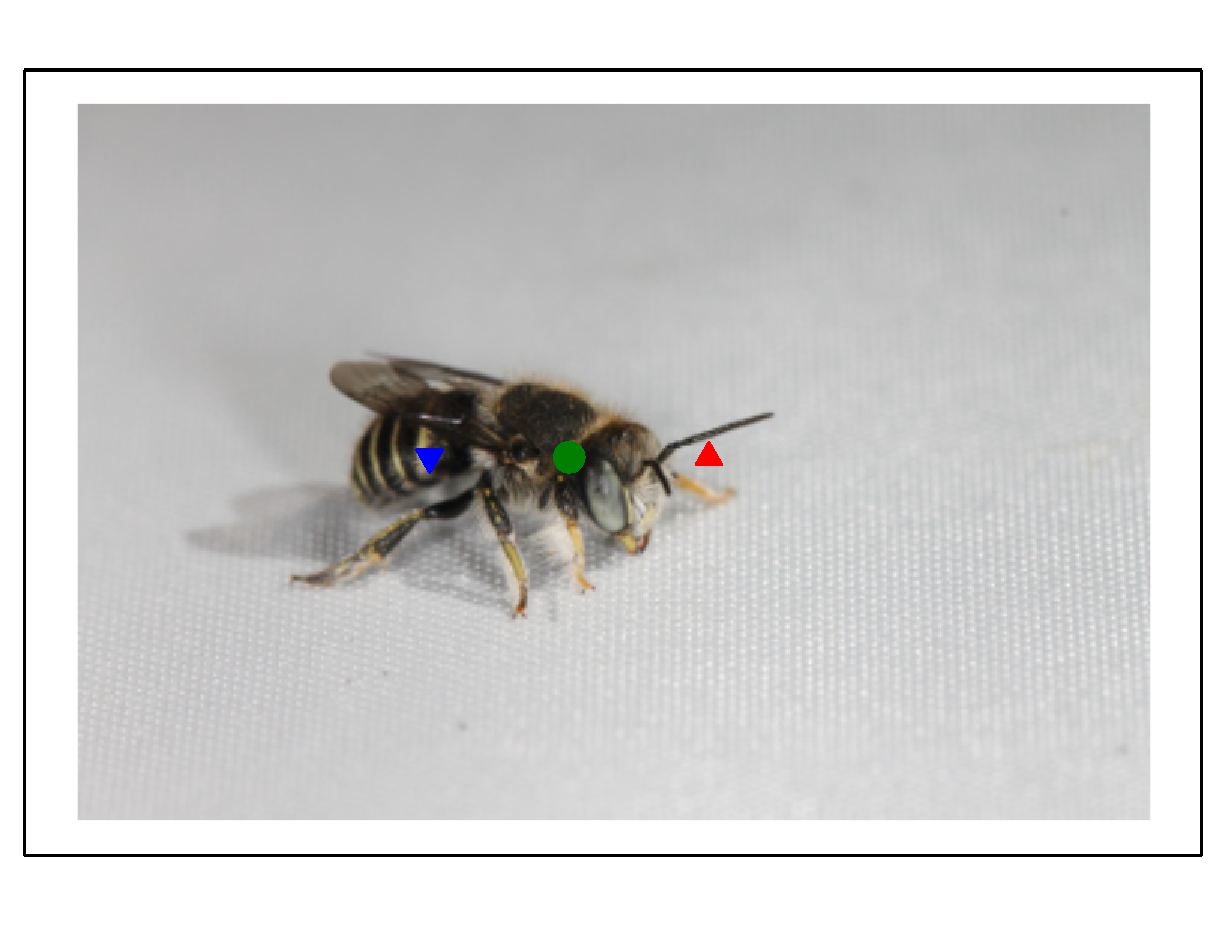
\includegraphics[width=\textwidth]{hog16_1.pdf}
                \caption{$16\times16$ HOG cells}
            \end{subfigure}
            \begin{subfigure}[b]{0.3\textwidth}
                \centering
                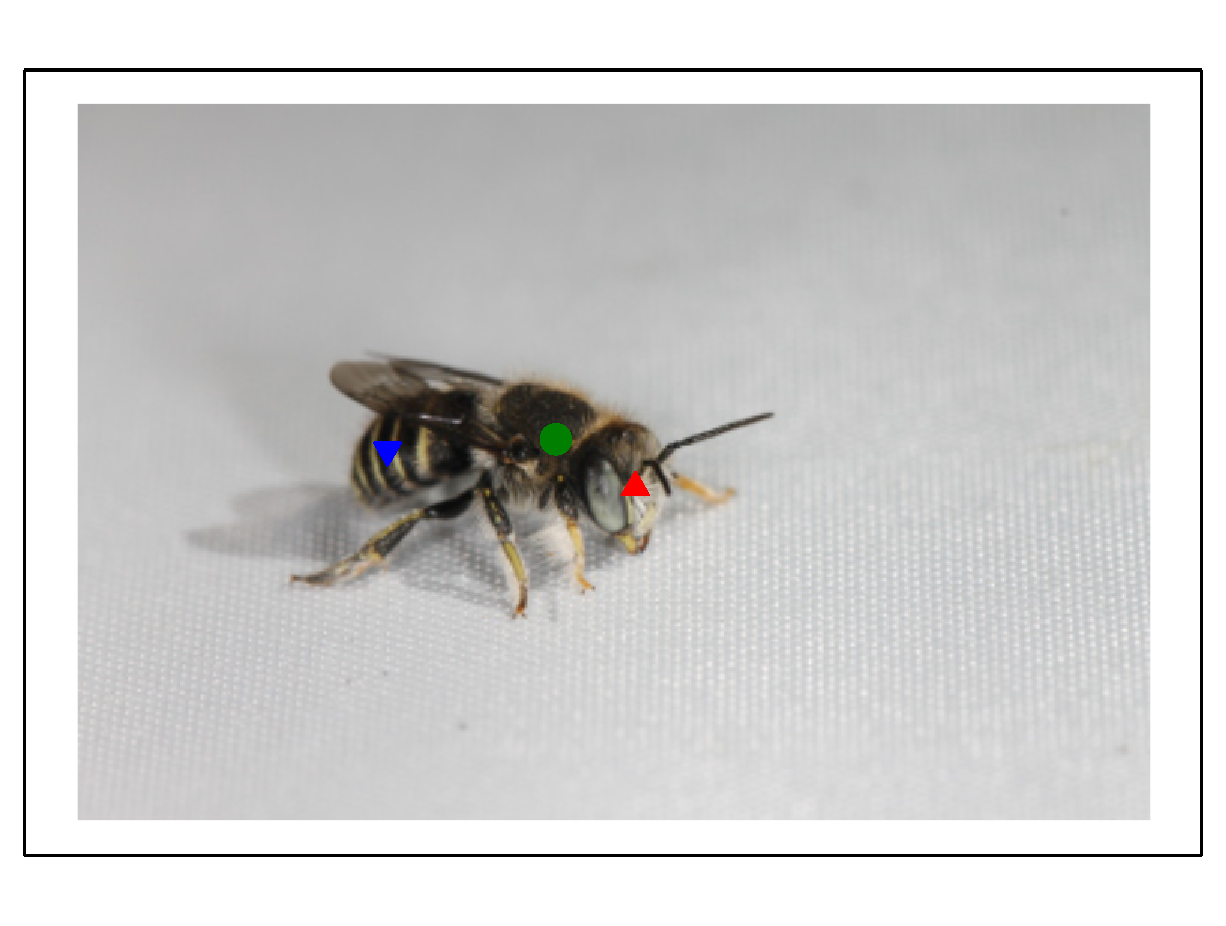
\includegraphics[width=\textwidth]{hog_gt1.pdf}
                \caption{Ground truth}
            \end{subfigure}

            \hspace{0pt}

            \begin{subfigure}[b]{0.2\textwidth}
                \centering
                \fbox{\begin{minipage}{\textwidth}
                    \begin{tabular}{c l}
                    {\legends\color{red}{\rotatebox[origin=c]{0}{▲}}}&Head\\
                    {\legends\color{green}{●}}&Thorax\\
                    {\legends\color{blue}{\rotatebox[origin=c]{180}{▲}}}&Abdomen
                    \end{tabular}
                \end{minipage}}
            \end{subfigure}
            \caption{Three-part model predictions on sample test image by HOG cell size}
            \label{fig:hog_vis1}
        \end{figure}

        \begin{figure}[p]
            \centering
            \begin{subfigure}[b]{0.3\textwidth}
                \centering
                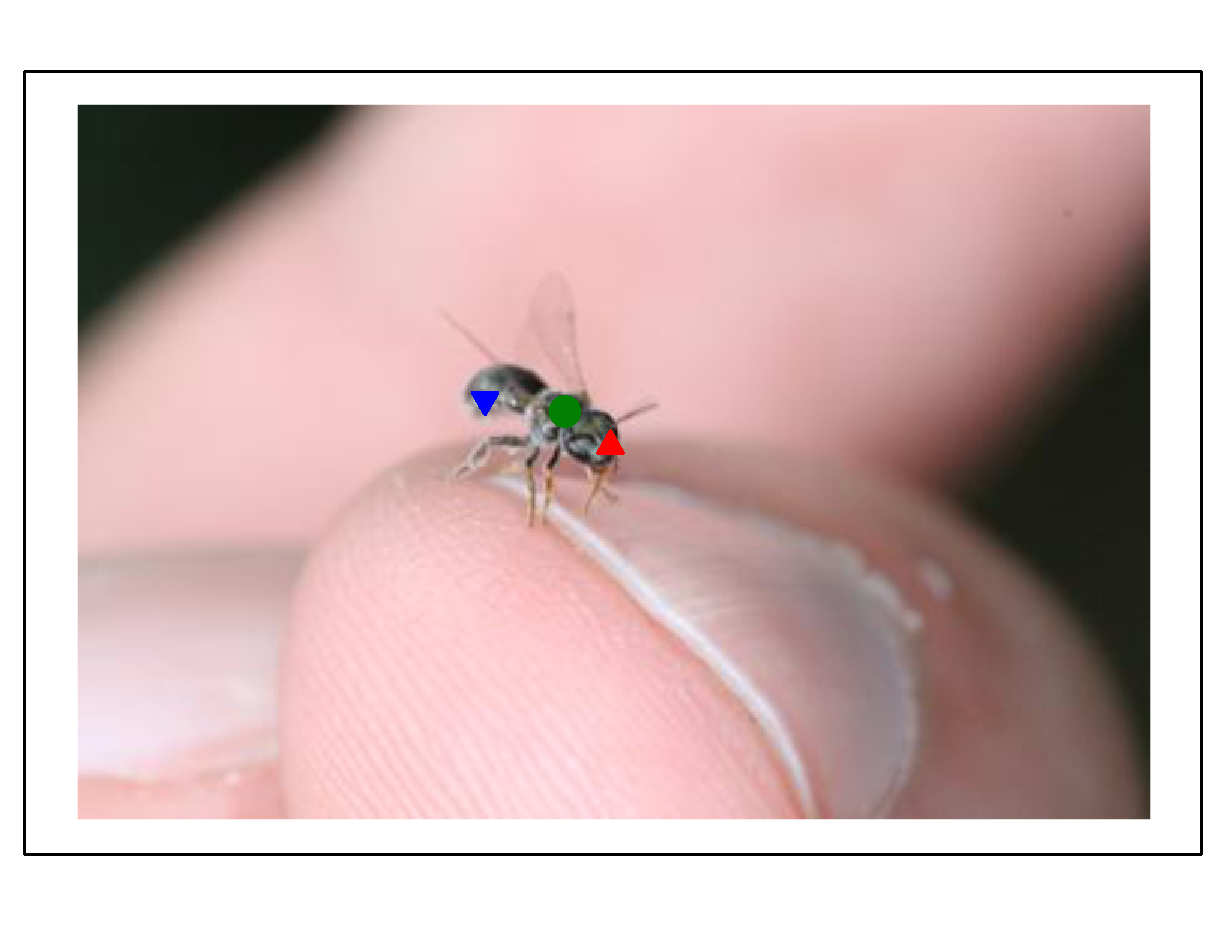
\includegraphics[width=\textwidth]{hog3_2.pdf}
                \caption{$3\times3$ HOG cells}
            \end{subfigure}
            \begin{subfigure}[b]{0.3\textwidth}
                \centering
                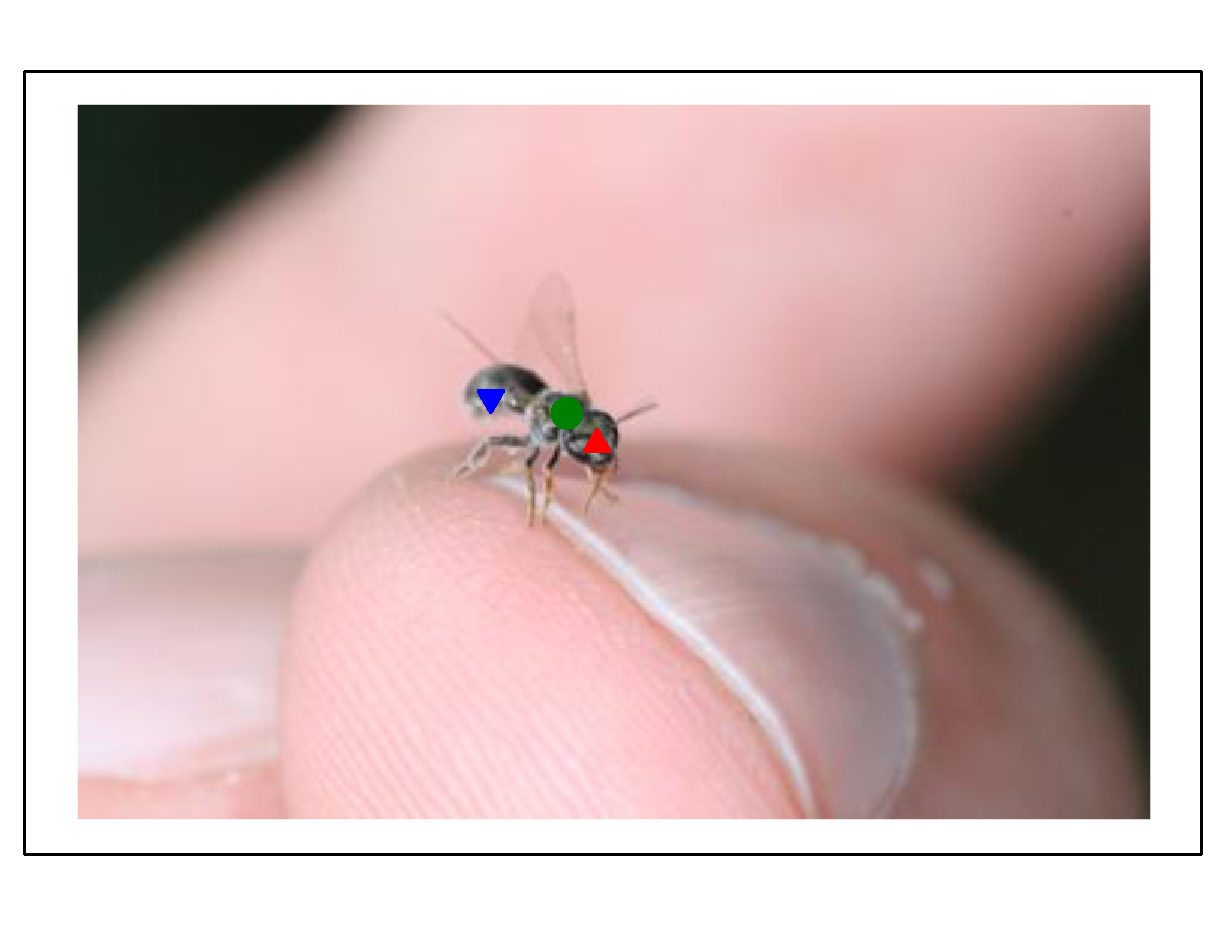
\includegraphics[width=\textwidth]{hog4_2.pdf}
                \caption{$4\times4$ HOG cells}
            \end{subfigure}
            \begin{subfigure}[b]{0.3\textwidth}
                \centering
                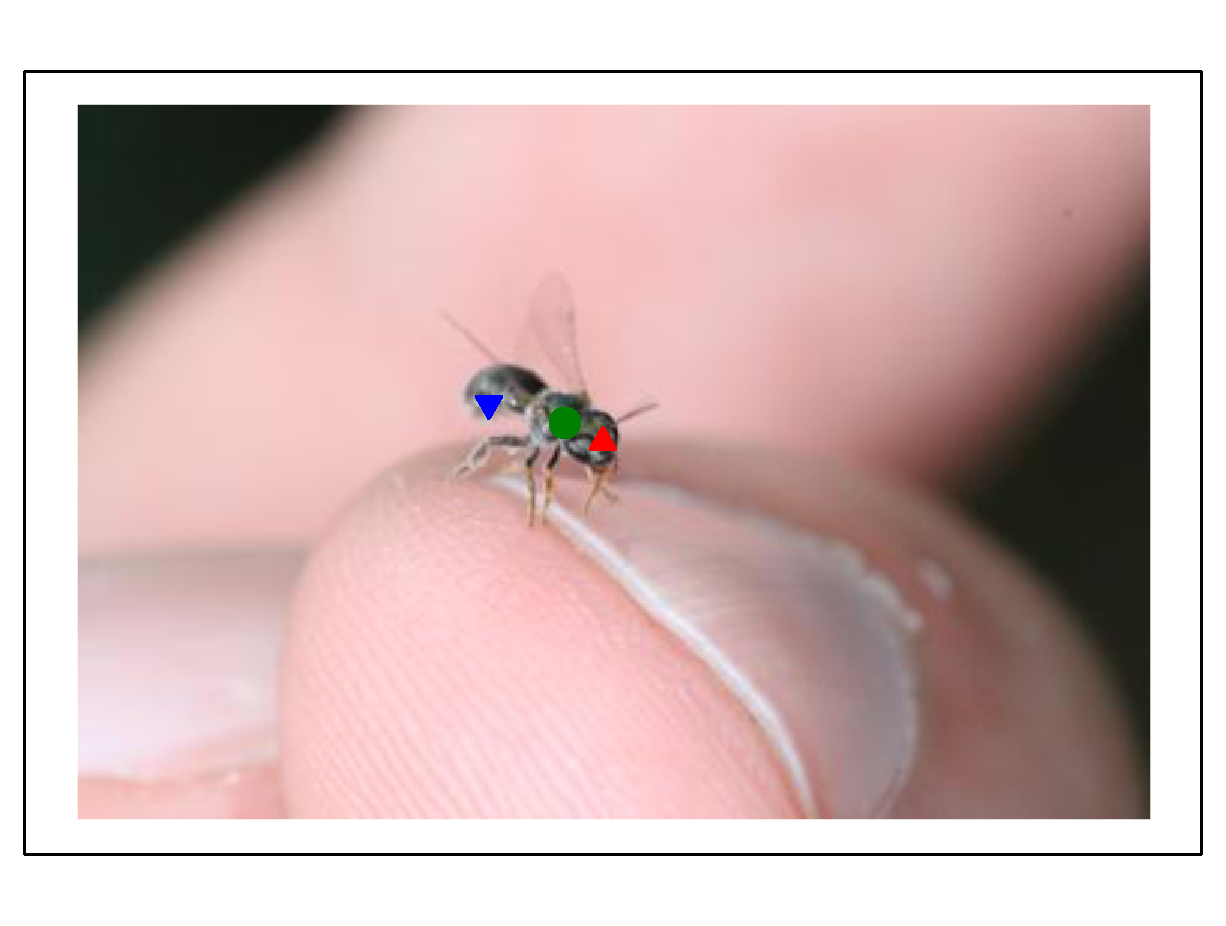
\includegraphics[width=\textwidth]{hog5_2.pdf}
                \caption{$5\times5$ HOG cells}
            \end{subfigure}
            \begin{subfigure}[b]{0.3\textwidth}
                \centering
                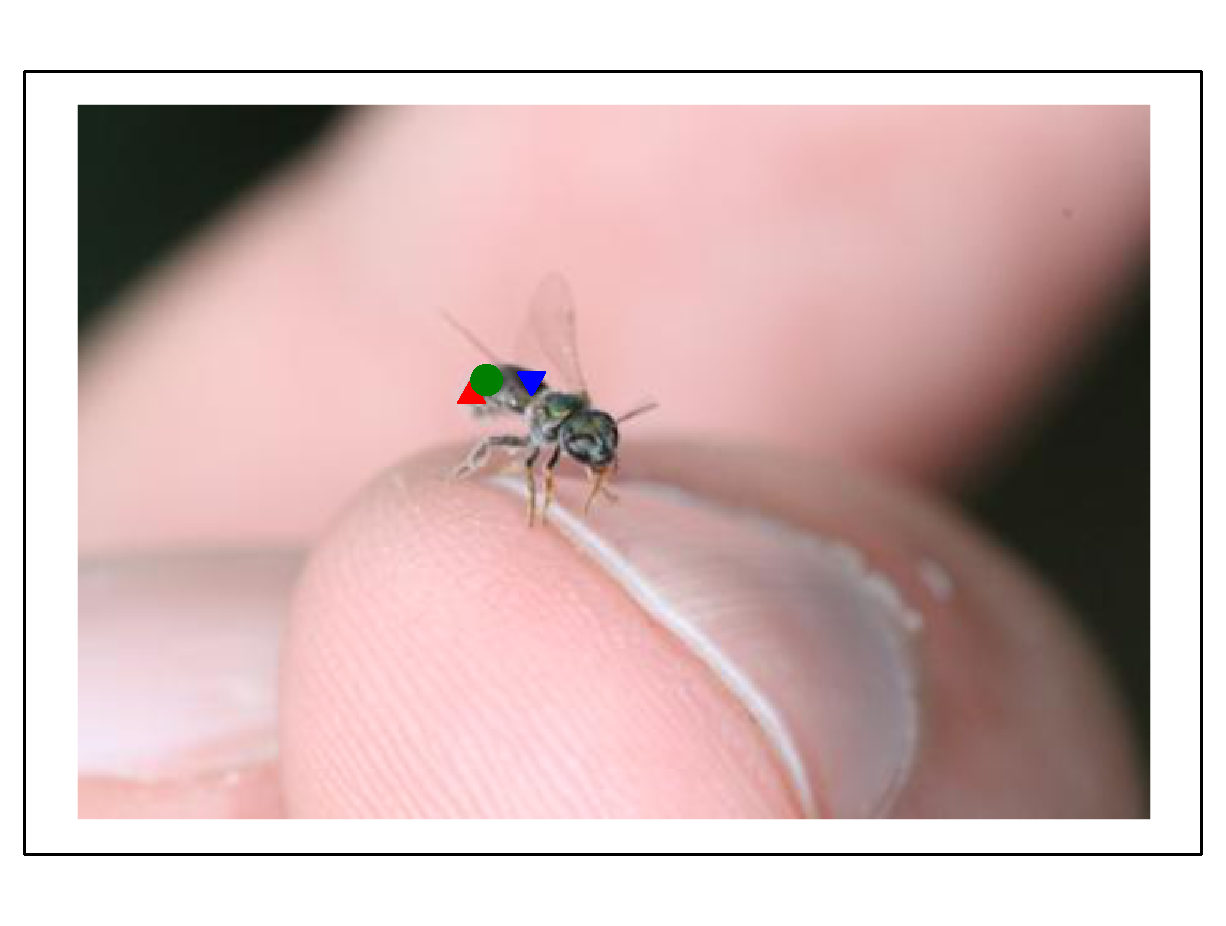
\includegraphics[width=\textwidth]{hog6_2.pdf}
                \caption{$6\times6$ HOG cells}
            \end{subfigure}
            \begin{subfigure}[b]{0.3\textwidth}
                \centering
                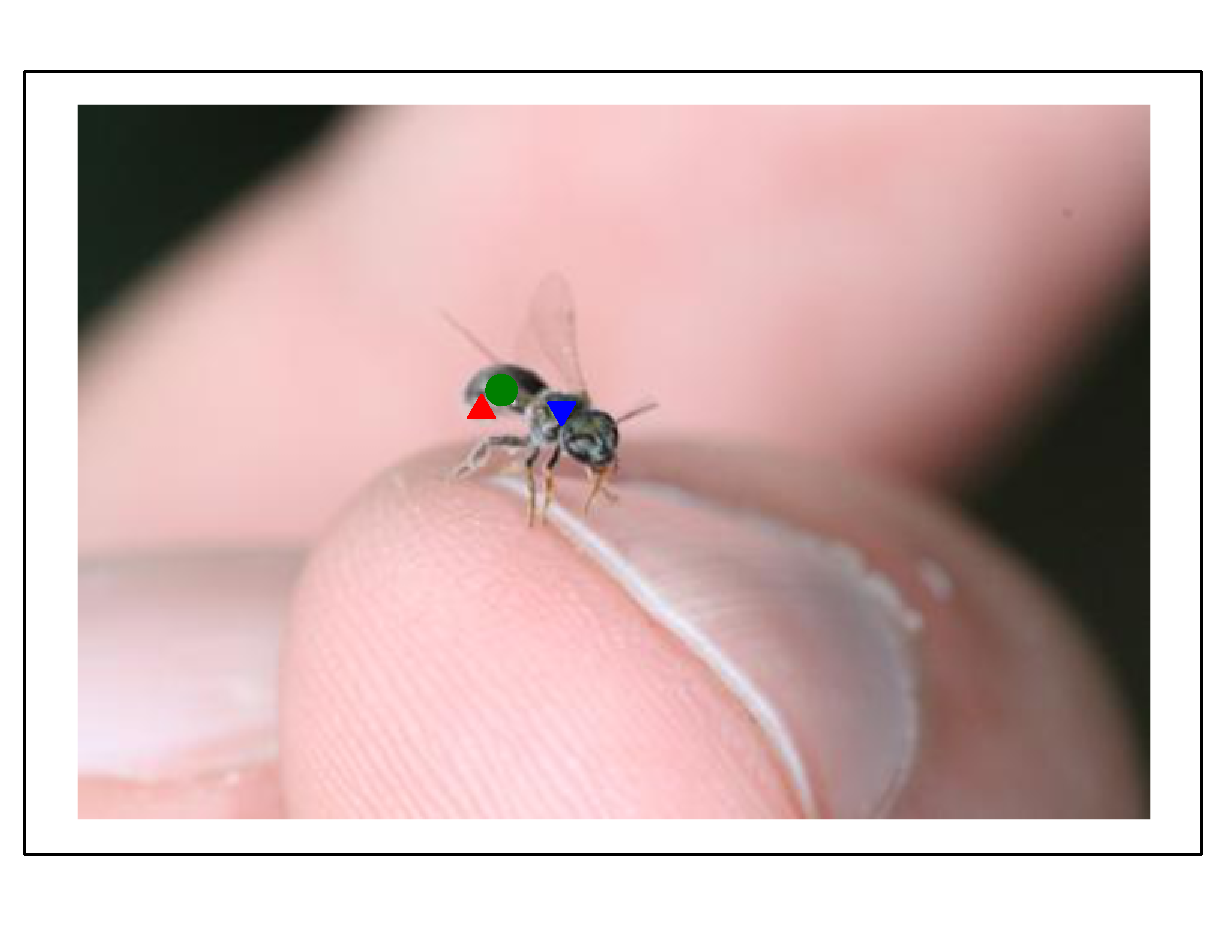
\includegraphics[width=\textwidth]{hog8_2.pdf}
                \caption{$8\times8$ HOG cells}
            \end{subfigure}
            \begin{subfigure}[b]{0.3\textwidth}
                \centering
                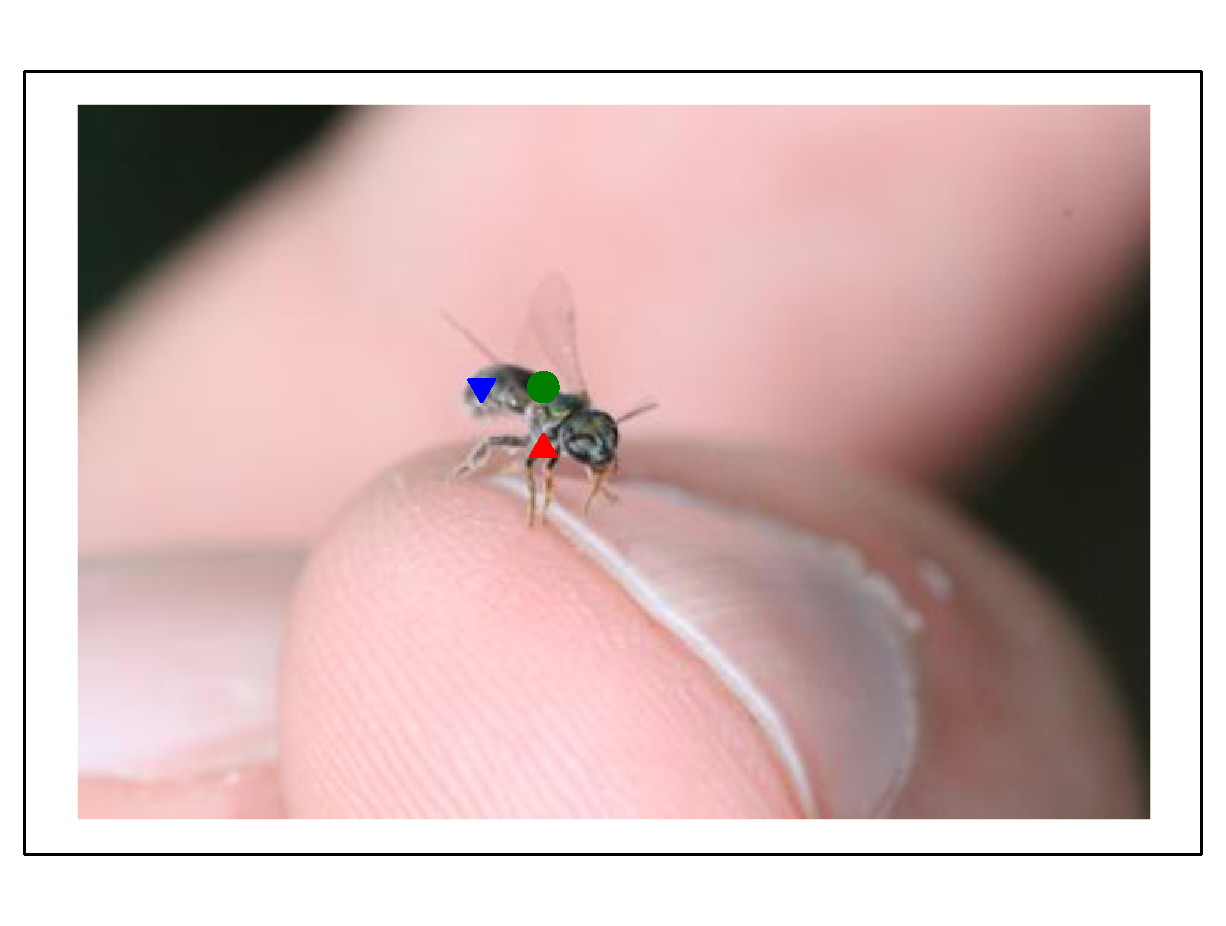
\includegraphics[width=\textwidth]{hog10_2.pdf}
                \caption{$10\times10$ HOG cells}
            \end{subfigure}
            \begin{subfigure}[b]{0.3\textwidth}
                \centering
                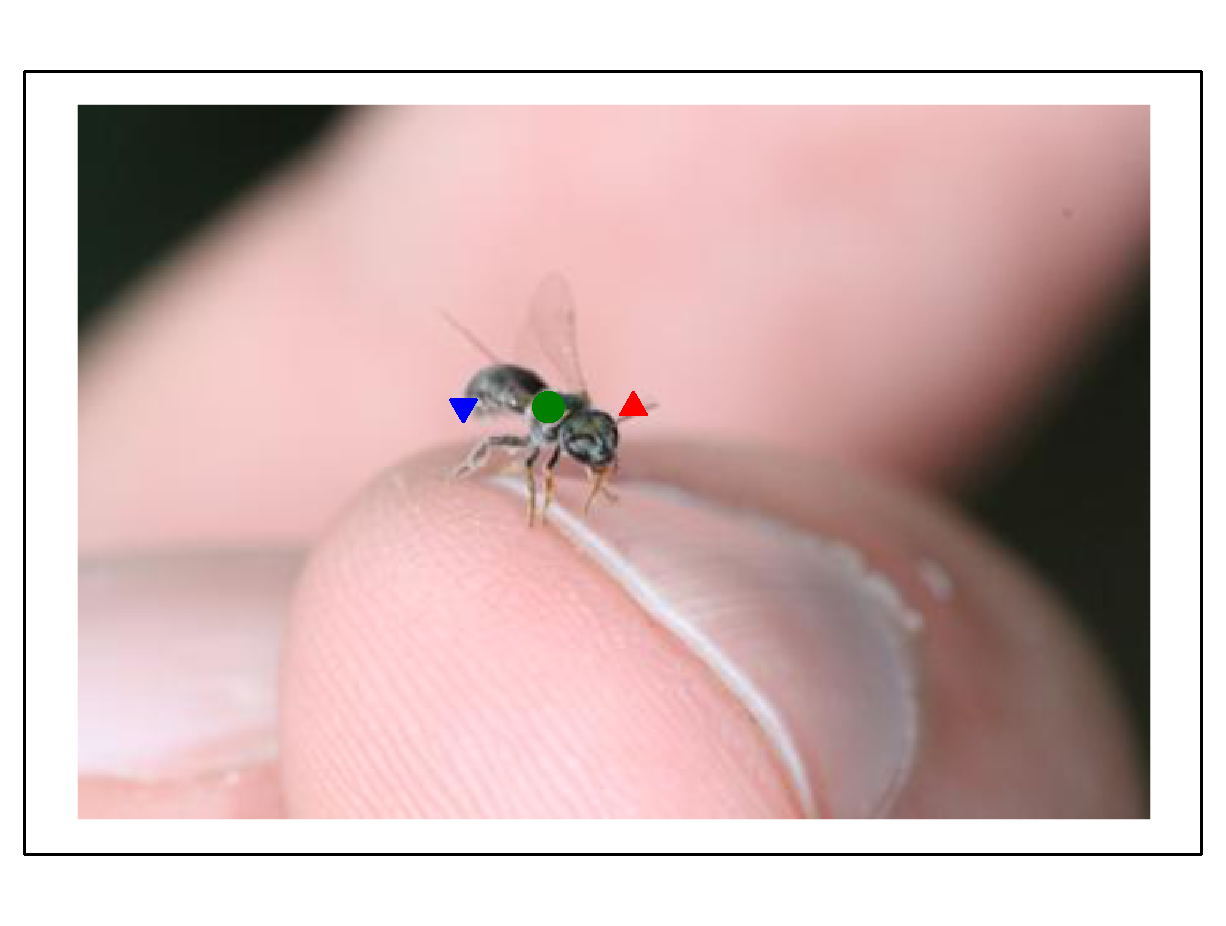
\includegraphics[width=\textwidth]{hog12_2.pdf}
                \caption{$12\times12$ HOG cells}
            \end{subfigure}
            \begin{subfigure}[b]{0.3\textwidth}
                \centering
                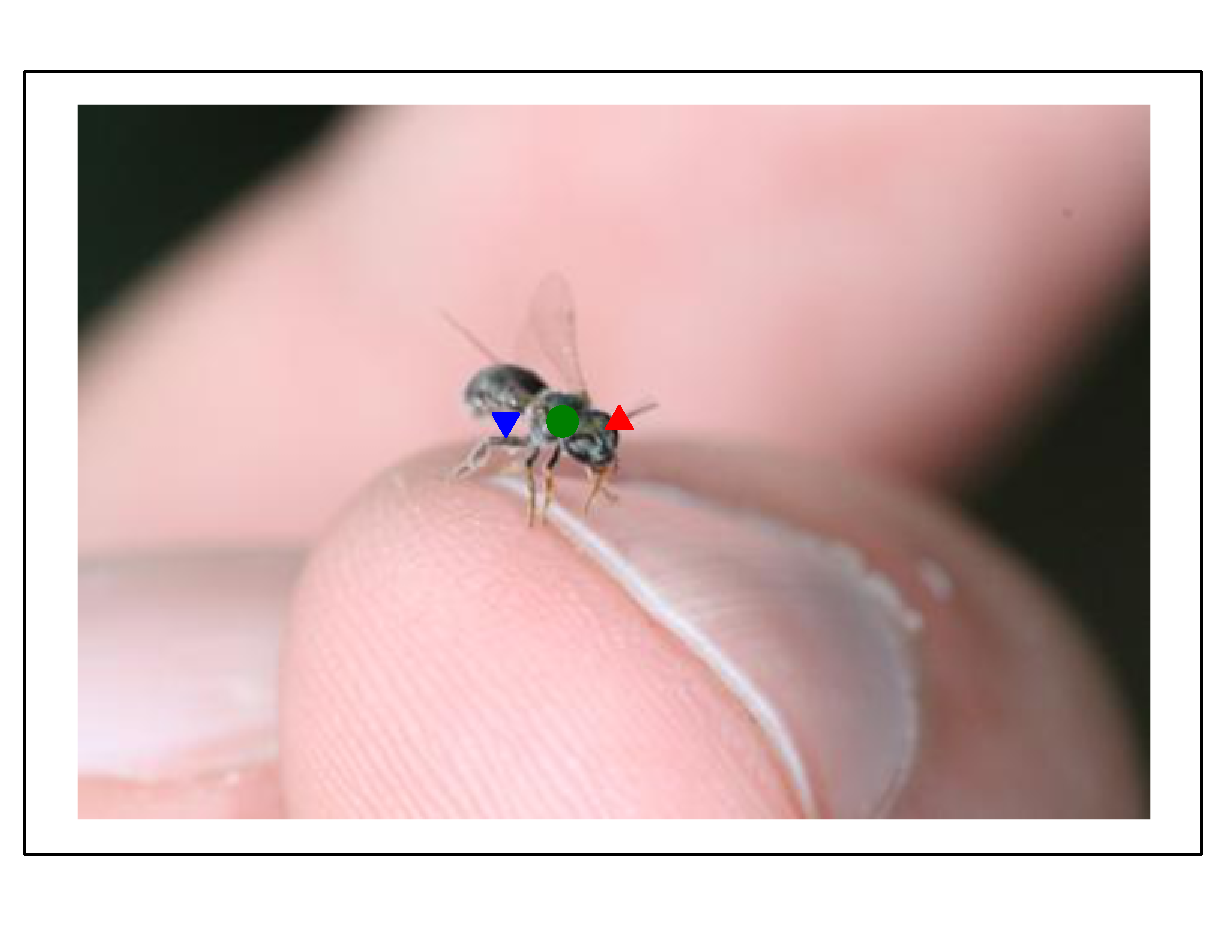
\includegraphics[width=\textwidth]{hog16_2.pdf}
                \caption{$16\times16$ HOG cells}
            \end{subfigure}
            \begin{subfigure}[b]{0.3\textwidth}
                \centering
                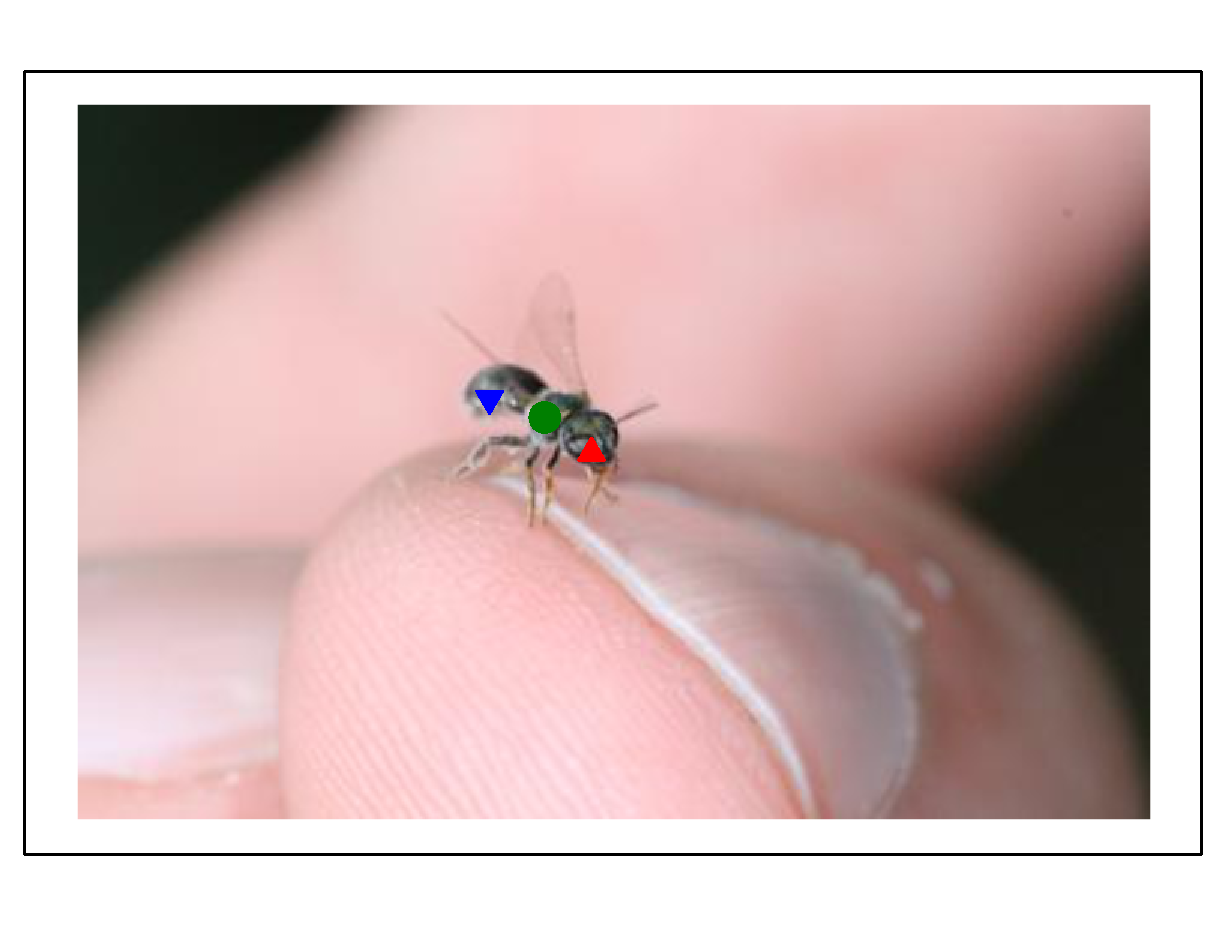
\includegraphics[width=\textwidth]{hog_gt2.pdf}
                \caption{Ground truth}
            \end{subfigure}

            \hspace{0pt}

            \begin{subfigure}[b]{0.2\textwidth}
                \centering
                \fbox{\begin{minipage}{\textwidth}
                    \begin{tabular}{c l}
                    {\legends\color{red}{\rotatebox[origin=c]{0}{▲}}}&Head\\
                    {\legends\color{green}{●}}&Thorax\\
                    {\legends\color{blue}{\rotatebox[origin=c]{180}{▲}}}&Abdomen
                    \end{tabular}
                \end{minipage}}
            \end{subfigure}
            \caption{Three-part model predictions on sample test image by HOG cell size}
            \label{fig:hog_vis2}
        \end{figure}

        \begin{figure}[p]
            \centering
            \begin{subfigure}[b]{0.3\textwidth}
                \centering
                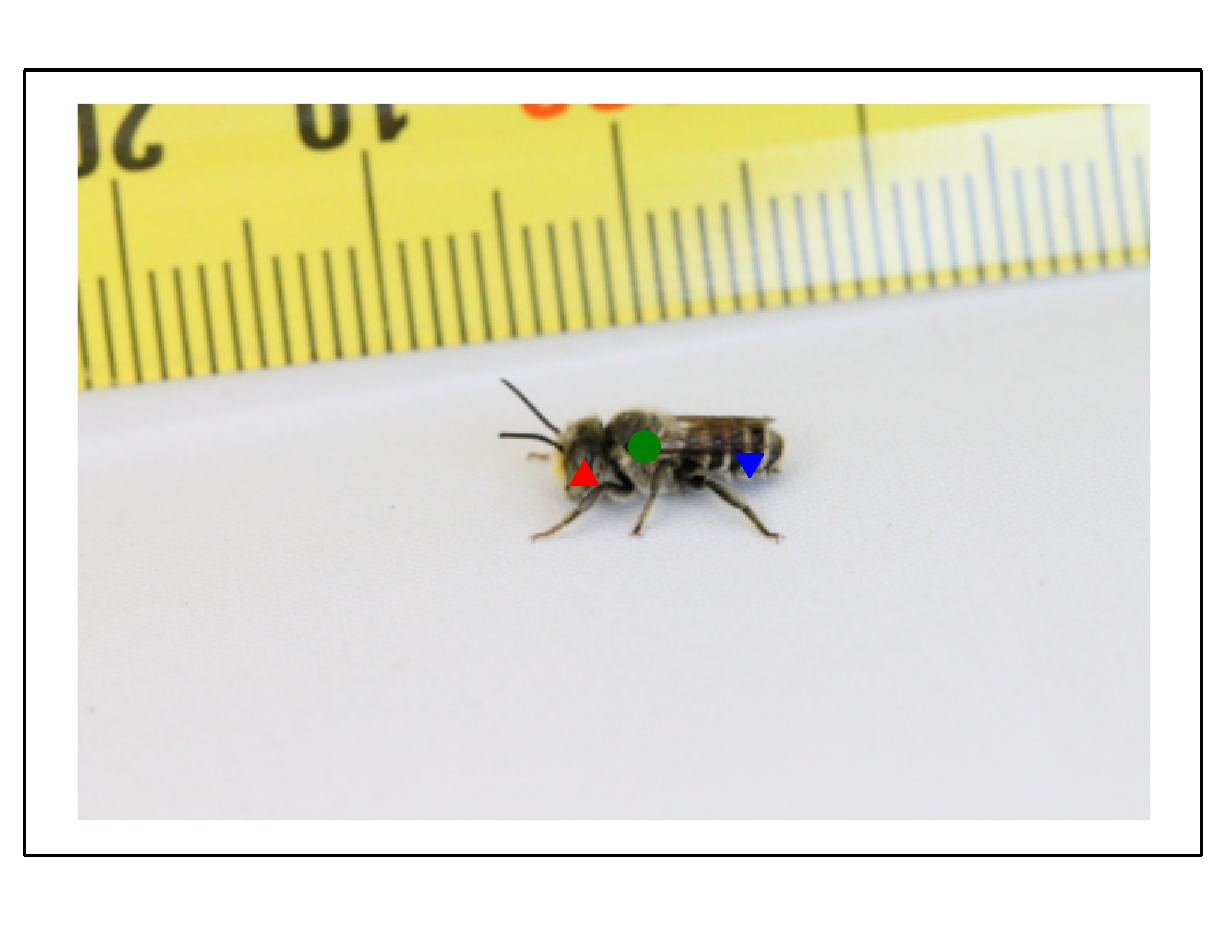
\includegraphics[width=\textwidth]{hog3_3.pdf}
                \caption{$3\times3$ HOG cells}
            \end{subfigure}
            \begin{subfigure}[b]{0.3\textwidth}
                \centering
                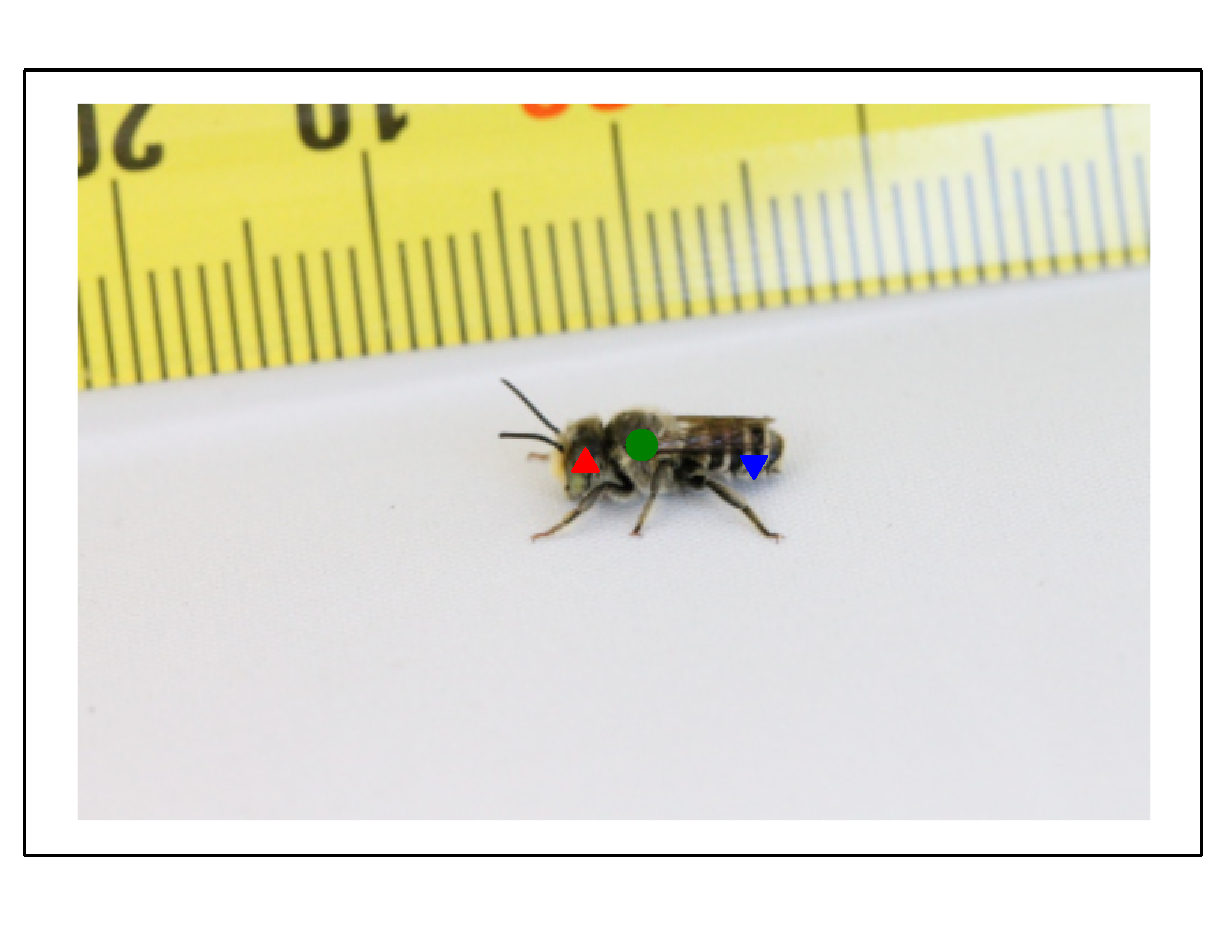
\includegraphics[width=\textwidth]{hog4_3.pdf}
                \caption{$4\times4$ HOG cells}
            \end{subfigure}
            \begin{subfigure}[b]{0.3\textwidth}
                \centering
                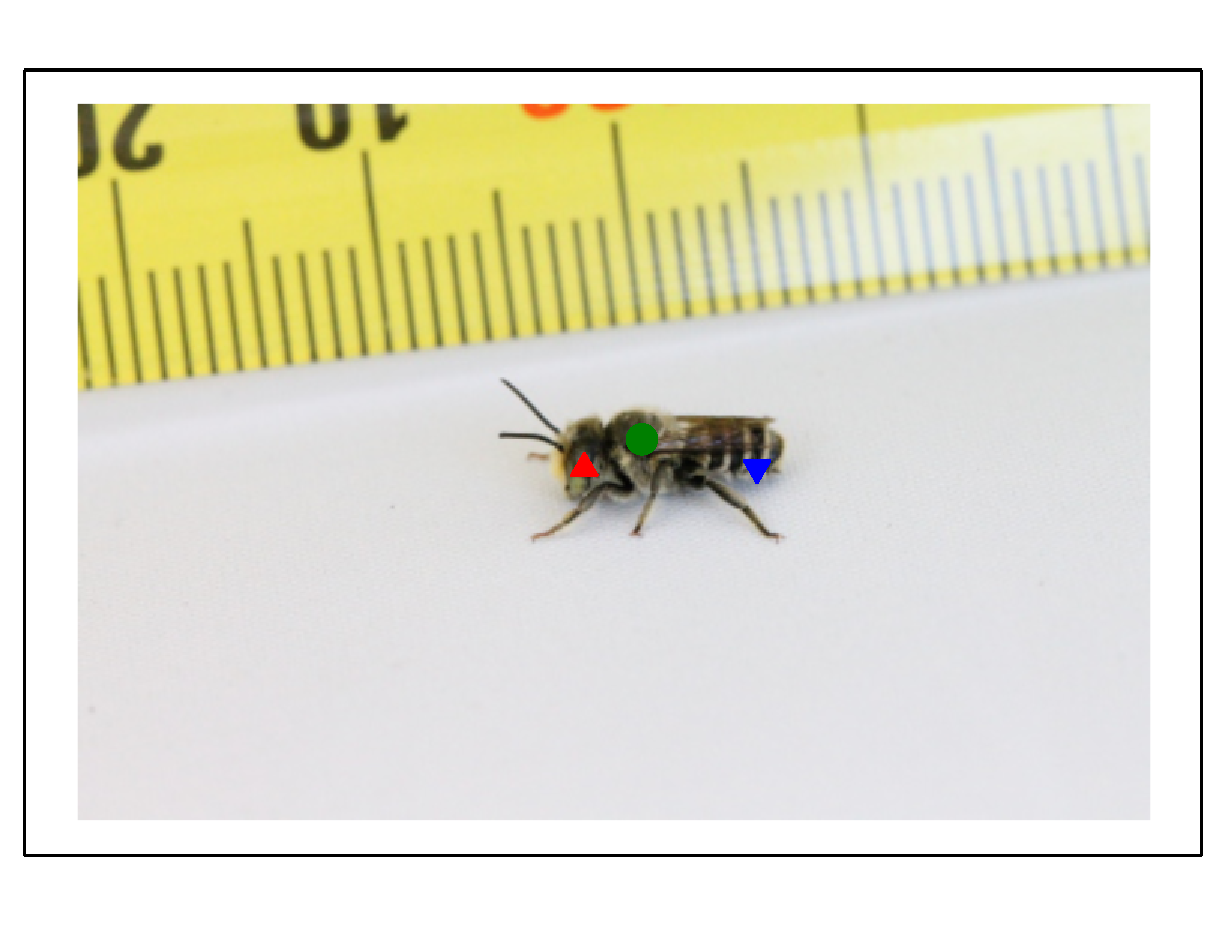
\includegraphics[width=\textwidth]{hog5_3.pdf}
                \caption{$5\times5$ HOG cells}
            \end{subfigure}
            \begin{subfigure}[b]{0.3\textwidth}
                \centering
                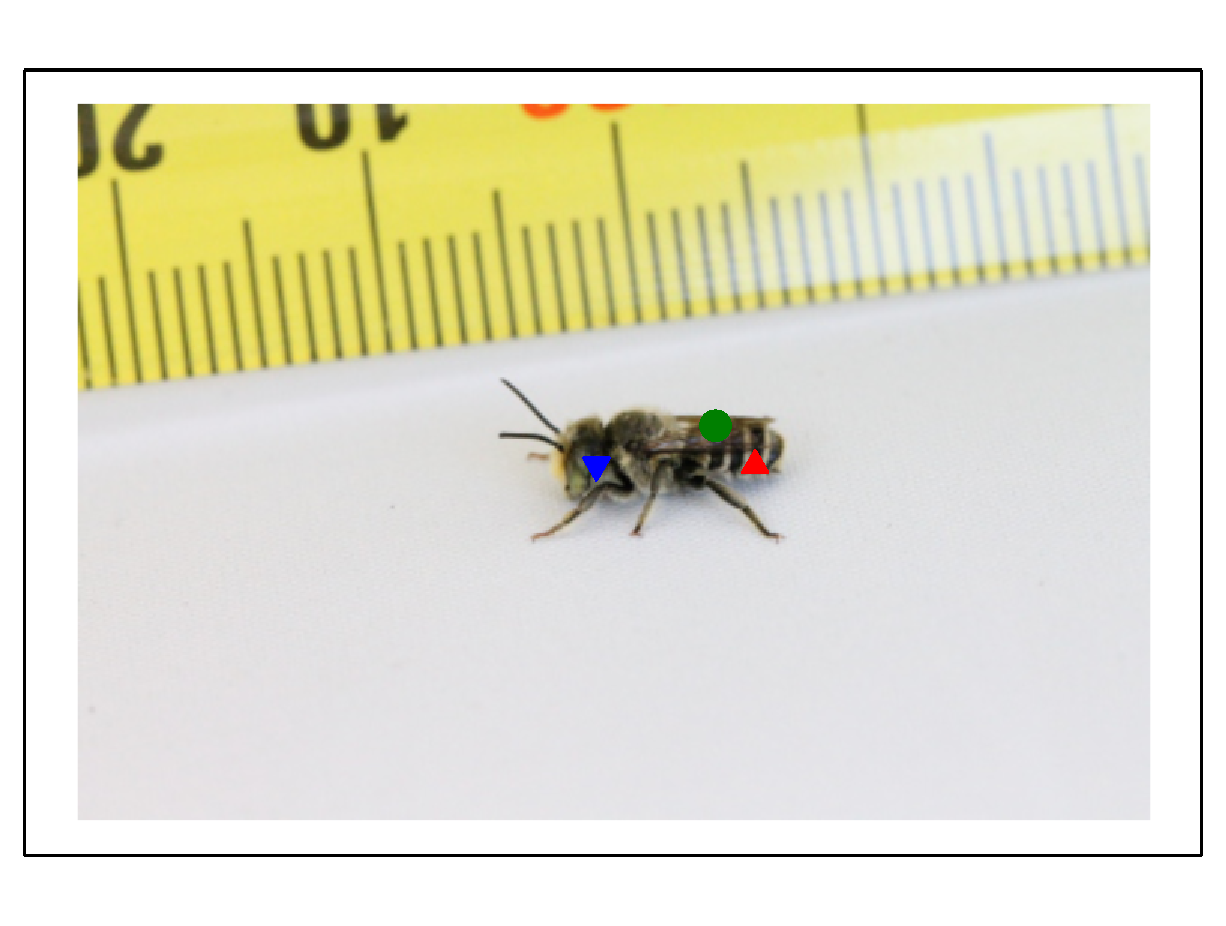
\includegraphics[width=\textwidth]{hog6_3.pdf}
                \caption{$6\times6$ HOG cells}
            \end{subfigure}
            \begin{subfigure}[b]{0.3\textwidth}
                \centering
                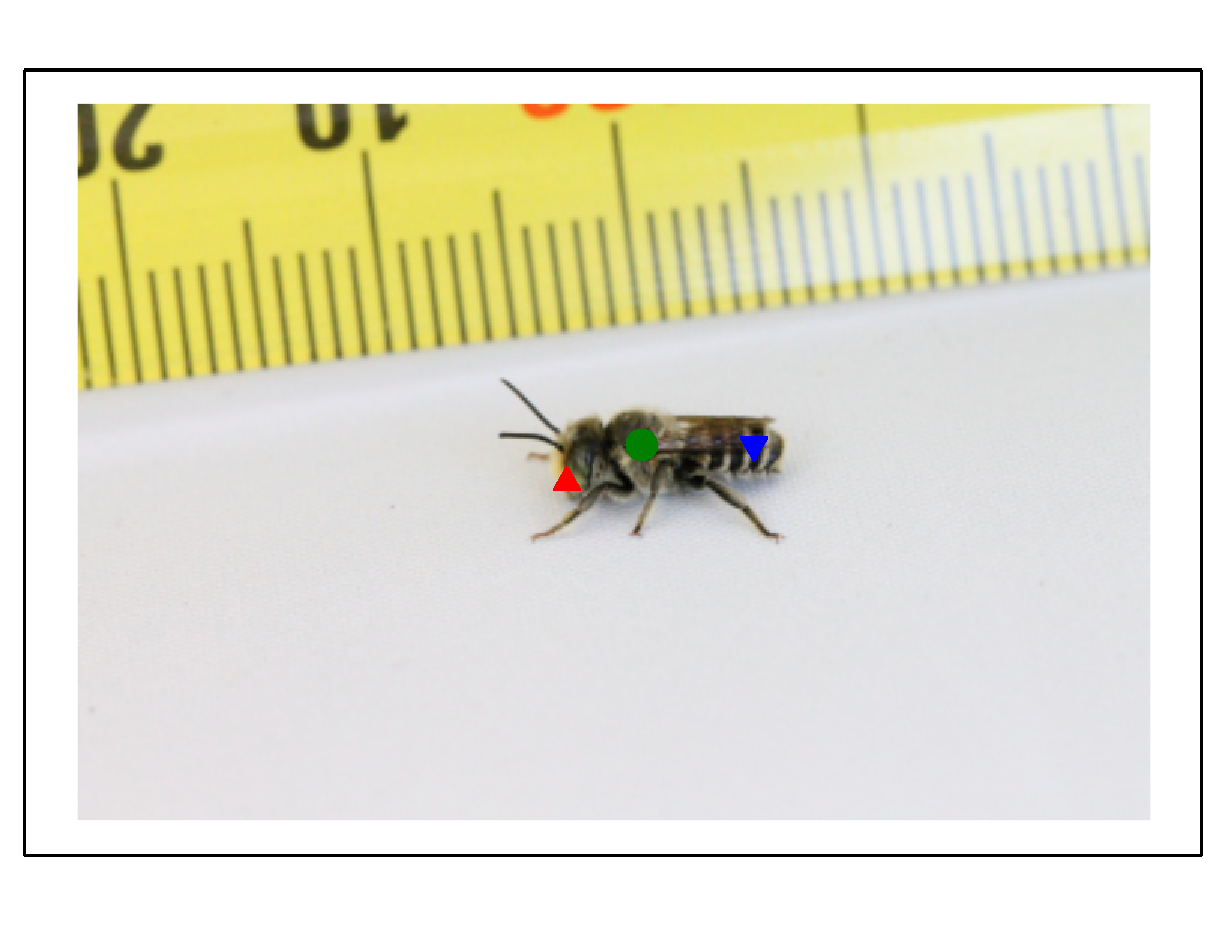
\includegraphics[width=\textwidth]{hog8_3.pdf}
                \caption{$8\times8$ HOG cells}
            \end{subfigure}
            \begin{subfigure}[b]{0.3\textwidth}
                \centering
                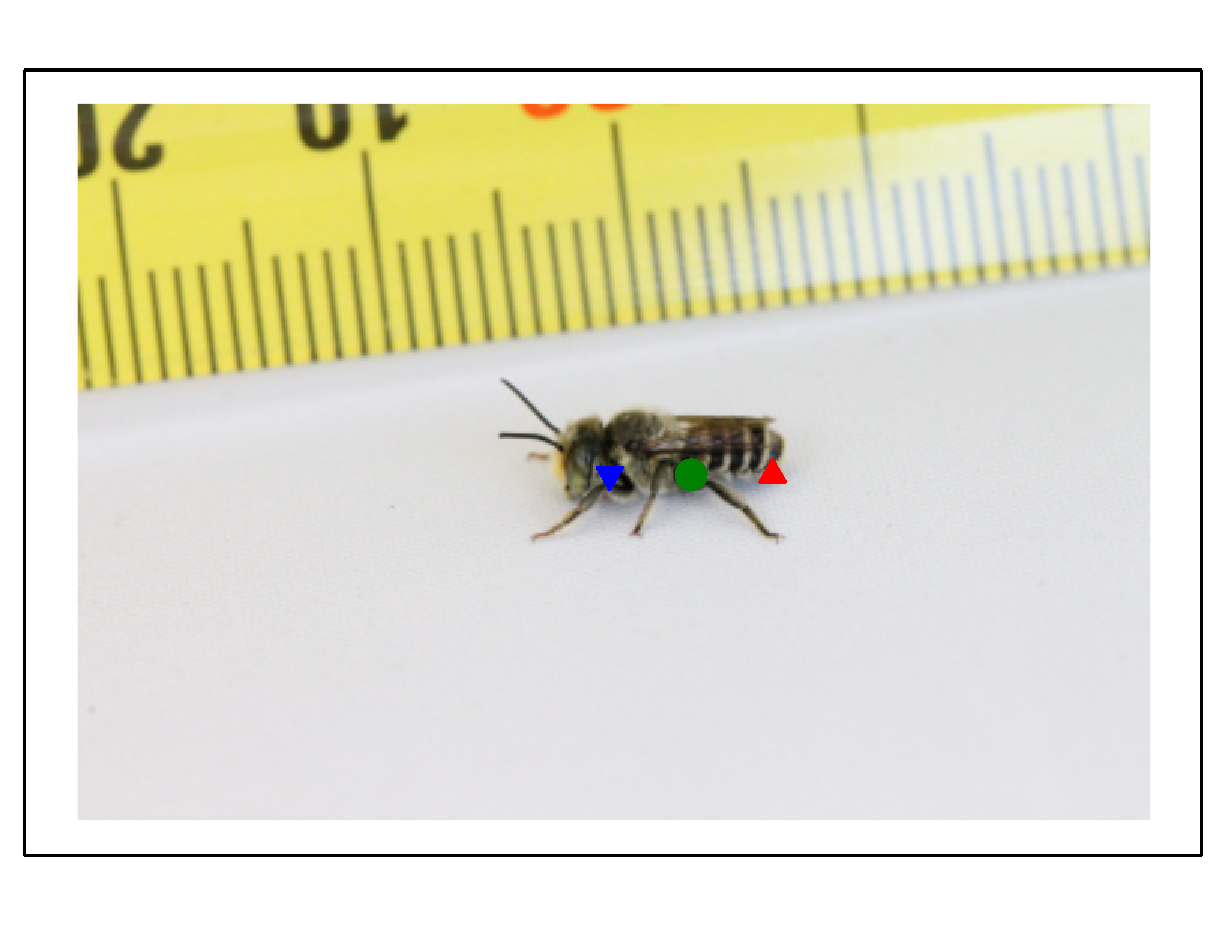
\includegraphics[width=\textwidth]{hog10_3.pdf}
                \caption{$10\times10$ HOG cells}
            \end{subfigure}
            \begin{subfigure}[b]{0.3\textwidth}
                \centering
                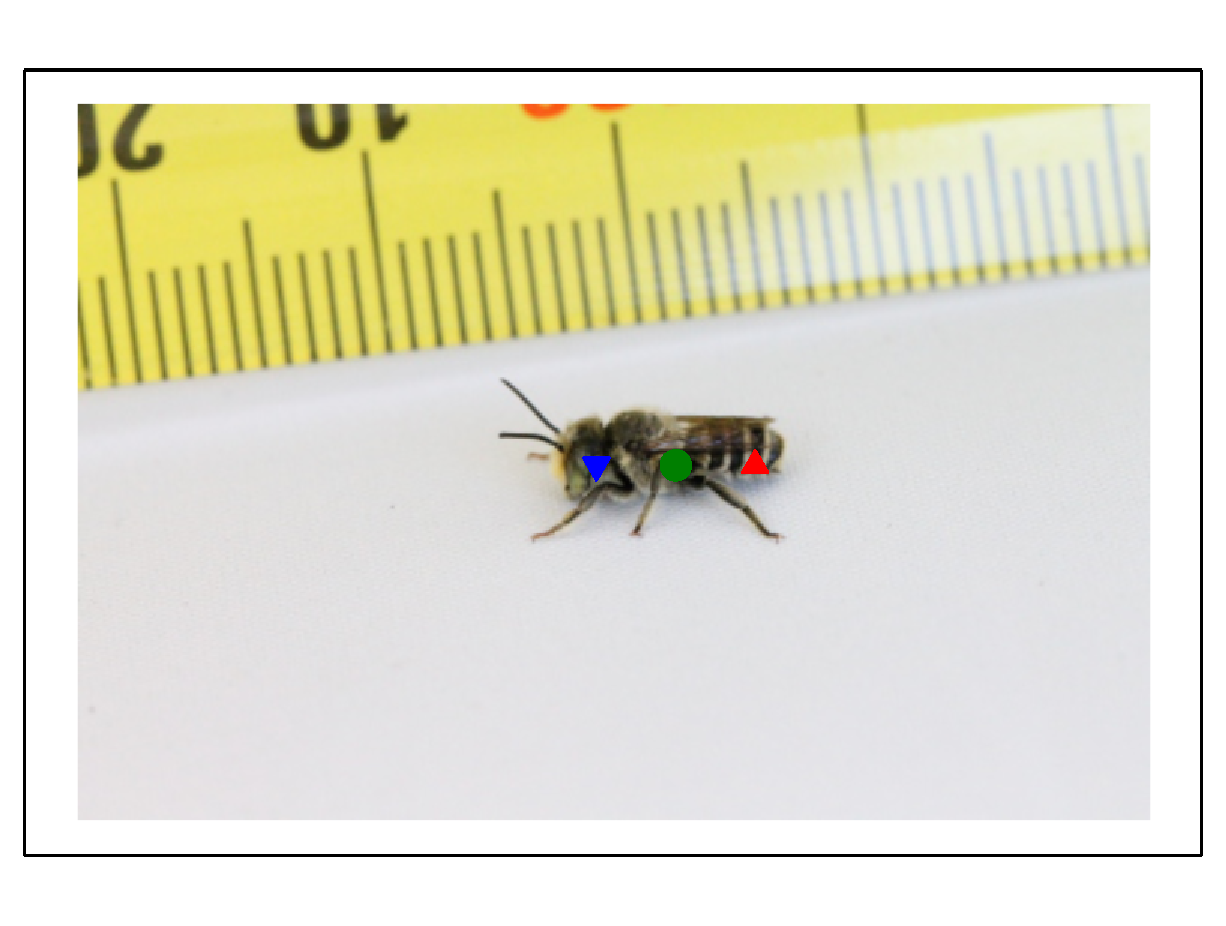
\includegraphics[width=\textwidth]{hog12_3.pdf}
                \caption{$12\times12$ HOG cells}
            \end{subfigure}
            \begin{subfigure}[b]{0.3\textwidth}
                \centering
                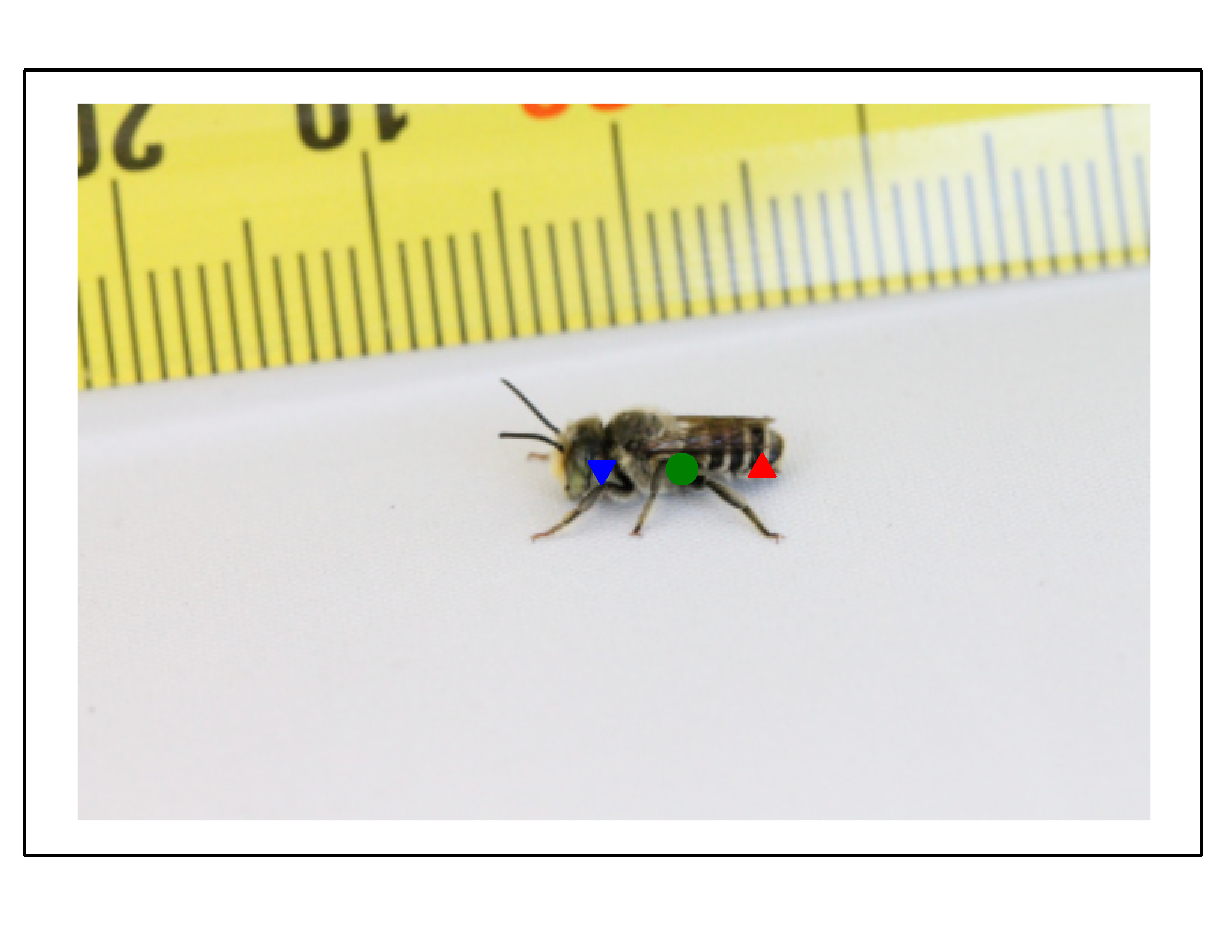
\includegraphics[width=\textwidth]{hog16_3.pdf}
                \caption{$16\times16$ HOG cells}
            \end{subfigure}
            \begin{subfigure}[b]{0.3\textwidth}
                \centering
                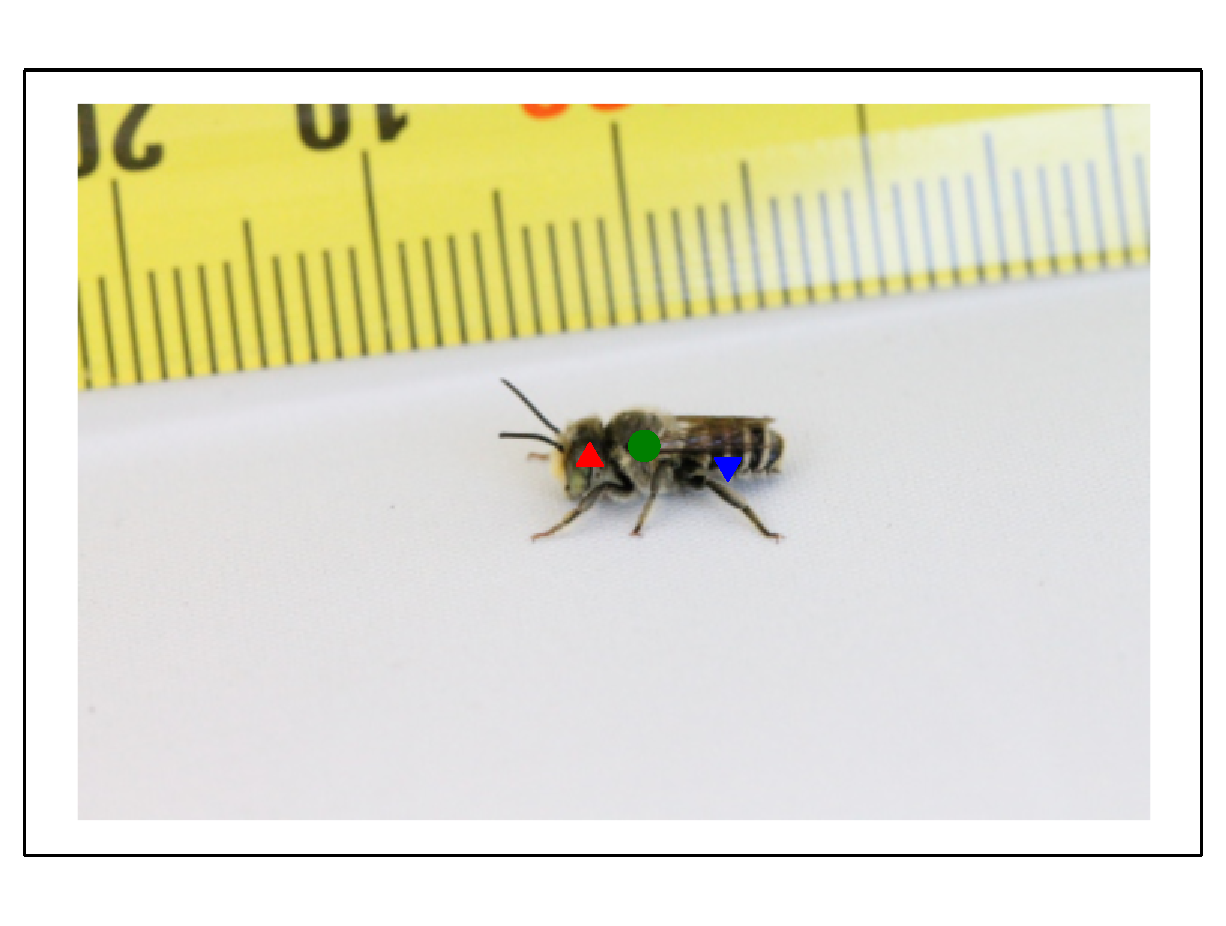
\includegraphics[width=\textwidth]{hog_gt3.pdf}
                \caption{Ground truth}
            \end{subfigure}

            \hspace{0pt}

            \begin{subfigure}[b]{0.2\textwidth}
                \centering
                \fbox{\begin{minipage}{\textwidth}
                    \begin{tabular}{c l}
                    {\legends\color{red}{\rotatebox[origin=c]{0}{▲}}}&Head\\
                    {\legends\color{green}{●}}&Thorax\\
                    {\legends\color{blue}{\rotatebox[origin=c]{180}{▲}}}&Abdomen
                    \end{tabular}
                \end{minipage}}
            \end{subfigure}
            \caption{Three-part model predictions on sample test image by HOG cell size}
            \label{fig:hog_vis3}
        \end{figure}
    \section{Comparison of three- and seven-part models}
        We compared the performace of the three part model against the seven-part model. The models were described in section 3.2.

        As visible in figures \ref{fig:37_pck} and \ref{fig:37_apk}, the seven-part model does not perform well in predicting the locations of the wings and the antennae, although the additional parts assist in predicting the locations of the head, the thorax, and the abdomen. In fact the seven-part model is clearly superior to the three-part model in predicting the locations of the parts that they share, despite its relative lack of utility in predicting the wings and the antennae.

        This may be visually confirmed by examining figures \ref{fig:37_vis1}, \ref{fig:37_vis2}, and \ref{fig:37_vis3}.

        This may be explained by antennae and wings being difficult to detect. Antennae are thin and may easily be confused with the legs of the bee. Wings are transluscent, take up a wide variety of positions, and lack uniformity. Nevertheless, those parts are still detected with some precision, though rarely exactly. That extra information assists the graphical model in determining the locations of the head, abdomen and the thorax.

        \begin{figure}
            \centering
            \begin{minipage}{0.48\textwidth}
                \centering
                    \begin{tikzpicture}
                        \begin{axis}[width=\textwidth,
                            xlabel=Number of parts in model,
                            ylabel=Probability of Correct Keypoint (\%)]
                        \addplot[only marks,color=red,mark=triangle*] coordinates {
                            ( 3, 63)
                            ( 7, 63)
                        };
                        \addplot[only marks,color=green,mark=*] coordinates {
                            ( 3, 70)
                            ( 7, 64)
                        };
                        \addplot[only marks,color=blue,mark=triangle*, mark options={rotate=180}] coordinates {
                            ( 3, 50)
                            ( 7, 56)
                        };
                        \addplot[only marks,color=cyan,mark=triangle*, mark options={rotate=90}] coordinates {
                            ( 7, 28)
                        };
                        \addplot[only marks,color=cyan,mark=triangle*, mark options={rotate=270}] coordinates {
                            ( 7, 22)
                        };
                        \addplot[only marks,color=yellow,mark=halfsquare left*] coordinates {
                            ( 7, 28)
                        };
                        \addplot[only marks,color=yellow,mark=halfsquare right*] coordinates {
                            ( 7, 25)
                        };
                        \addplot[only marks,color=black,mark=square*] coordinates {
                            ( 3, 61)
                            ( 7, 61)
                        };
                        \addplot[only marks,color=black,mark=square, mark options={rotate=180}] coordinates {
                            ( 7, 40.9)
                            (11, 60)
                        };
                        \legend{Head, Thorax, Abdomen, L Wing, R Wing, L Antenna, R Antenna, Mean (3p), Mean (7p)}
                        \end{axis}
                    \end{tikzpicture}
                \caption{PCK by parts in model for HOG cell size 4}
                \label{fig:37_pck}
            \end{minipage}\hfill
            \begin{minipage}{0.48\textwidth}
                \centering
                \begin{tikzpicture}
                    \begin{axis}[width=\textwidth,
                        xlabel=Number of parts in model,
                        ylabel=Average Precision of Keypoints (\%)]
                    \addplot[only marks,color=red,mark=triangle*] coordinates {
                            ( 3, 56.2)
                            ( 7, 66.5)
                        };
                        \addplot[only marks,color=green,mark=*] coordinates {
                            ( 3, 56.2)
                            ( 7, 62.2)
                        };
                        \addplot[only marks,color=blue,mark=triangle*, mark options={rotate=180}] coordinates {
                            ( 3, 46.5)
                            ( 7, 51.2)
                        };
                        \addplot[only marks,color=cyan,mark=triangle*, mark options={rotate=90}] coordinates {
                            ( 7, 11)
                        };
                        \addplot[only marks,color=cyan,mark=triangle*, mark options={rotate=270}] coordinates {
                            ( 7, 9)
                        };
                        \addplot[only marks,color=yellow,mark=halfsquare left*] coordinates {
                            ( 7, 17)
                        };
                        \addplot[only marks,color=yellow,mark=halfsquare right*] coordinates {
                            ( 7, 18.4)
                        };
                        \addplot[only marks,color=black,mark=square*] coordinates {
                            ( 3, 53)
                            ( 7, 60)
                        };
                        \addplot[only marks,color=black,mark=square, mark options={rotate=180}] coordinates {
                            ( 7, 33.6)
                            (11, 60)
                        };
                        \legend{Head, Thorax, Abdomen, L Wing, R Wing, L Antenna, R Antenna, Mean (3p), Mean (7p)}
                    \end{axis}
                \end{tikzpicture}
                \caption{APK by parts in model for HOG cell size 4}
                \label{fig:37_apk}
            \end{minipage}
        \end{figure}

        \begin{figure}[p]
            \centering
            \begin{subfigure}[b]{0.45\textwidth}
                \centering
                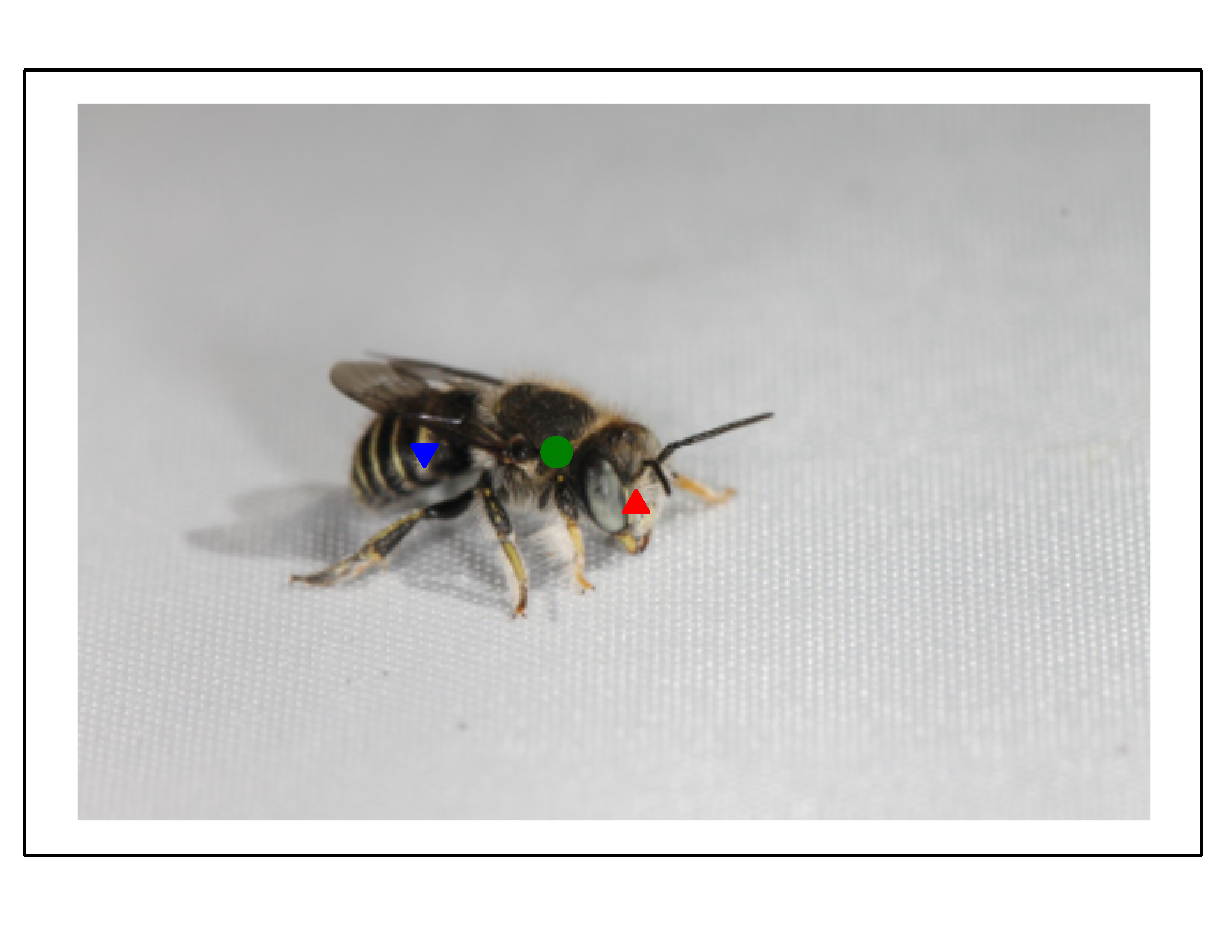
\includegraphics[width=\textwidth]{hog4_1.pdf}
                \caption{Three-part model}
            \end{subfigure}
            \begin{subfigure}[b]{0.45\textwidth}
                \centering
                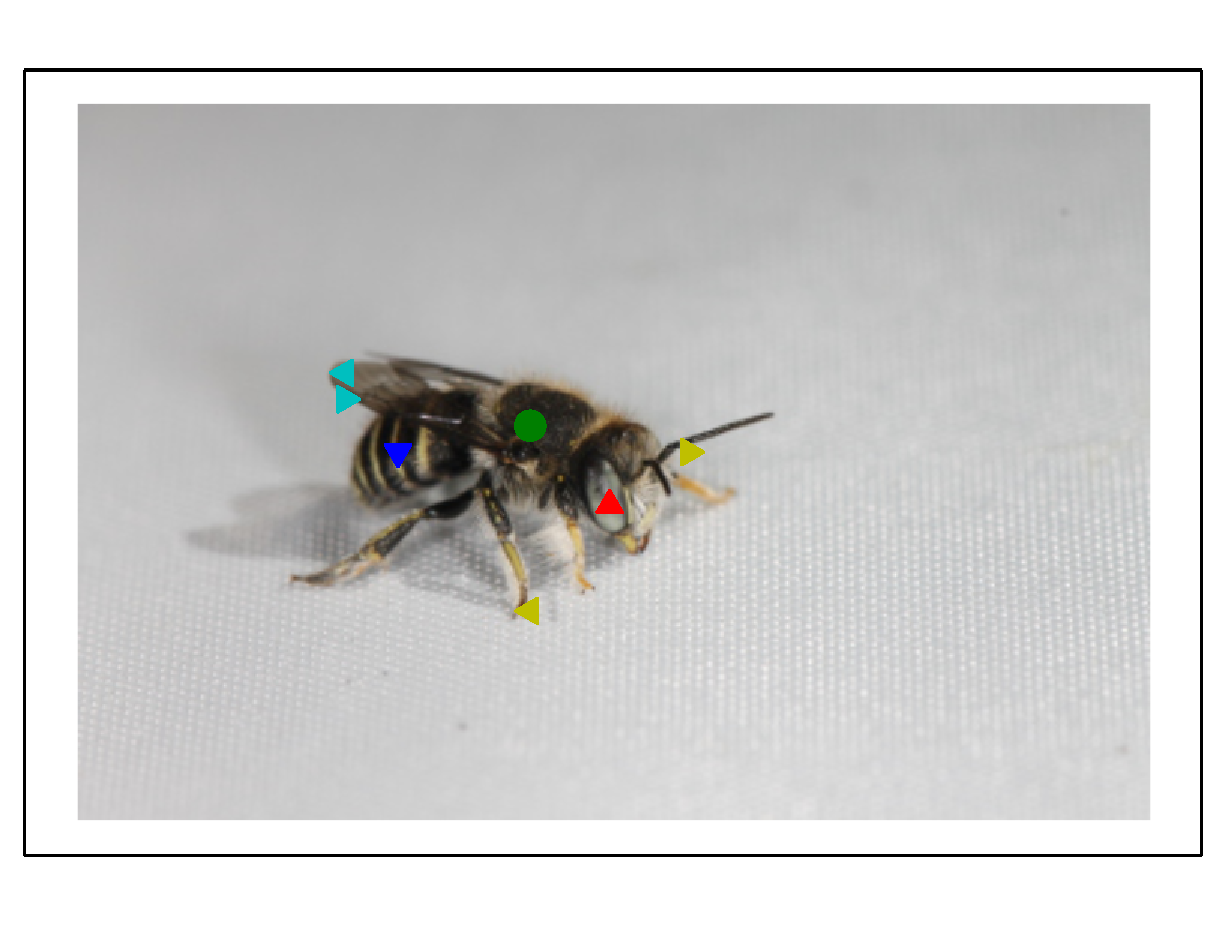
\includegraphics[width=\textwidth]{7p_1.pdf}
                \caption{Seven-part model}
            \end{subfigure}
            \begin{subfigure}[b]{0.45\textwidth}
                \centering
                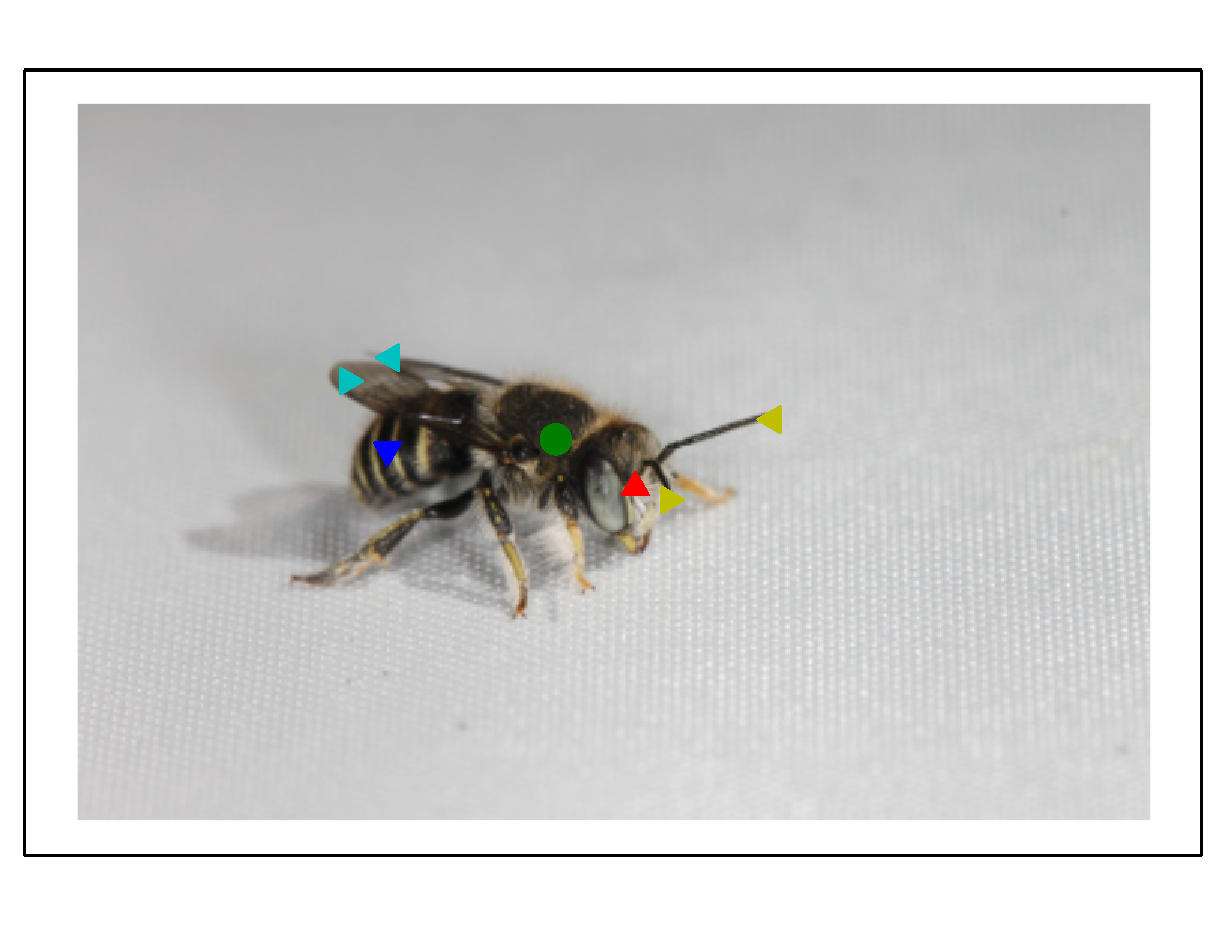
\includegraphics[width=\textwidth]{7pgt_1.pdf}
                \caption{Ground truth}
            \end{subfigure}
            \hspace{0.1\textwidth}\raisebox{15ex}{\framebox[0.25\textwidth]{
                \begin{tabular}{c l}
                {\legends\color{red}{\rotatebox[origin=c]{0}{▲}}}&Head\\
                {\legends\color{green}{●}}&Thorax\\
                {\legends\color{blue}{\rotatebox[origin=c]{180}{▲}}}&Abdomen\\
                {\legends\color{cyan}{\rotatebox[origin=c]{90}{▲}}}&Left Wing\\
                {\legends\color{cyan}{\rotatebox[origin=c]{270}{▲}}}&Right Wing\\
                {\legends\color{yellow}{\rotatebox[origin=c]{90}{▲}}}&Left Antenna\\
                {\legends\color{yellow}{\rotatebox[origin=c]{270}{▲}}}&Right Antenna
                \end{tabular}
            }}\hspace{0.1\textwidth}
            \caption{Predictions on sample test image by number of parts in model}
            \label{fig:37_vis1}
        \end{figure}

        \begin{figure}[p]
            \centering
            \begin{subfigure}[b]{0.45\textwidth}
                \centering
                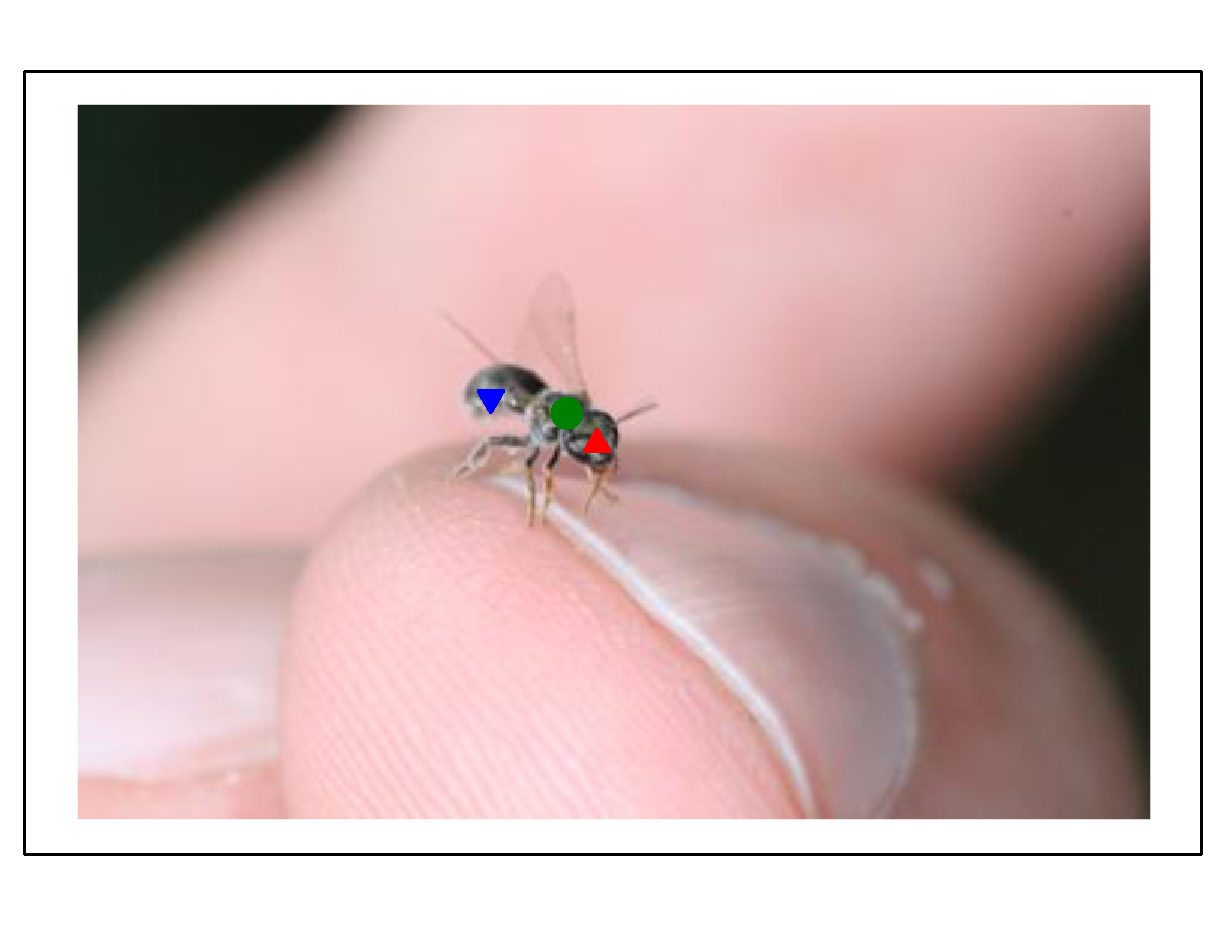
\includegraphics[width=\textwidth]{hog4_2.pdf}
                \caption{Three-part model}
            \end{subfigure}
            \begin{subfigure}[b]{0.45\textwidth}
                \centering
                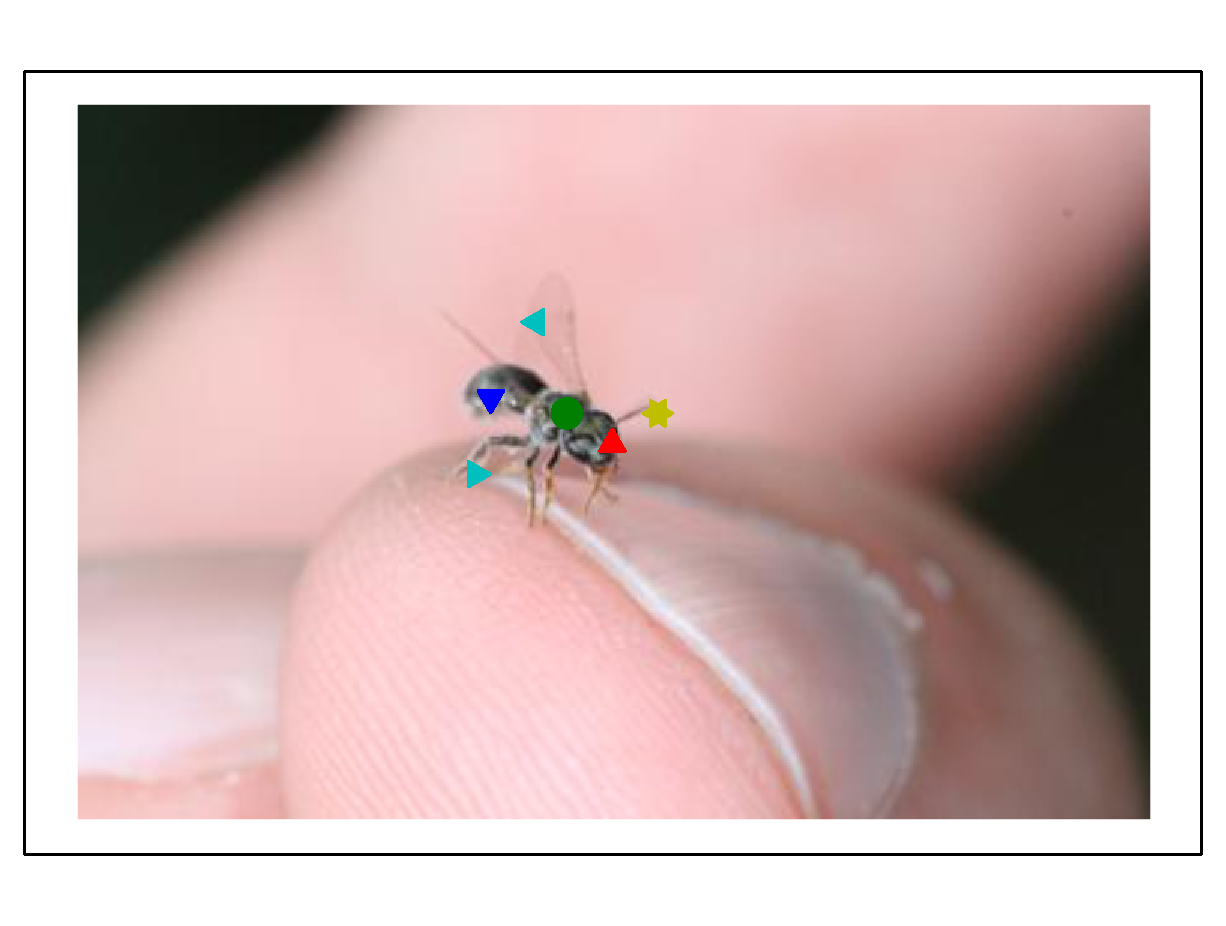
\includegraphics[width=\textwidth]{7p_2.pdf}
                \caption{Seven-part model}
            \end{subfigure}
            \begin{subfigure}[b]{0.45\textwidth}
                \centering
                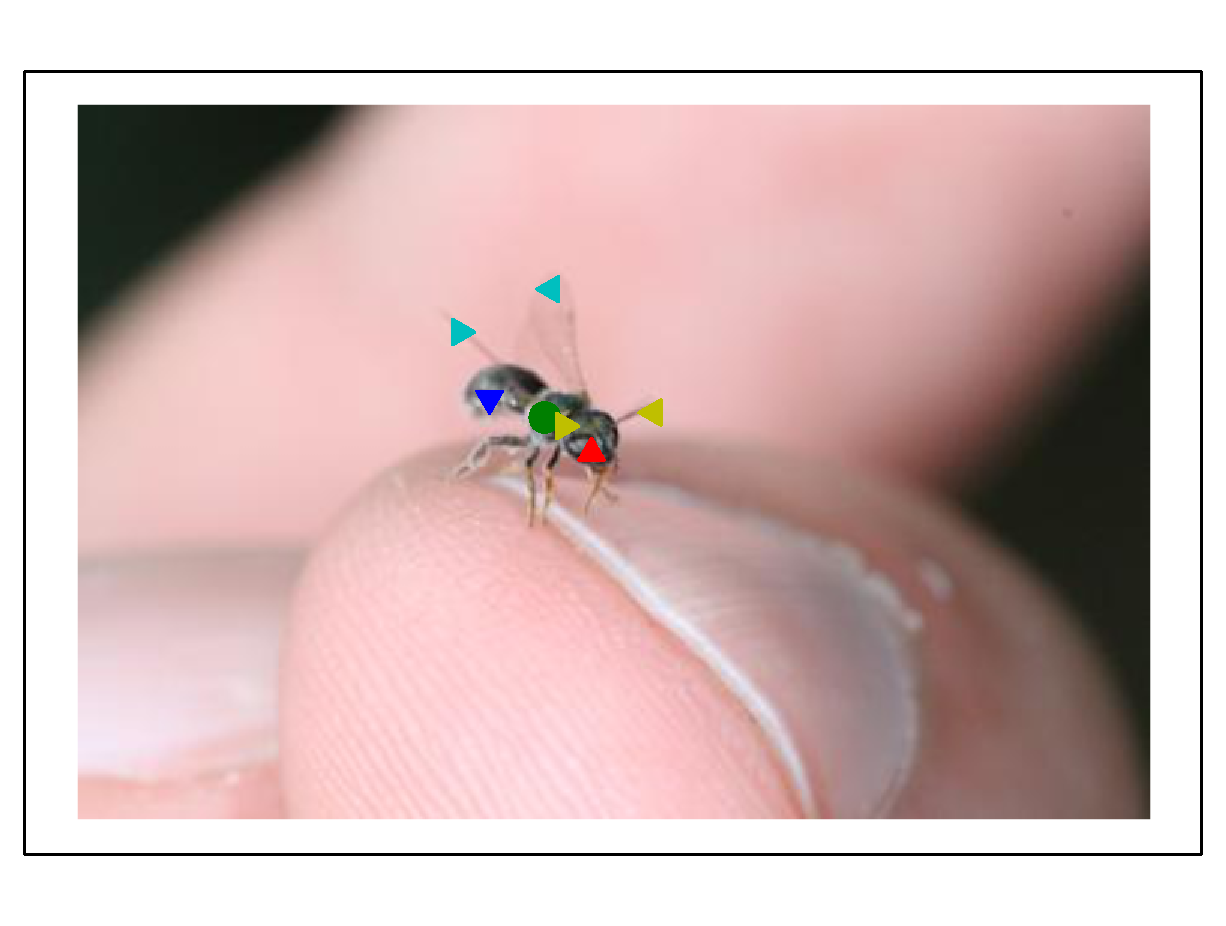
\includegraphics[width=\textwidth]{7pgt_2.pdf}
                \caption{Ground truth}
            \end{subfigure}
            \hspace{0.1\textwidth}\raisebox{15ex}{\framebox[0.25\textwidth]{
                \begin{tabular}{c l}
                {\legends\color{red}{\rotatebox[origin=c]{0}{▲}}}&Head\\
                {\legends\color{green}{●}}&Thorax\\
                {\legends\color{blue}{\rotatebox[origin=c]{180}{▲}}}&Abdomen\\
                {\legends\color{cyan}{\rotatebox[origin=c]{90}{▲}}}&Left Wing\\
                {\legends\color{cyan}{\rotatebox[origin=c]{270}{▲}}}&Right Wing\\
                {\legends\color{yellow}{\rotatebox[origin=c]{90}{▲}}}&Left Antenna\\
                {\legends\color{yellow}{\rotatebox[origin=c]{270}{▲}}}&Right Antenna
                \end{tabular}
            }}\hspace{0.1\textwidth}
            \caption{Predictions on sample test image by number of parts in model}
            \label{fig:37_vis2}
        \end{figure}

        \begin{figure}[p]
            \centering
            \begin{subfigure}[b]{0.45\textwidth}
                \centering
                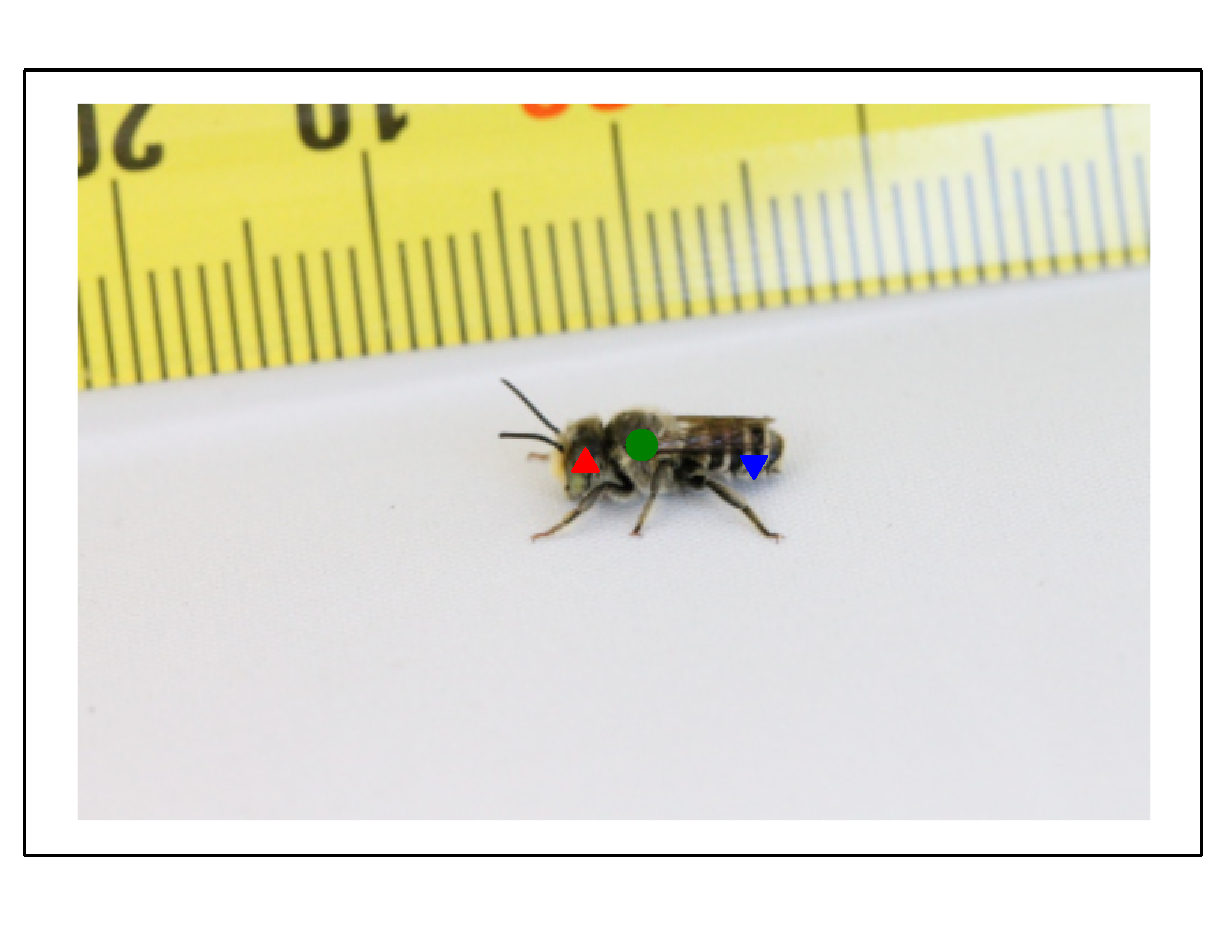
\includegraphics[width=\textwidth]{hog4_3.pdf}
                \caption{Three-part model}
            \end{subfigure}
            \begin{subfigure}[b]{0.45\textwidth}
                \centering
                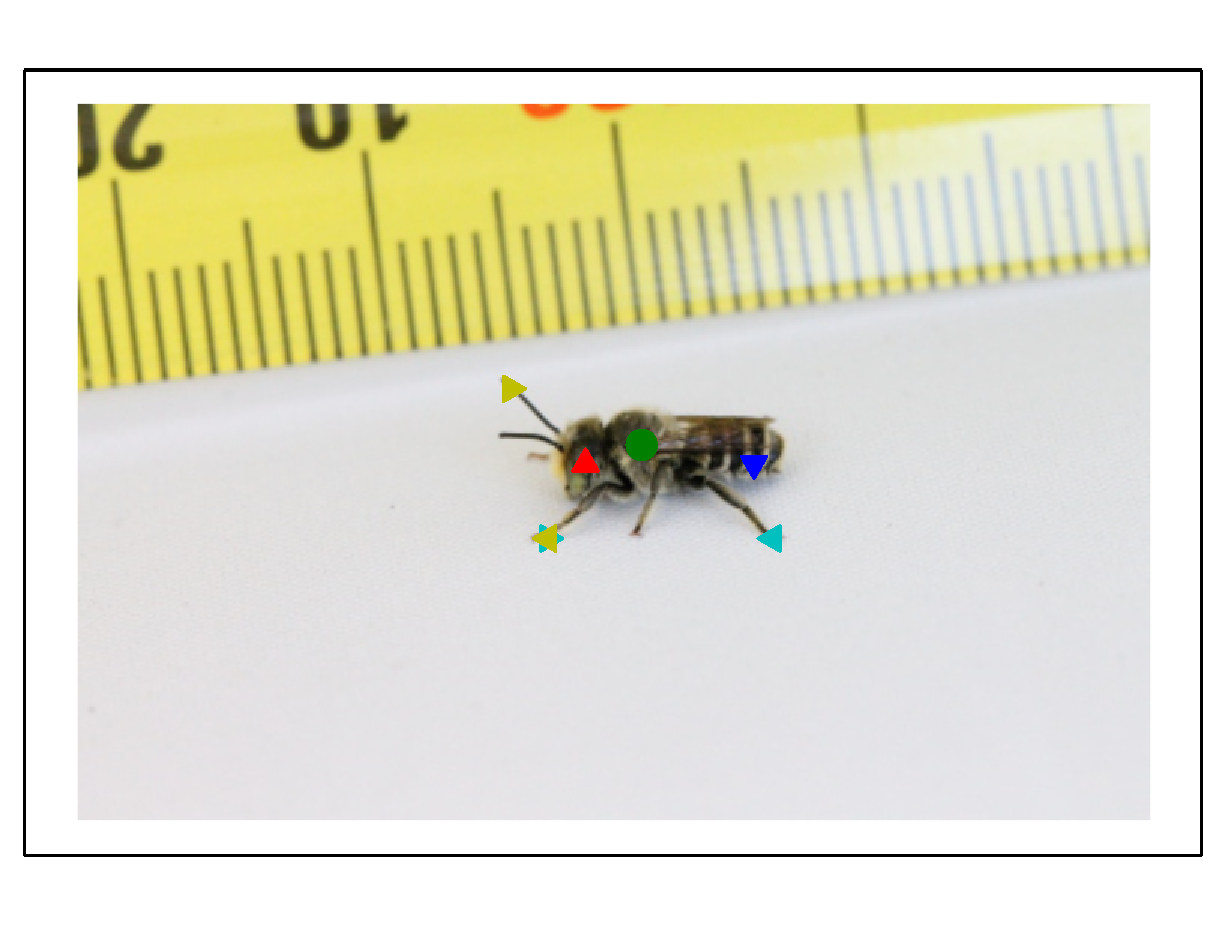
\includegraphics[width=\textwidth]{7p_3.pdf}
                \caption{Seven-part model}
            \end{subfigure}\\
            \begin{subfigure}[b]{0.45\textwidth}
                \centering
                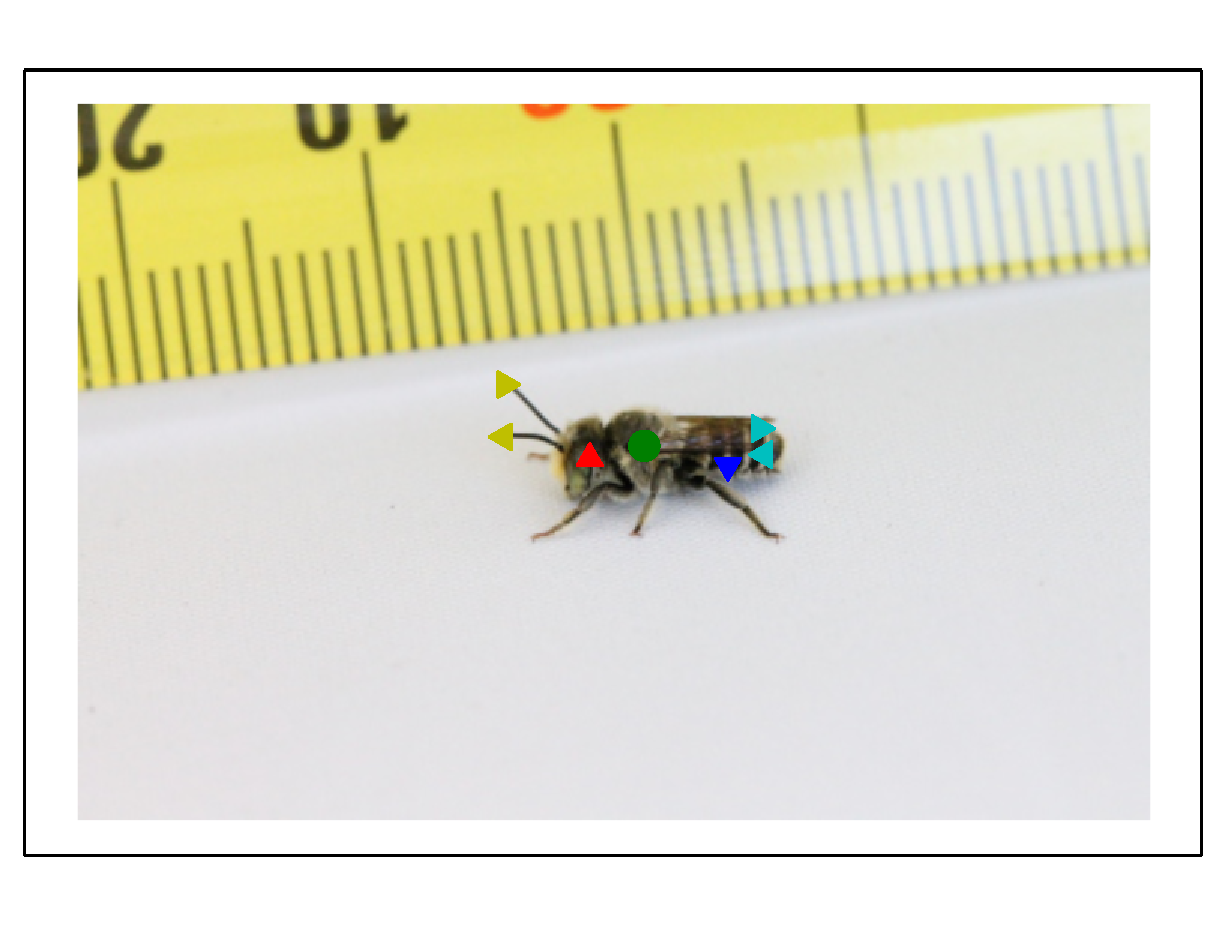
\includegraphics[width=\textwidth]{7pgt_3.pdf}
                \caption{Ground truth}
            \end{subfigure}
            \hspace{0.1\textwidth}\raisebox{15ex}{\framebox[0.25\textwidth]{
                \begin{tabular}{c l}
                {\legends\color{red}{\rotatebox[origin=c]{0}{▲}}}&Head\\
                {\legends\color{green}{●}}&Thorax\\
                {\legends\color{blue}{\rotatebox[origin=c]{180}{▲}}}&Abdomen\\
                {\legends\color{cyan}{\rotatebox[origin=c]{90}{▲}}}&Left Wing\\
                {\legends\color{cyan}{\rotatebox[origin=c]{270}{▲}}}&Right Wing\\
                {\legends\color{yellow}{\rotatebox[origin=c]{90}{▲}}}&Left Antenna\\
                {\legends\color{yellow}{\rotatebox[origin=c]{270}{▲}}}&Right Antenna
                \end{tabular}
            }}\hspace{0.1\textwidth}
            \caption{Predictions on sample test image by number of parts in model}
            \label{fig:37_vis3}
        \end{figure}

    \section{Data augmentation}
        We show the results of augmenting the seven-part model with additional data: images reflected horizontally (axis of reflection is $x=0$), images reflected both horizontally and vertically, and images reflected horizontally and vertically and rotated by 90°.

        It can be seen from figures \ref{fig:aug_pck} and \ref{fig:aug_apk} that data augmentation by reflecting the images horizontally and vertically allows for the most correct and accurate model. It is curious that augmenting the data by said reflections along with rotations by 90° results in less accurate predictions. One may hypothesize that the increased variety of bee poses that rotation by 90° creates adds noise to the parameters learned by the graphical model and therefore reduces its utility.

        \begin{figure}
            \centering
                    \begin{tikzpicture}
                        \begin{axis}[width=0.7\textwidth,
                            ylabel=Probability of Correct Keypoint (\%),
                            symbolic x coords={no aug, h ref,h+v ref,h+v ref+rot}, xtick=data,
                        legend style={at={(1.1,0.5)}, anchor=west}]
                        \addplot[only marks,color=red,mark=triangle*] coordinates {
                            (no aug, 63)
                            (h ref, 72)
                            (h+v ref, 78)
                            (h+v ref+rot, 74)
                        };
                        \addplot[only marks,color=green,mark=*] coordinates {
                            (no aug, 64)
                            (h ref, 65)
                            (h+v ref, 72)
                            (h+v ref+rot, 71)
                        };
                        \addplot[only marks,color=blue,mark=triangle*, mark options={rotate=180}] coordinates {
                            (no aug, 56)
                            (h ref, 56)
                            (h+v ref, 63)
                            (h+v ref+rot, 61)
                        };
                        \addplot[only marks,color=cyan,mark=triangle*, mark options={rotate=90}] coordinates {
                            (no aug, 28)
                            (h ref, 26)
                            (h+v ref, 24)
                            (h+v ref+rot, 19)
                        };
                        \addplot[only marks,color=cyan,mark=triangle*, mark options={rotate=270}] coordinates {
                            (no aug, 22)
                            (h ref, 24)
                            (h+v ref, 25)
                            (h+v ref+rot, 33)
                        };
                        \addplot[only marks,color=yellow,mark=halfsquare left*] coordinates {
                            (no aug, 28)
                            (h ref, 35)
                            (h+v ref, 32)
                            (h+v ref+rot, 30)
                        };
                        \addplot[only marks,color=yellow,mark=halfsquare right*] coordinates {
                            (no aug, 25)
                            (h ref, 33)
                            (h+v ref, 33)
                            (h+v ref+rot, 41)
                        };
                        \addplot[only marks,color=black,mark=square*] coordinates {
                            (no aug, 61)
                            (h ref, 64.3)
                            (h+v ref, 71)
                            (h+v ref+rot, 68.7)
                        };
                        \addplot[only marks,color=black,mark=square, mark options={rotate=180}] coordinates {
                            (no aug, 40.9)
                            (h ref, 44.4)
                            (h+v ref, 46.7)
                            (h+v ref+rot, 47)
                        };
                        \legend{Head, Thorax, Abdomen, L Wing, R Wing, L Antenna, R Antenna, Mean (3p), Mean (7p)}
                        \end{axis}
                    \end{tikzpicture}
                \caption{PCK by parts in model for HOG cell size 4}
                \label{fig:aug_pck}
            \end{figure}
            \begin{figure}
                \centering
                \begin{tikzpicture}
                    \begin{axis}[width=0.7\textwidth,
                        ylabel=Average Precision of Keypoints (\%),
                        symbolic x coords={no aug, h ref,h+v ref,h+v ref+rot}, xtick=data,
                        legend style={at={(1.1,0.5)}, anchor=west}]
                    \addplot[only marks,color=red,mark=triangle*] coordinates {
                            (no aug, 66.5)
                            (h ref, 73.1)
                            (h+v ref, 72.7)
                            (h+v ref+rot, 73.9)
                        };
                        \addplot[only marks,color=green,mark=*] coordinates {
                            (no aug, 62.2)
                            (h ref, 70.1)
                            (h+v ref, 74.5)
                            (h+v ref+rot, 68.3)
                        };
                        \addplot[only marks,color=blue,mark=triangle*, mark options={rotate=180}] coordinates {
                            (no aug, 51.2)
                            (h ref, 57)
                            (h+v ref, 57.1)
                            (h+v ref+rot, 56.2)
                        };
                        \addplot[only marks,color=cyan,mark=triangle*, mark options={rotate=90}] coordinates {
                            (no aug, 11)
                            (h ref, 8)
                            (h+v ref, 8)
                            (h+v ref+rot, 5.3)
                        };
                        \addplot[only marks,color=cyan,mark=triangle*, mark options={rotate=270}] coordinates {
                            (no aug, 9)
                            (h ref, 9.5)
                            (h+v ref, 13.1)
                            (h+v ref+rot, 15.3)
                        };
                        \addplot[only marks,color=yellow,mark=halfsquare left*] coordinates {
                            (no aug, 17)
                            (h ref, 26.1)
                            (h+v ref, 21.8)
                            (h+v ref+rot, 14.1)
                        };
                        \addplot[only marks,color=yellow,mark=halfsquare right*] coordinates {
                            (no aug, 18.4)
                            (h ref, 22)
                            (h+v ref, 22.7)
                            (h+v ref+rot, 30.2)
                        };
                        \addplot[only marks,color=black,mark=square*] coordinates {
                            (no aug, 60)
                            (h ref, 66.7)
                            (h+v ref, 68.1)
                            (h+v ref+rot, 66.1)
                        };
                        \addplot[only marks,color=black,mark=square, mark options={rotate=180}] coordinates {
                            (no aug, 40.9)
                            (h ref, 38)
                            (h+v ref, 38.6)
                            (h+v ref+rot, 37.6)
                        };
                        \legend{Head, Thorax, Abdomen, L Wing, R Wing, L Antenna, R Antenna, Mean (3p), Mean (7p)}
                    \end{axis}
                \end{tikzpicture}
                \caption{APK by parts in model for HOG cell size 4}
                \label{fig:aug_apk}
        \end{figure}

        \begin{figure}[p]
            \centering
            \begin{subfigure}[b]{0.45\textwidth}
                \centering
                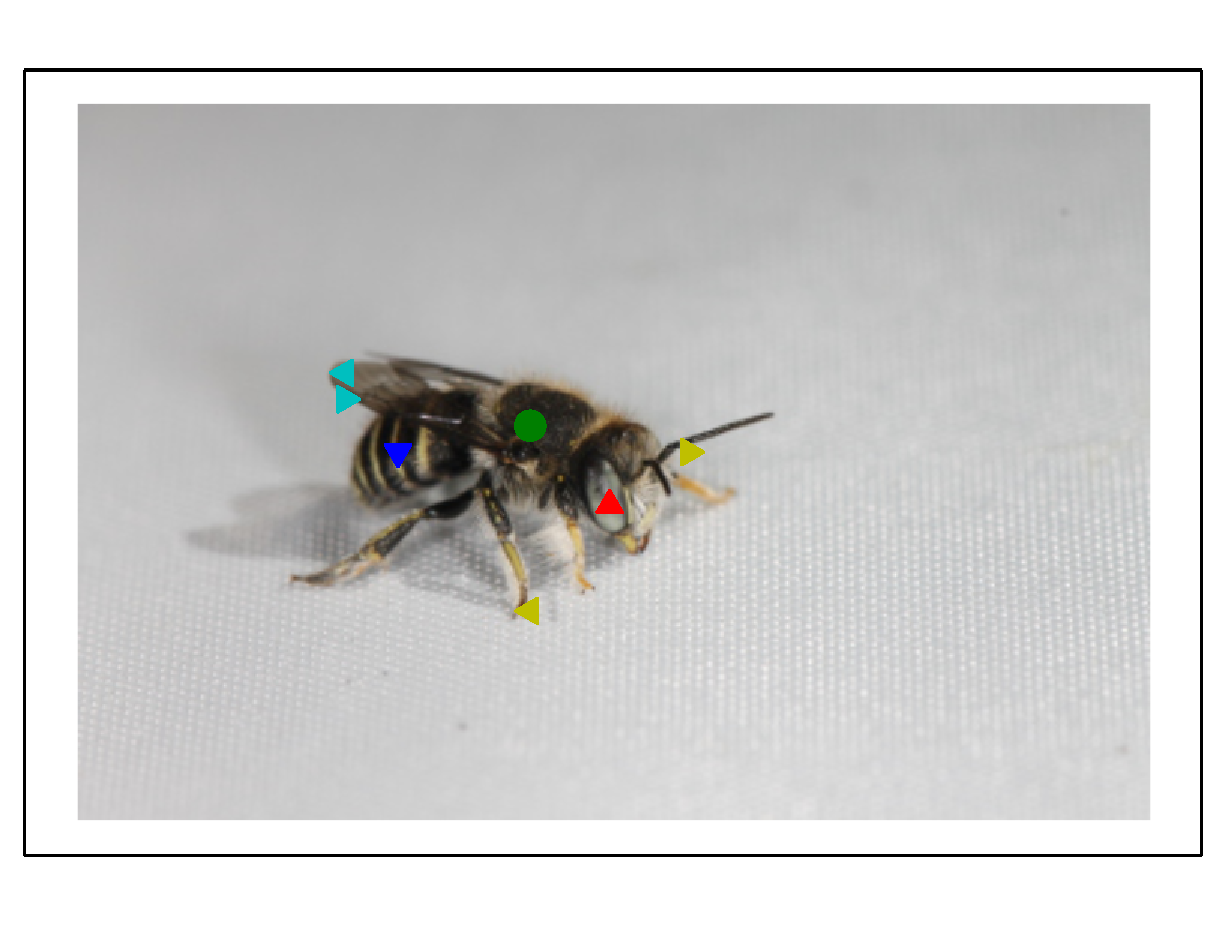
\includegraphics[width=\textwidth]{7p_1.pdf}
                \caption{No augmentation}
            \end{subfigure}
            \begin{subfigure}[b]{0.45\textwidth}
                \centering
                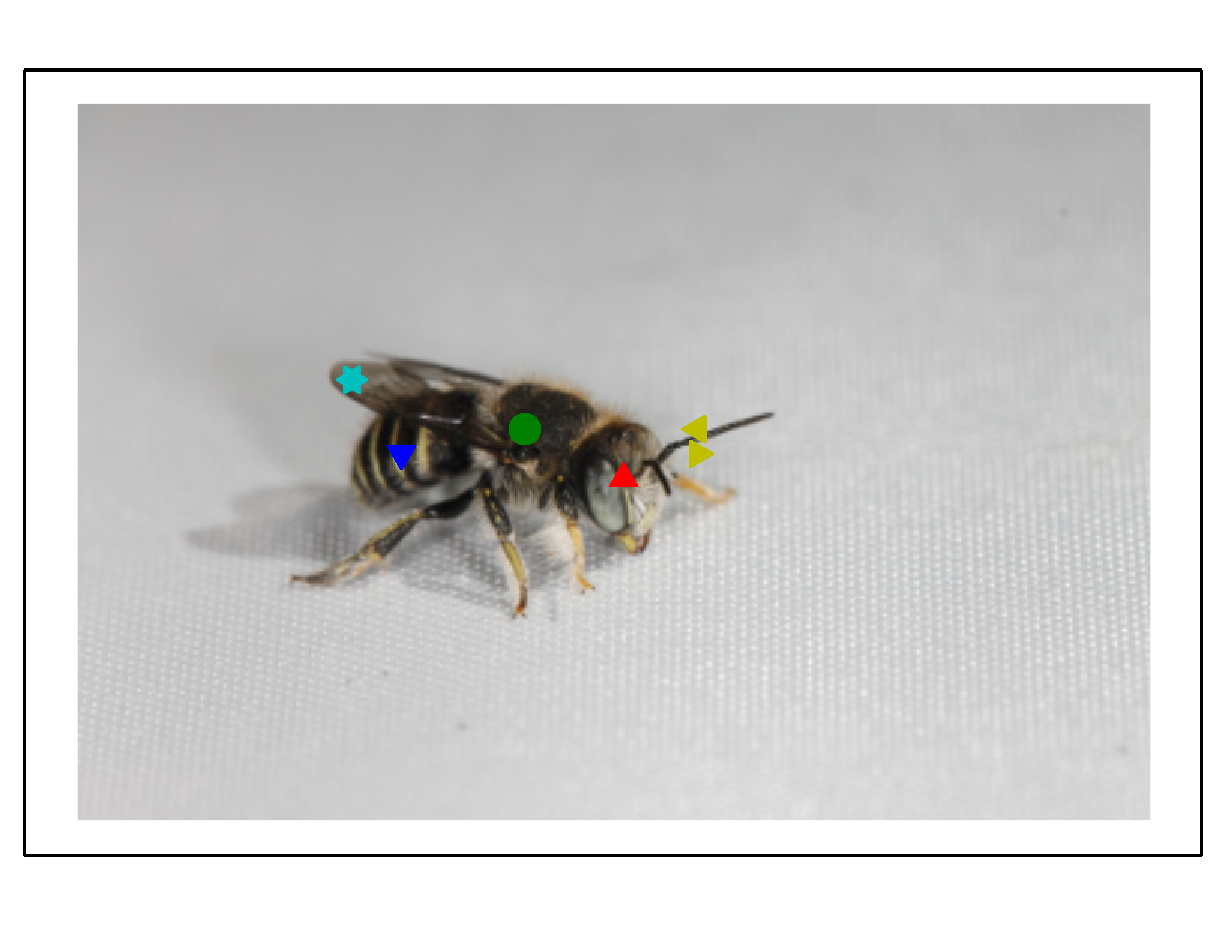
\includegraphics[width=\textwidth]{refl_1.pdf}
                \caption{Reflections along the $y$-axis}
            \end{subfigure}
            \begin{subfigure}[b]{0.45\textwidth}
                \centering
                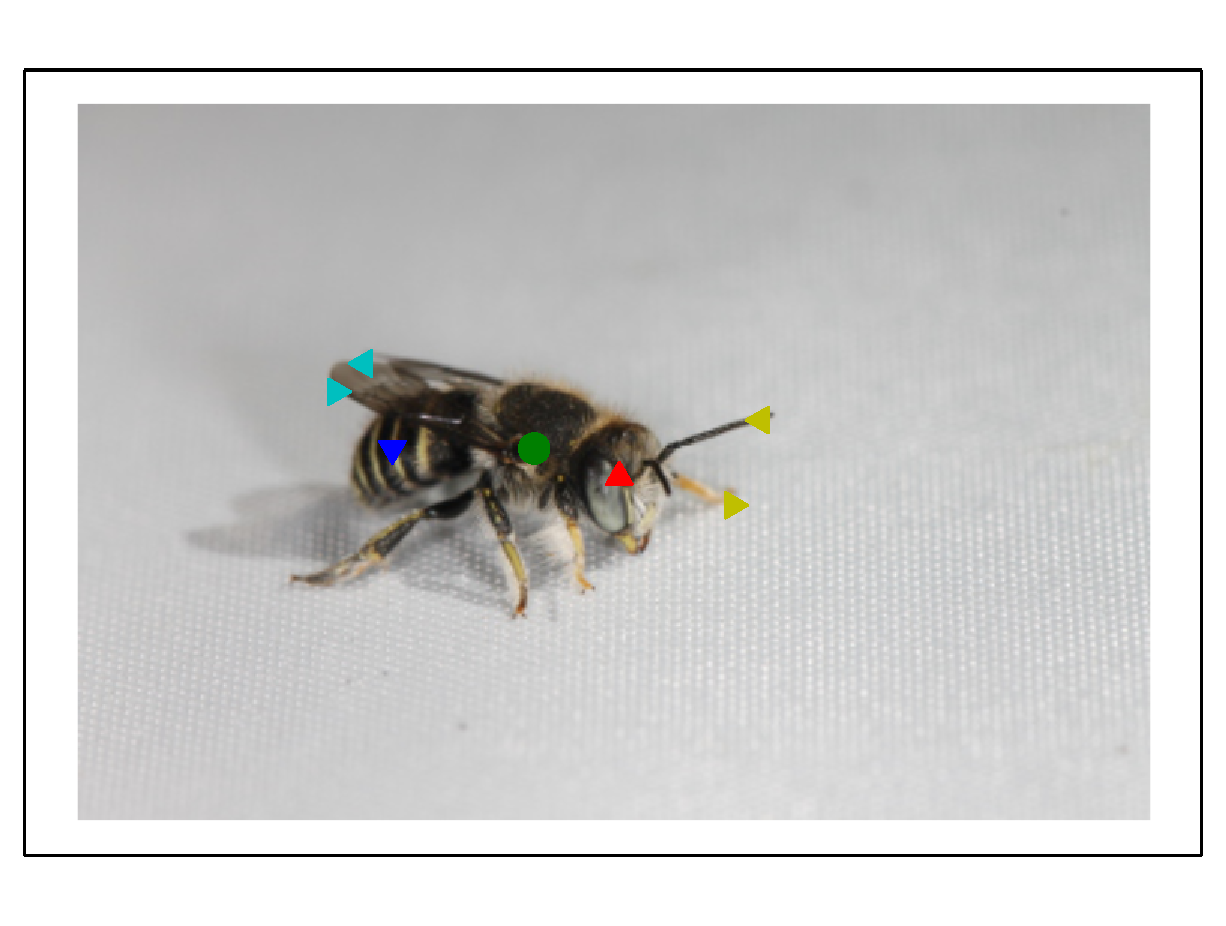
\includegraphics[width=\textwidth]{2refl_1.pdf}
                \caption{Reflections along the $x$- and $y$-axes\\\hspace{0pt}}
            \end{subfigure}
            \begin{subfigure}[b]{0.45\textwidth}
                \centering
                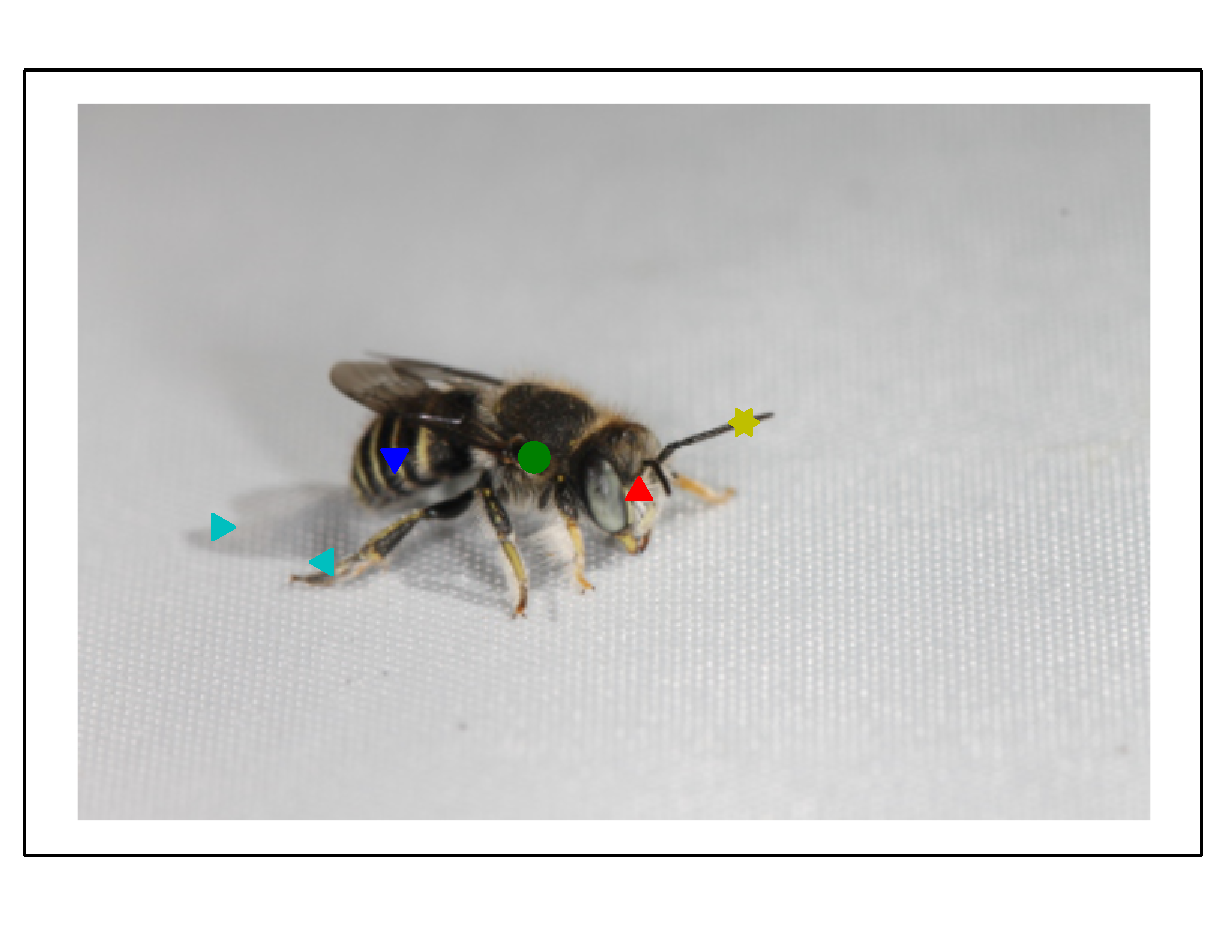
\includegraphics[width=\textwidth]{2reflrot_1.pdf}
                \caption{Reflections along the $x$- and $y$-axes and rotations by 90°}
            \end{subfigure}
            \begin{subfigure}[b]{0.45\textwidth}
                \centering
                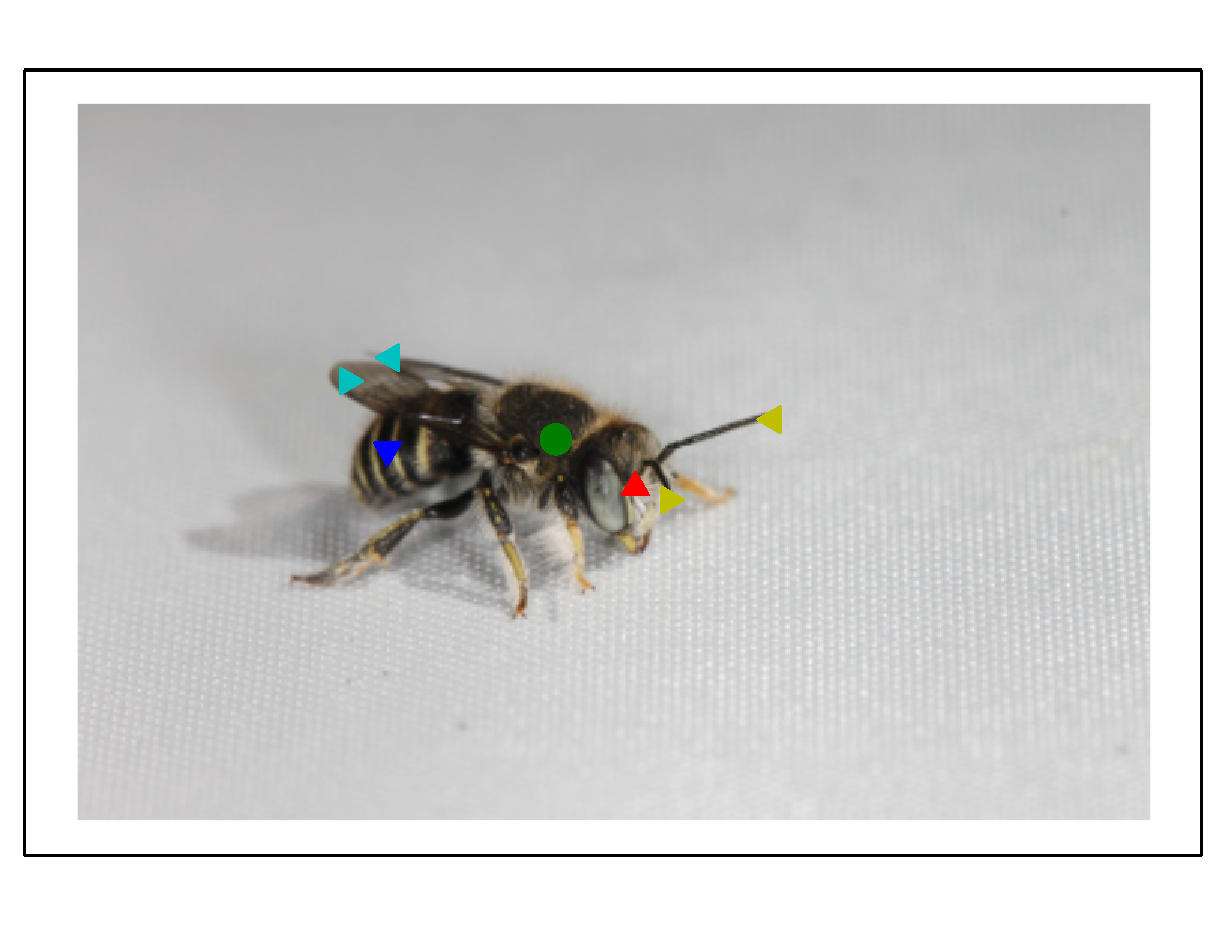
\includegraphics[width=\textwidth]{7pgt_1.pdf}
                \caption{Ground truth}
            \end{subfigure}
            \hspace{0.1\textwidth}\raisebox{15ex}{\framebox[0.25\textwidth]{
                \begin{tabular}{c l}
                {\legends\color{red}{\rotatebox[origin=c]{0}{▲}}}&Head\\
                {\legends\color{green}{●}}&Thorax\\
                {\legends\color{blue}{\rotatebox[origin=c]{180}{▲}}}&Abdomen\\
                {\legends\color{cyan}{\rotatebox[origin=c]{90}{▲}}}&Left Wing\\
                {\legends\color{cyan}{\rotatebox[origin=c]{270}{▲}}}&Right Wing\\
                {\legends\color{yellow}{\rotatebox[origin=c]{90}{▲}}}&Left Antenna\\
                {\legends\color{yellow}{\rotatebox[origin=c]{270}{▲}}}&Right Antenna
                \end{tabular}
            }}\hspace{0.1\textwidth}
            \caption{Predictions on sample test image by the type of data augmentation}
            \label{fig:aug_vis1}
        \end{figure} 
        \begin{figure}[p]
            \centering
            \begin{subfigure}[b]{0.45\textwidth}
                \centering
                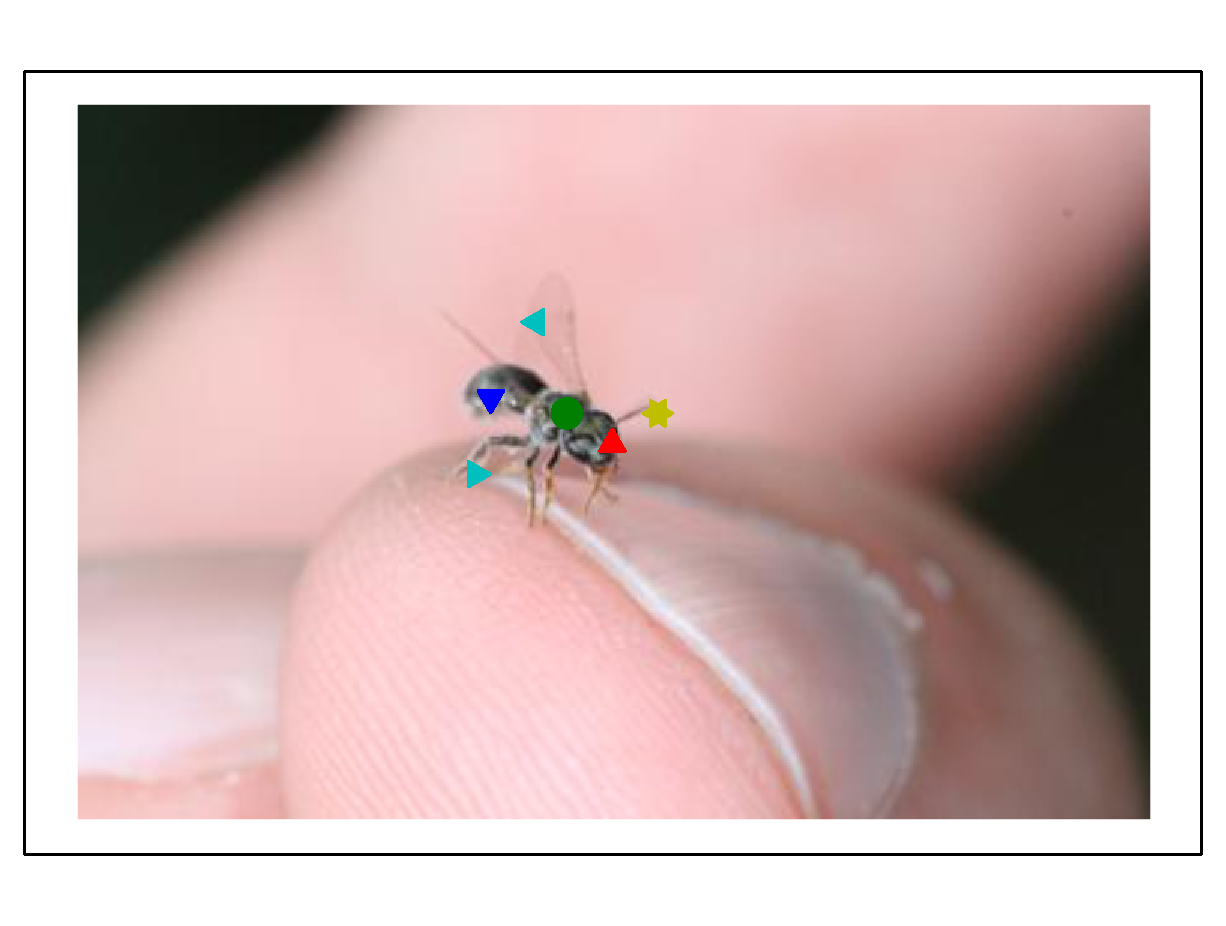
\includegraphics[width=\textwidth]{7p_2.pdf}
                \caption{No augmentation}
            \end{subfigure}
            \begin{subfigure}[b]{0.45\textwidth}
                \centering
                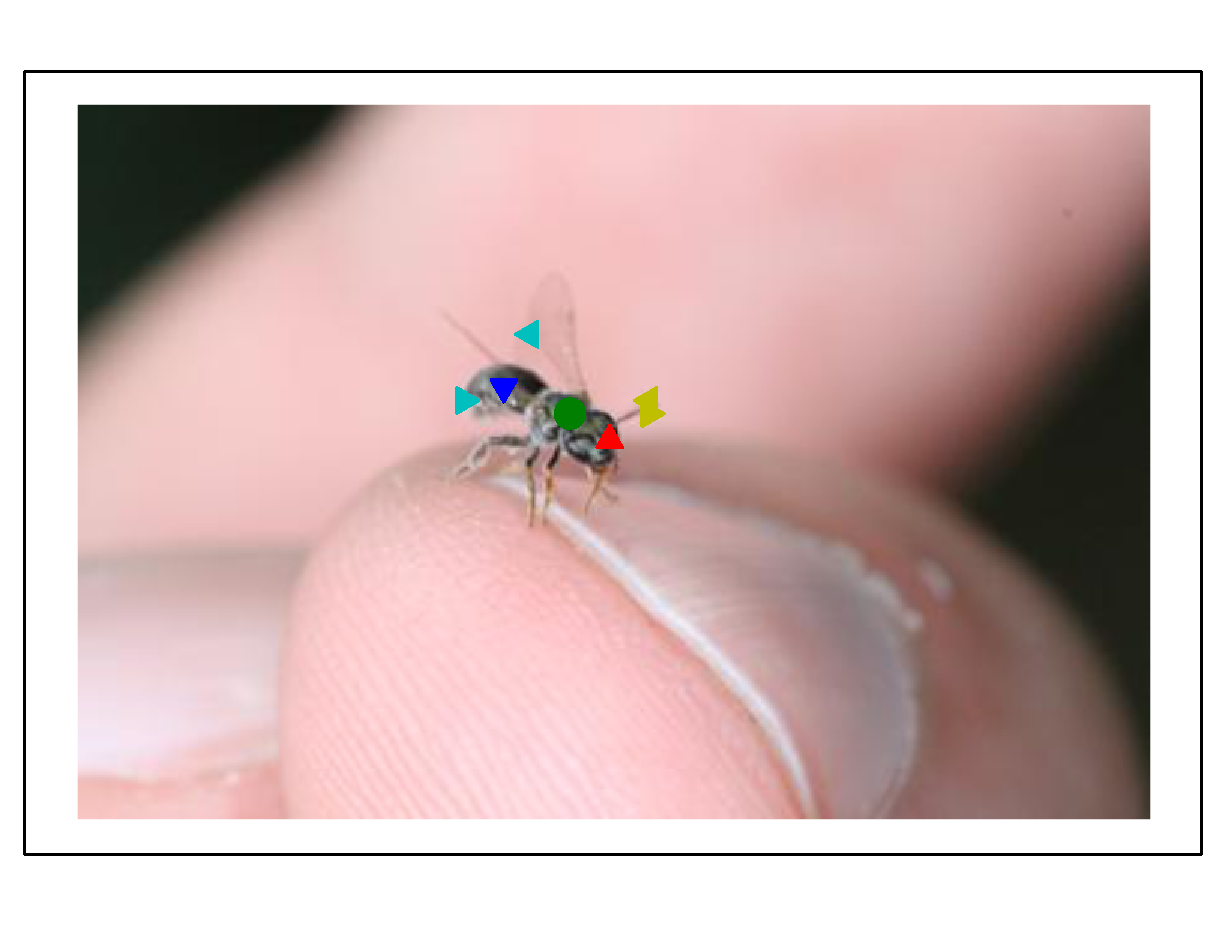
\includegraphics[width=\textwidth]{refl_2.pdf}
                \caption{Reflections along the $y$-axis}
            \end{subfigure}
            \begin{subfigure}[b]{0.45\textwidth}
                \centering
                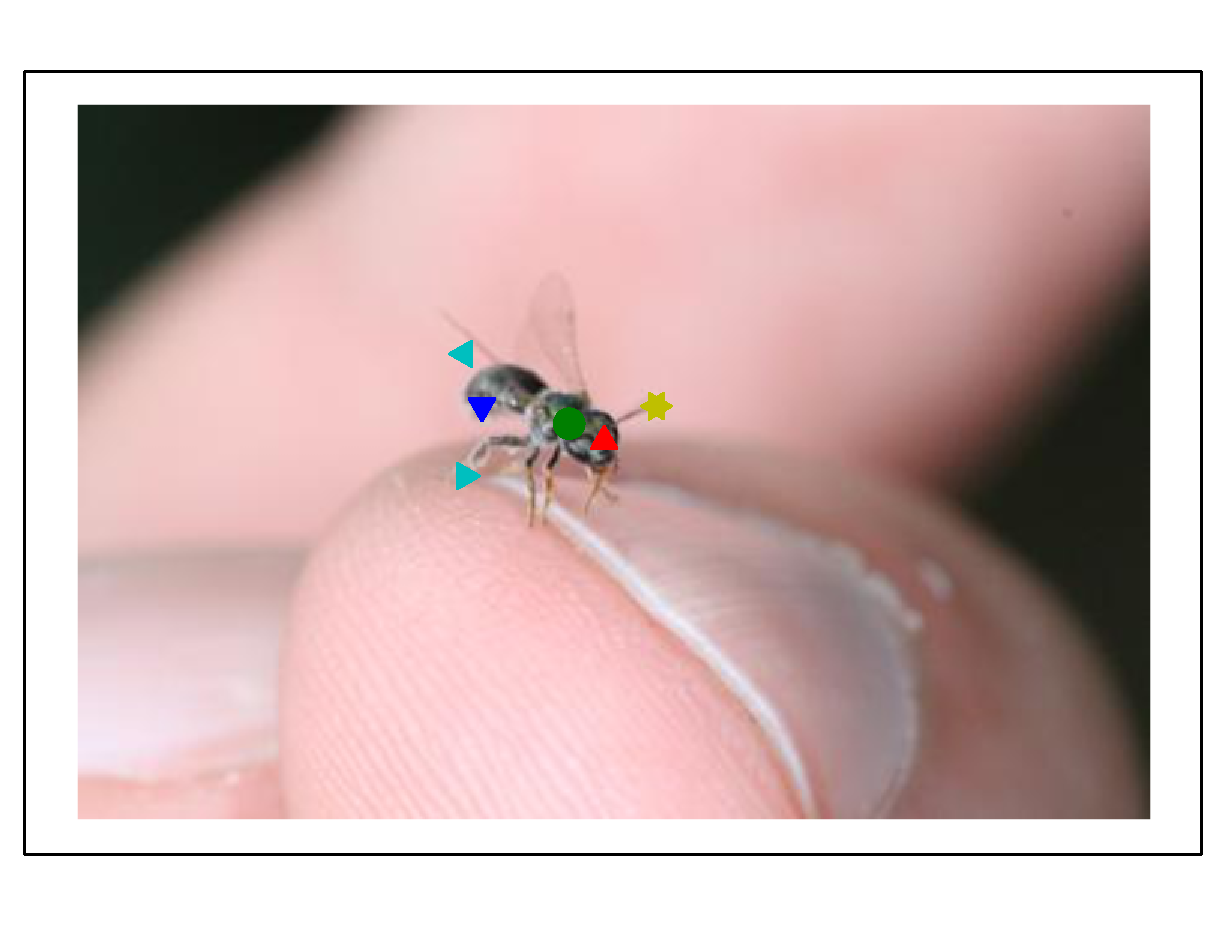
\includegraphics[width=\textwidth]{2refl_2.pdf}
                \caption{Reflections along the $x$- and $y$-axes\\\hspace{0pt}}
            \end{subfigure}
            \begin{subfigure}[b]{0.45\textwidth}
                \centering
                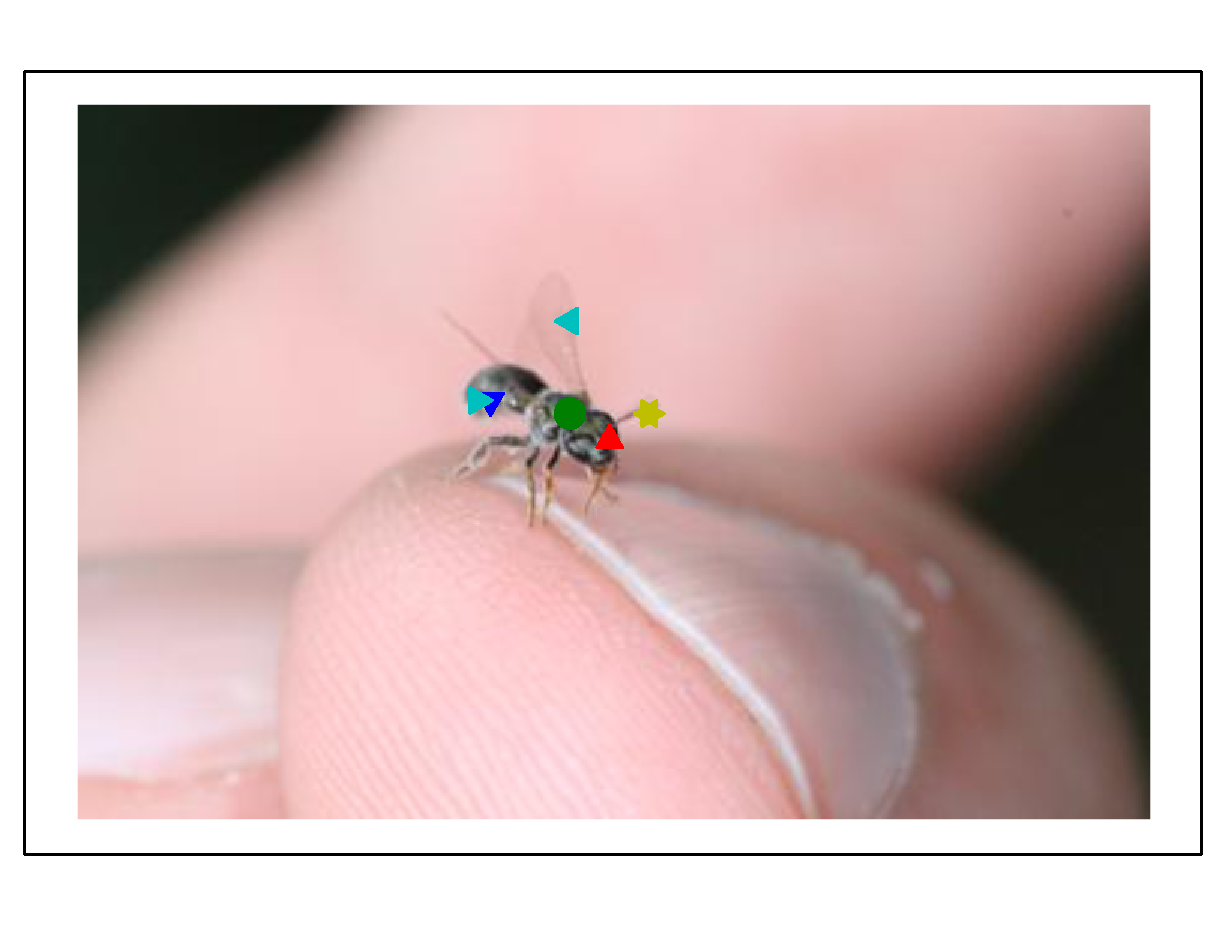
\includegraphics[width=\textwidth]{2reflrot_2.pdf}
                \caption{Reflections along the $x$- and $y$-axes and rotations by 90°}
            \end{subfigure}
            \begin{subfigure}[b]{0.45\textwidth}
                \centering
                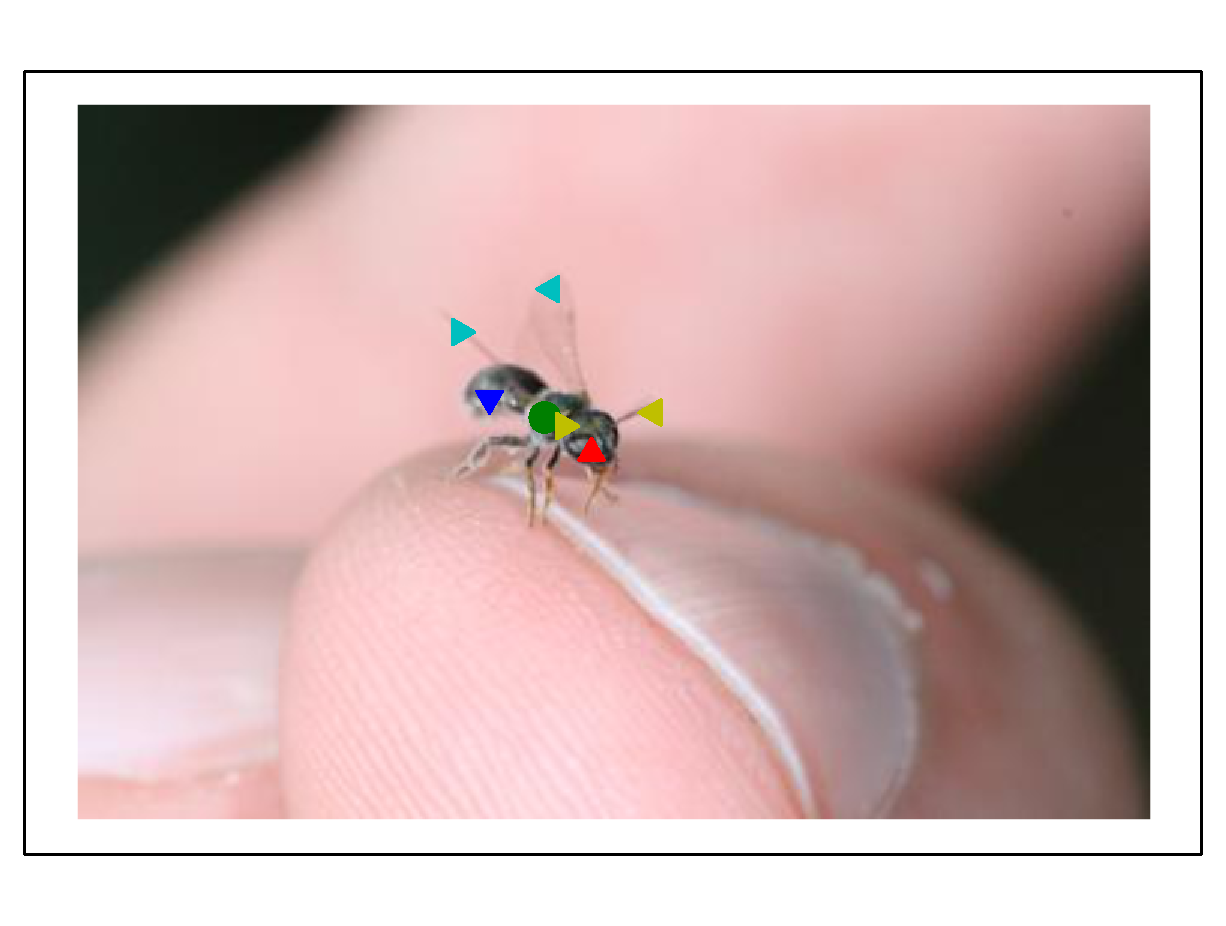
\includegraphics[width=\textwidth]{7pgt_2.pdf}
                \caption{Ground truth}
            \end{subfigure}
            \hspace{0.1\textwidth}\raisebox{15ex}{\framebox[0.25\textwidth]{
                \begin{tabular}{c l}
                {\legends\color{red}{\rotatebox[origin=c]{0}{▲}}}&Head\\
                {\legends\color{green}{●}}&Thorax\\
                {\legends\color{blue}{\rotatebox[origin=c]{180}{▲}}}&Abdomen\\
                {\legends\color{cyan}{\rotatebox[origin=c]{90}{▲}}}&Left Wing\\
                {\legends\color{cyan}{\rotatebox[origin=c]{270}{▲}}}&Right Wing\\
                {\legends\color{yellow}{\rotatebox[origin=c]{90}{▲}}}&Left Antenna\\
                {\legends\color{yellow}{\rotatebox[origin=c]{270}{▲}}}&Right Antenna
                \end{tabular}
            }}\hspace{0.1\textwidth}
            \caption{Predictions on sample test image by the type of data augmentation}
            \label{fig:aug_vis2}
        \end{figure} 
        \begin{figure}[p]
            \centering
            \begin{subfigure}[b]{0.45\textwidth}
                \centering
                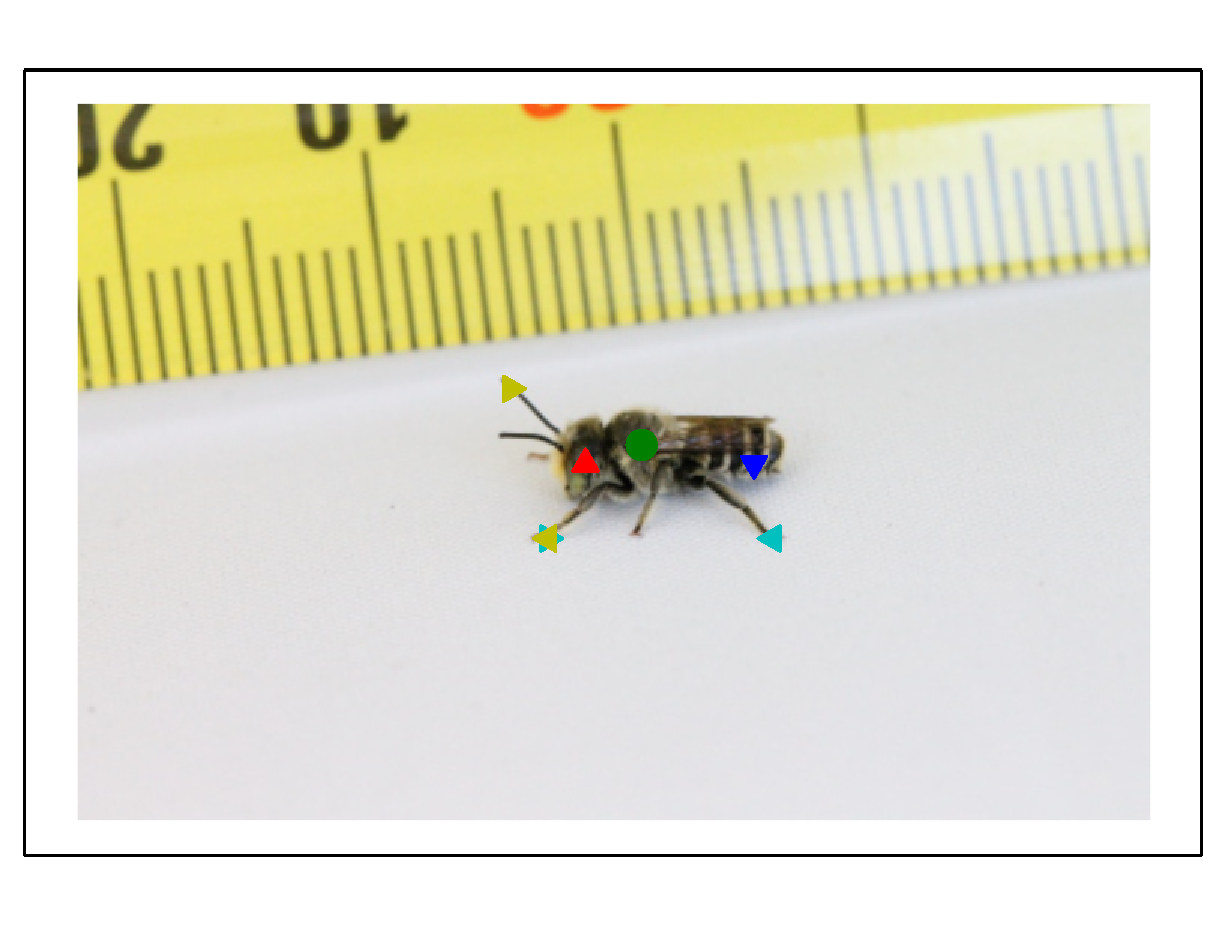
\includegraphics[width=\textwidth]{7p_3.pdf}
                \caption{No augmentation}
            \end{subfigure}
            \begin{subfigure}[b]{0.45\textwidth}
                \centering
                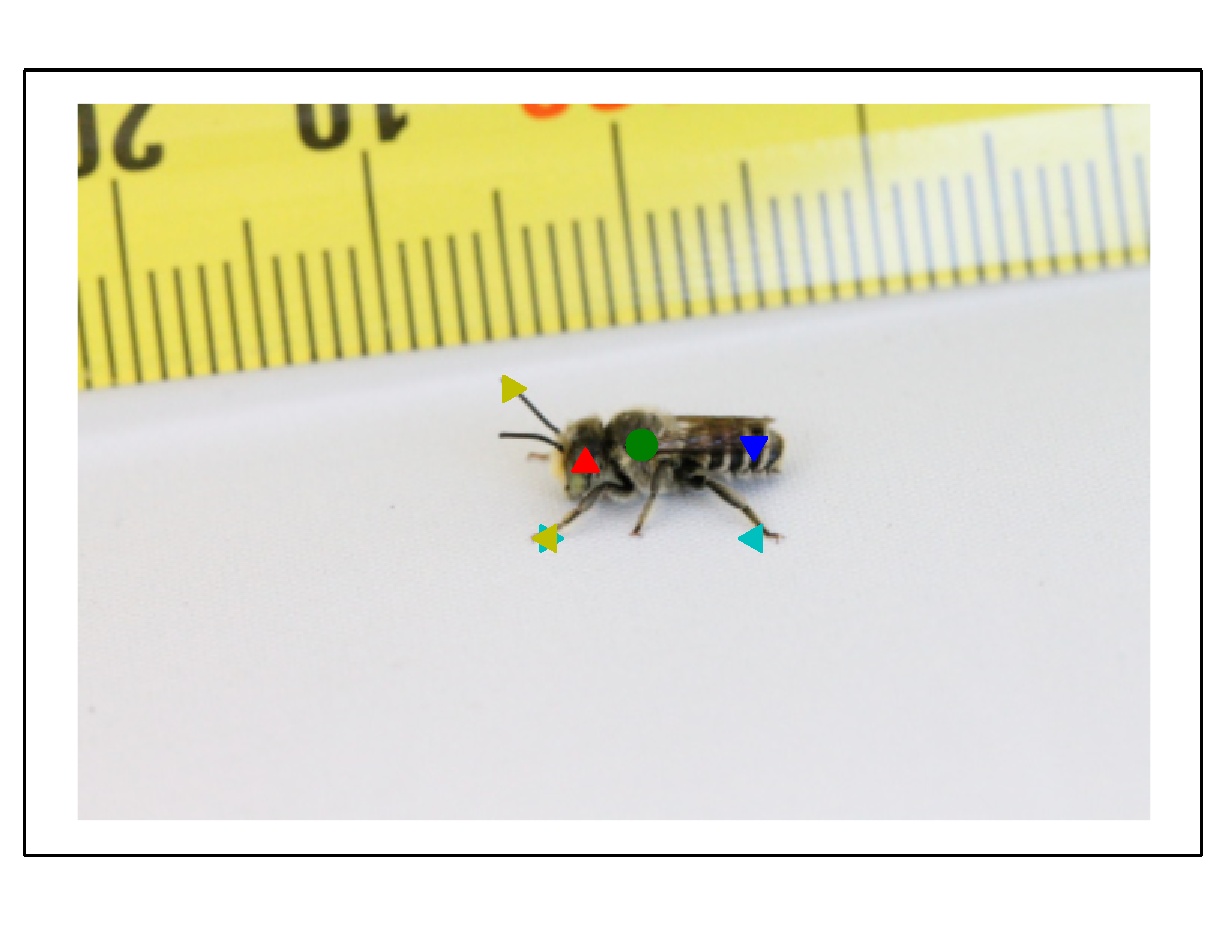
\includegraphics[width=\textwidth]{refl_3.pdf}
                \caption{Reflections along the $y$-axis}
            \end{subfigure}
            \begin{subfigure}[b]{0.45\textwidth}
                \centering
                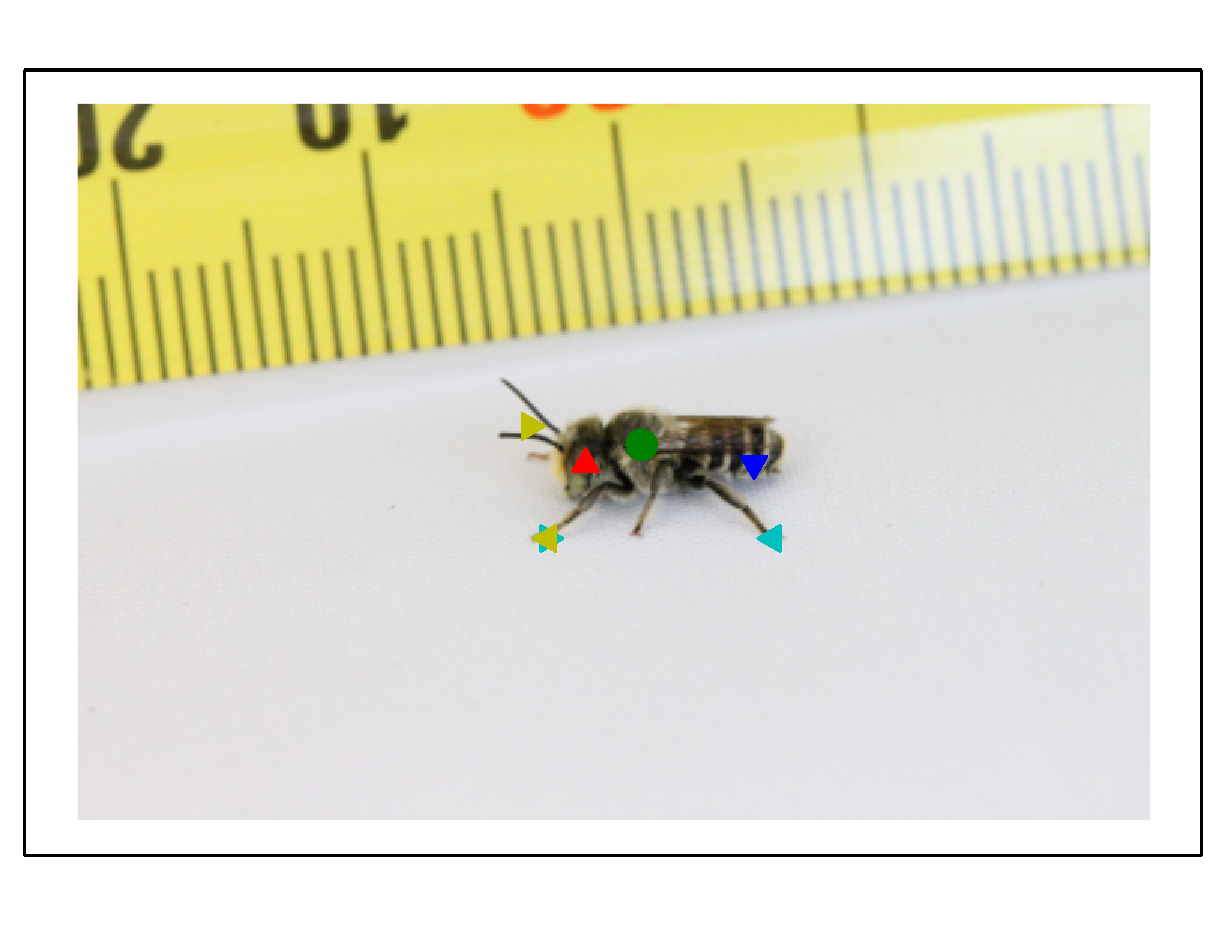
\includegraphics[width=\textwidth]{2refl_3.pdf}
                \caption{Reflections along the $x$- and $y$-axes\\\hspace{0pt}}
            \end{subfigure}
            \begin{subfigure}[b]{0.45\textwidth}
                \centering
                \includegraphics[width=\textwidth]{2reflrot_3.pdf}
                \caption{Reflections along the $x$- and $y$-axes and rotations by 90°}
            \end{subfigure}
            \begin{subfigure}[b]{0.45\textwidth}
                \centering
                \includegraphics[width=\textwidth]{7pgt_3.pdf}
                \caption{Ground truth}
            \end{subfigure}
            \hspace{0.1\textwidth}\raisebox{15ex}{\framebox[0.25\textwidth]{
                \begin{tabular}{c l}
                {\legends\color{red}{\rotatebox[origin=c]{0}{▲}}}&Head\\
                {\legends\color{green}{●}}&Thorax\\
                {\legends\color{blue}{\rotatebox[origin=c]{180}{▲}}}&Abdomen\\
                {\legends\color{cyan}{\rotatebox[origin=c]{90}{▲}}}&Left Wing\\
                {\legends\color{cyan}{\rotatebox[origin=c]{270}{▲}}}&Right Wing\\
                {\legends\color{yellow}{\rotatebox[origin=c]{90}{▲}}}&Left Antenna\\
                {\legends\color{yellow}{\rotatebox[origin=c]{270}{▲}}}&Right Antenna
                \end{tabular}
            }}\hspace{0.1\textwidth}
            \caption{Predictions on sample test image by the type of data augmentation}
            \label{fig:aug_vis3}
        \end{figure}

    \section{Summary}
        Is is clearly seen that the model that results in the best predictions is one that uses the 7-part graphical model, $4\times4$ HOG cells and data augmentation by reflection along the horizontal and vertical axes. That model is characterised by an average (3-part) PCK of 71\% and average (3-part) APK of 68.1\%.

\chapter{Reflection}
    \section{Future direction}
        The model described is has an average of 71\% success rate of correct three-part pose estimations on the test set. It is possible that by using a pose estimation model developed for use on bees, as opposed to on humans, this success rate can be improved. Such a model could, for example, account for the increased variance in bee poses and the differing proportions and appearances between species.

        This bee pose estimation algorithm may find use in bee classification, by allowing the feature extractor to locate the bee, and the relevant bee parts, in the image. Further, this could lead to a crowdsourced bee population data gathering tool, as described in chapter 1.

    \section{Acknowledgements}
        I would like to thank Dr Cheng Soon Ong and Dr Stephen Gould for supervising this project. I would also like to thank Dr Anoop Cherian for his assistance.

\chapter{References}

Agriculture and Consumer Protection Department of the Food and Agriculture Organization of the United Nations, 2005.

Chen X. and Yuille A., 2014. \textit{Articulated Pose Estimation by a Graphical Model with Image Dependent Pairwise Relations}. NIPS 2014.
\url{http://www.stat.ucla.edu/~xianjie.chen/projects/pose_estimation/pose_estimation.html}

Everingham M. et al., 2010. `The pascal visual object classes (voc) challenge'. \textit{International Journal of Computer Vision}, vol. 88, no. 2.

Santana et al. 2014. `A reference process for automating bee species identification based on wing images and digital image processing'. \textit{Ecological Informatics}, no. 0, vol. 24.

Yang Y. and Ramanan D., 2011. \textit{Articulated Pose Estimation using Flexible Mixtures of Parts}. CVPR 2011.

Yang Y. and Ramanan D., 2013. `Articulated Human Detection with Flexible Mixtures of Parts'. \textit{IEEE Transactions on Pattern Analysis and Machine Intelligence}.



\appendix
\chapter{The BEES Dataset}
    The BEES dataset was developed for this project. It is composed of 640 photographs displaying bees of various species in diverse positions.

    Each photograph in the BEES dataset displays one bee. The bee is labelled with the coordinates in the image of the middle of its head, thorax, and abdomen, as well as the tip of its right wing, left wing, right antenna and left antenna. However, in the case that one of these bee parts is occluded, no position is listed for that part. Difficult images are also tagged, and the bee is labelled with its species. Examples shown in figure \ref{fig:BEES_examples}.

\begin{figure}[h]
    \centering
    \includegraphics[width=0.424\textwidth]{b1.pdf}\hfill
    \includegraphics[width=0.424\textwidth]{b2.pdf}
    \includegraphics[width=0.424\textwidth]{b3.pdf}\hfill
    \includegraphics[width=0.424\textwidth]{b4.pdf}
    \caption{Examples of annotated images in the BEES dataset}
    \label{fig:BEES_examples}
\end{figure}

\chapter{Labelling tool}
    In the process of developing the BEES dataset, a GUI labelling tool was written. The tool guides the user through the process of labelling all images in the set. Upon reading a list of file names, images appear on the screen one by one and the user is asked to click on bee parts in order to mark them. The user may also declare the part occluded, as well as mark the entire image as difficult. Progress may be saved to and restored from file. The end output is a JSON file specifying image file names, image sizes, part positions or lack thereof, and difficult image flags. A screenshot of the tool is shown in figure \ref{fig:Labelling_screenshot}.

    \begin{figure}[h]
        \centering
        \includegraphics[width=\textwidth]{features_tool.png}\hfill
        \caption{The labelling tool}
        \label{fig:Labelling_screenshot}
    \end{figure}

\chapter{Python scripts}
    \section{Visualisation tool}
        \begin{figure}[h]
            \centering
            \includegraphics[width=\textwidth]{visualisation_tool.png}\hfill
            \caption{The visualisation tool}
            \label{fig:Visualisation_screenshot}
        \end{figure}
        A visualisation tool was developed to aid in debugging code, observing performance, and developing visualisations for publication. It is able to visualise predictions, labels that are input into the Matlab code, as well labels in a JSON file. The images are read and overlaid with marked parts. A legend is provided. A screenshot is shown in figure \ref{fig:Visualisation_screenshot}.

    \section{Dataset randomisation and preparation tool}
        A tool was developed that prepares the BEES dataset for input into the Matlab program. It reads a JSON file containing image file names and feature labels; shuffles the images; filters the images such that only ones with complete annotations (no parts occluded or missing) remain; and divides the images into six sets of 50. The images are then copied into appropriate folders in the previously determined random order, and the labels are saved in a .mat file for Matlab to read, as well as in a JSON file to maintain the ability to easily read them with Python.
    
    \section{Results reading tool}
        A Python class was developed that provides an interface for reading the results of Matlab predictions. It reads the Matlab files output by the prediction code and converts them into Python objects. It is used in the Visualisation Tool, but also available for import as a standalone module.

\end{document}
